\chapter{PCB 2.0 改进设计和测试}
\label{cha:PCB-v2}

本章设计源文件和历史版本详见\url{https://github.com/TingliangZhang/Misaka-PCB-v2},其中包括分层原理图、PCB设计、Gerber。

总原理图如图~\ref{fig:Circuit-1}所示。

\begin{figure}[htbp]
    \centering
    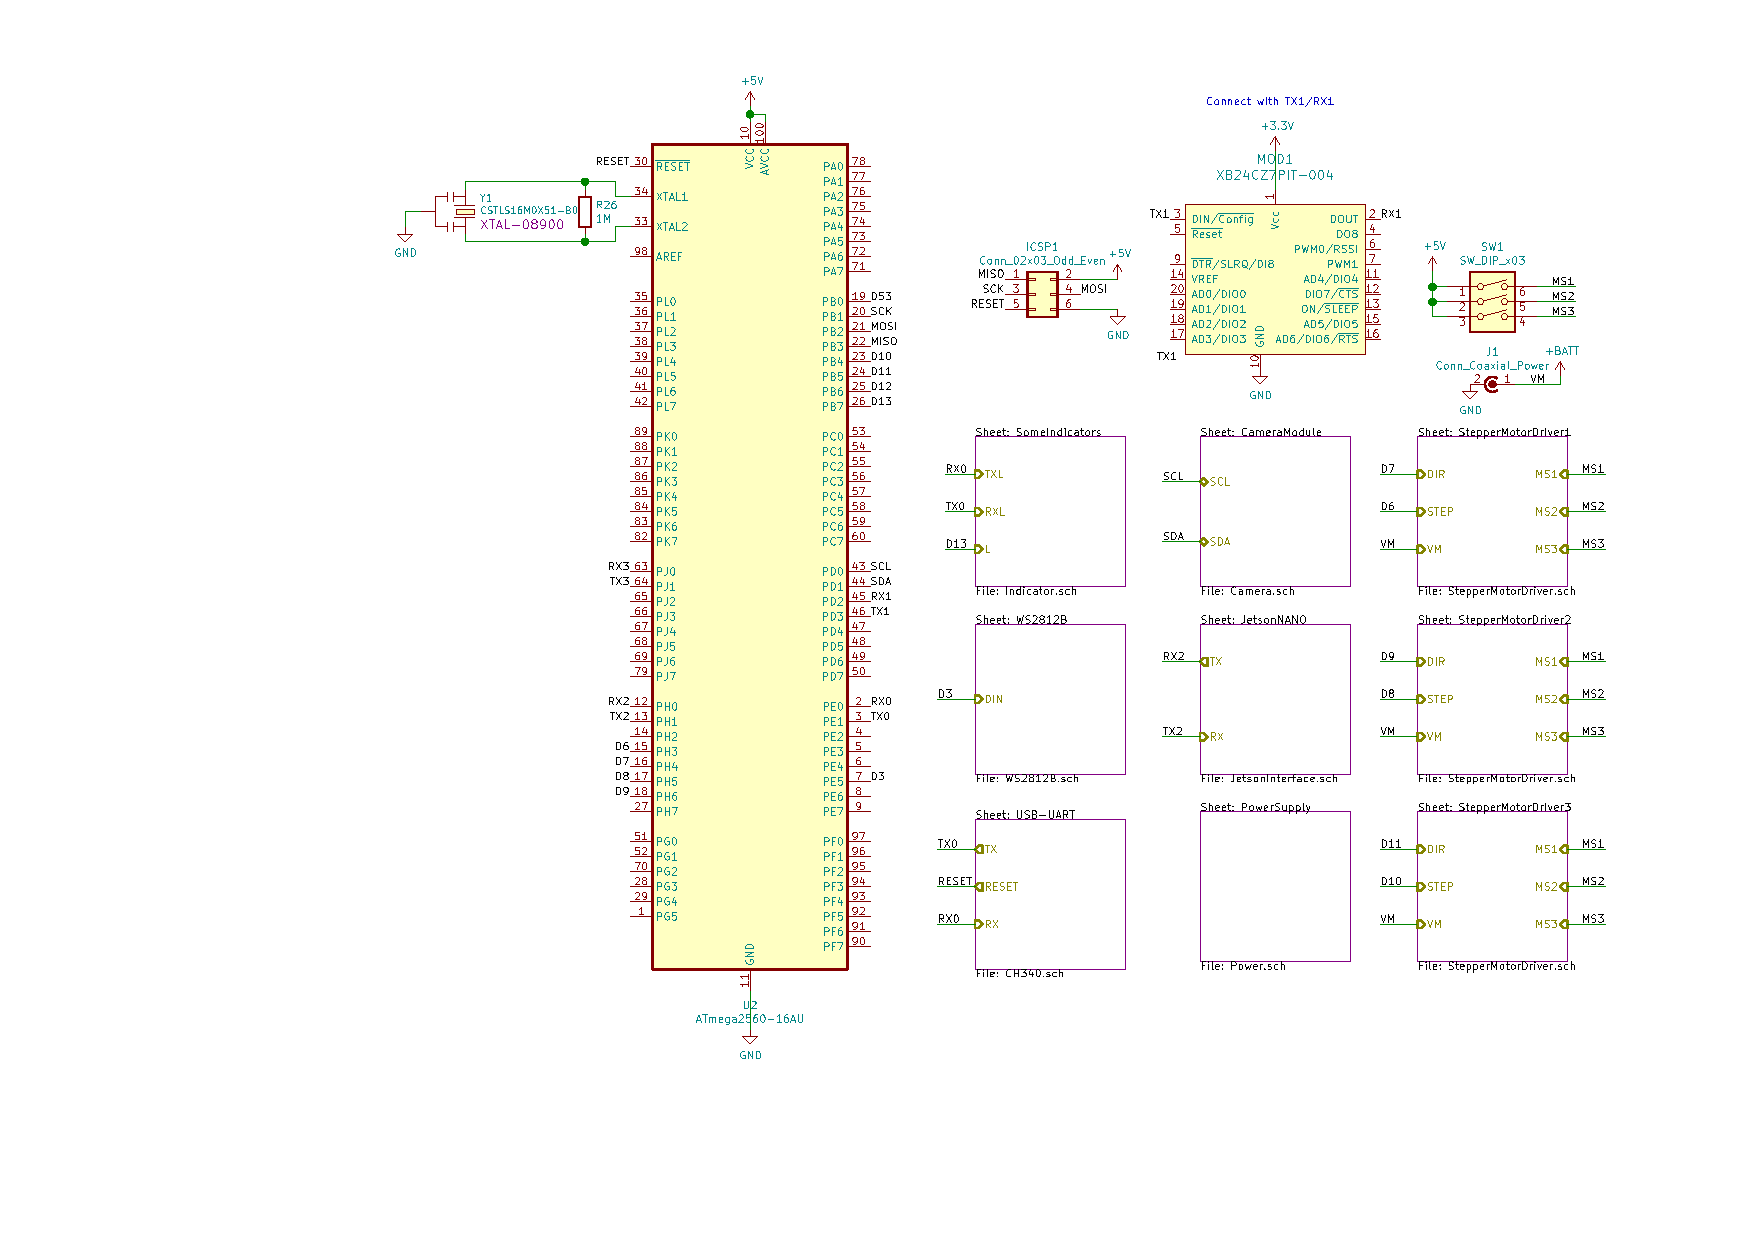
\includegraphics[width=\columnwidth]{Circuit-1.pdf}
    \caption{原理图}
    \label{fig:Circuit-1}
\end{figure}

第二版本PCB主要着眼于实际平台机械结构和PCB的配合,考虑到平台外轮廓是120mm直径圆内接正六边形,故将PCB画成100mm直径圆内接正六边形并预留三个固定孔位,对应的电机驱动及接口也对应到电机所在的位置。另外在前一个版本的PCB中存在的问题在这个版本中尽可能予以纠正。变更开发环境为开源软件Kicad。

\section{需要解决的问题}

在测试版本的PCB(PCB v1)中出现了不少经过测试发现的问题,在第二版本中尽可能予以纠正:

\begin{itemize}
    \item ATmega2560的晶振封装无法手焊,而且不在嘉立创基础库里,不方便SMT
    \item PowerSTEP01过于昂贵,而且极难手动贴片。
\end{itemize}

\section{设计环境的更改}

PCB的设计依赖电子设计自动化(英语:Electronic design automation,缩写:EDA)软件。

当初绘制PCB v1时使用的时Altium Designer 20.0.9集成开发环境,如图~\ref{fig:AltiumDesignerInterface}所示。

\begin{figure}[htbp]
    \centering
    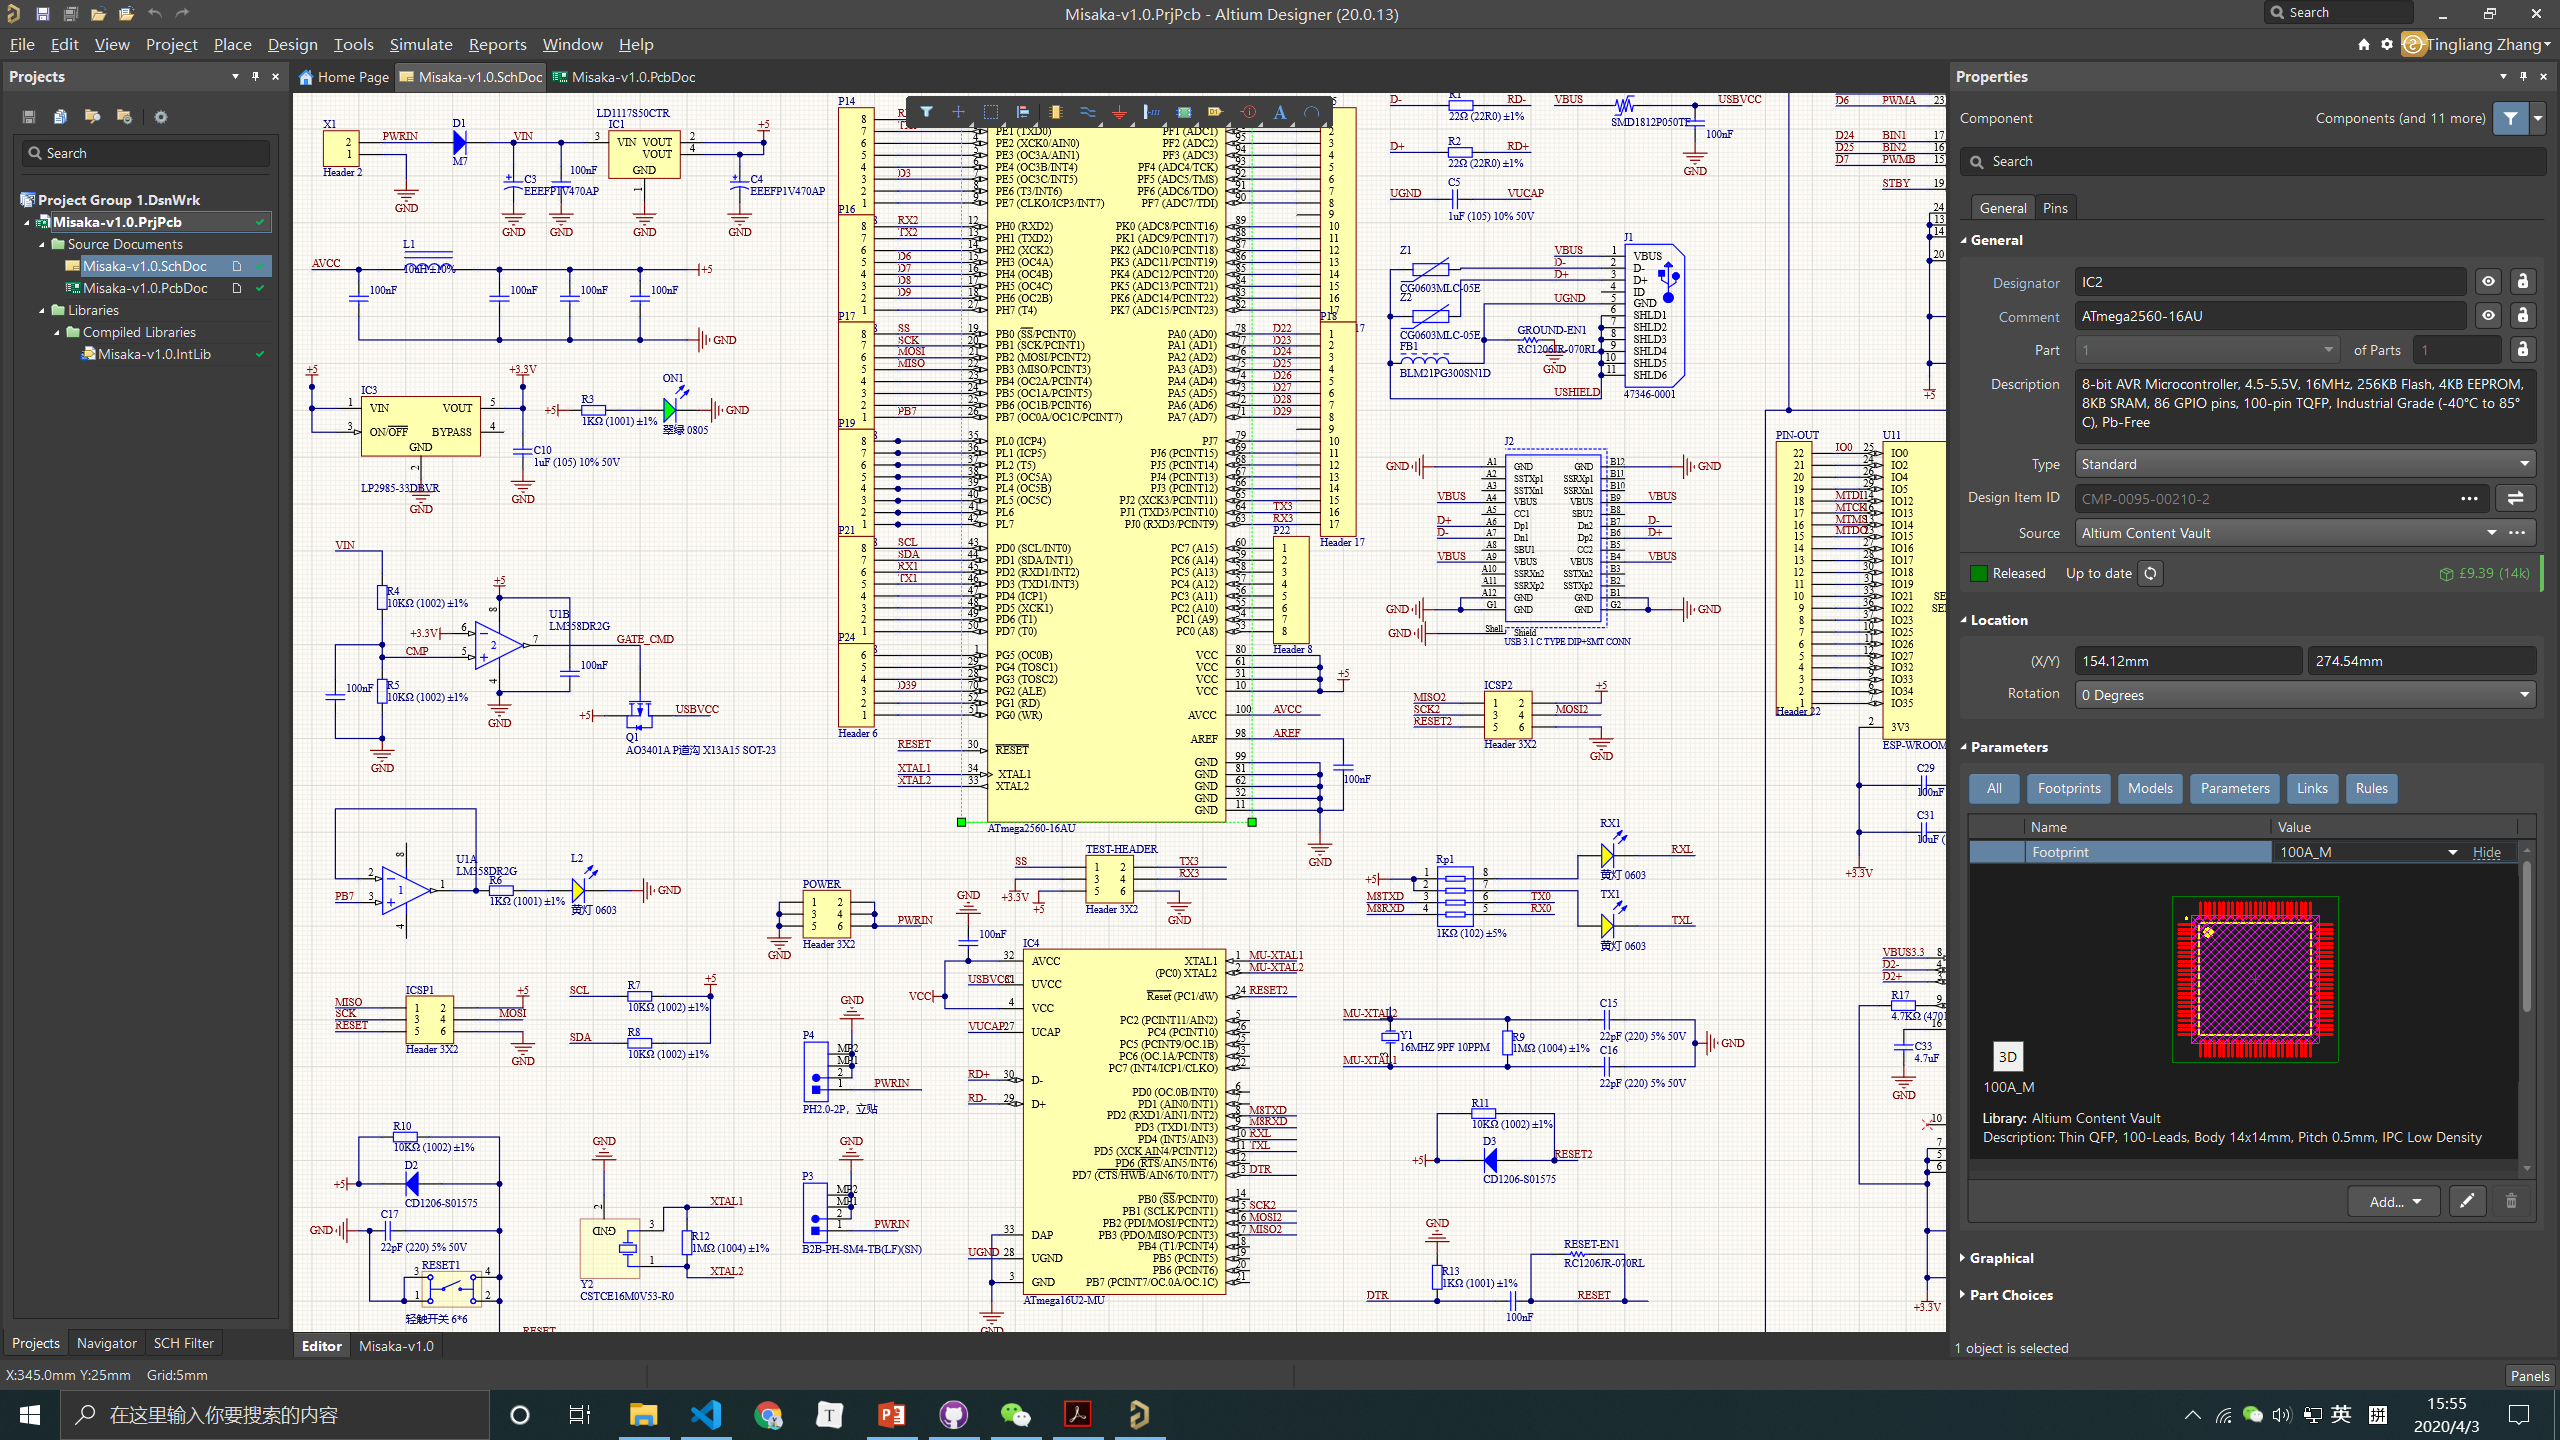
\includegraphics[width=\columnwidth]{AltiumDesignerInterface.png}
    \caption{Altium Designer 20.0.9集成开发环境}
    \label{fig:AltiumDesignerInterface}
\end{figure}

由于AD20是商业付费EDA软件,而且之前的绘制使用了Altium Live 在线供应商封装库,可移植性和便携性不是很好,即使生成了Integrated Library,也很难找到成套的规范化封装。另外AD20的源文件不是普通编辑器可以打开的文本,这使得Git代码管理变得困难。

基于以上考量,改用KiCAD开源EDA软件进行目前及将来的电路设计,

KiCAD界面如图~\ref{fig:KiCAD-Interface}所示。

\begin{figure}[htbp]
    \centering
    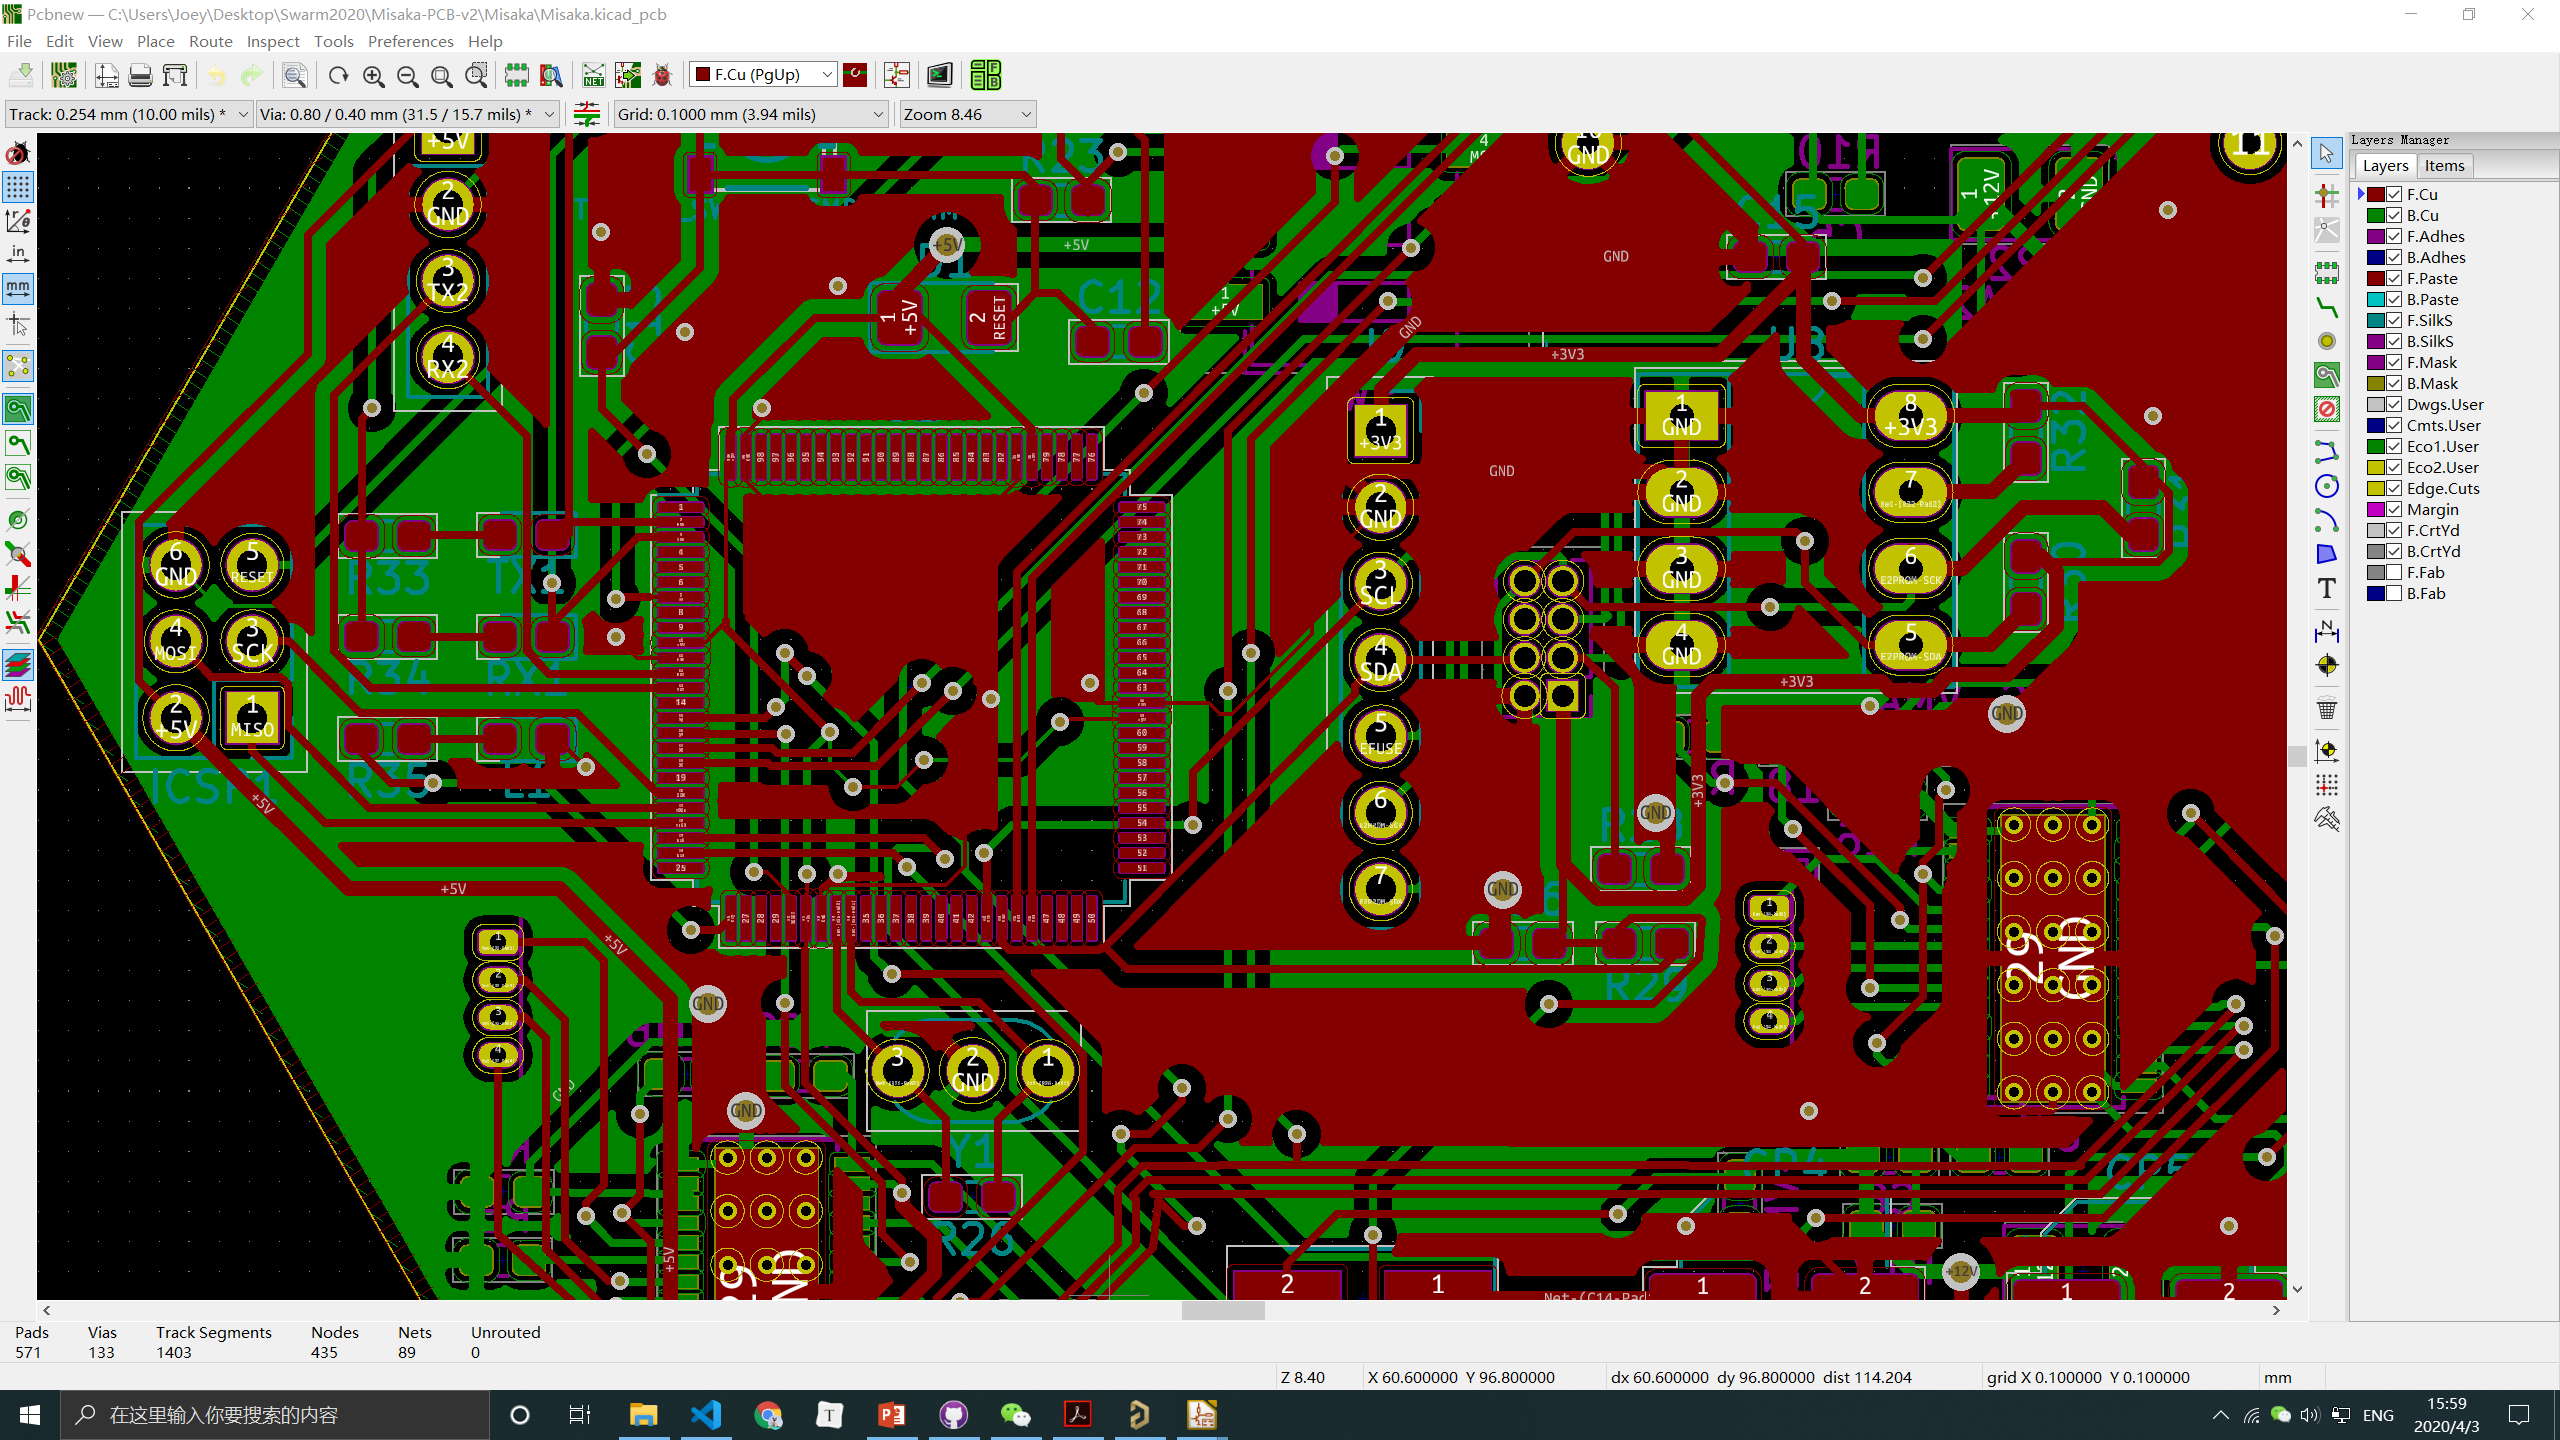
\includegraphics[width=\columnwidth]{KiCAD-Interface.png}
    \caption{KiCAD开源EDA软件}
    \label{fig:KiCAD-Interface}
\end{figure}

工作流程如图~\ref{fig:kicad_flowchart}。

\begin{figure}[htbp]
    \centering
    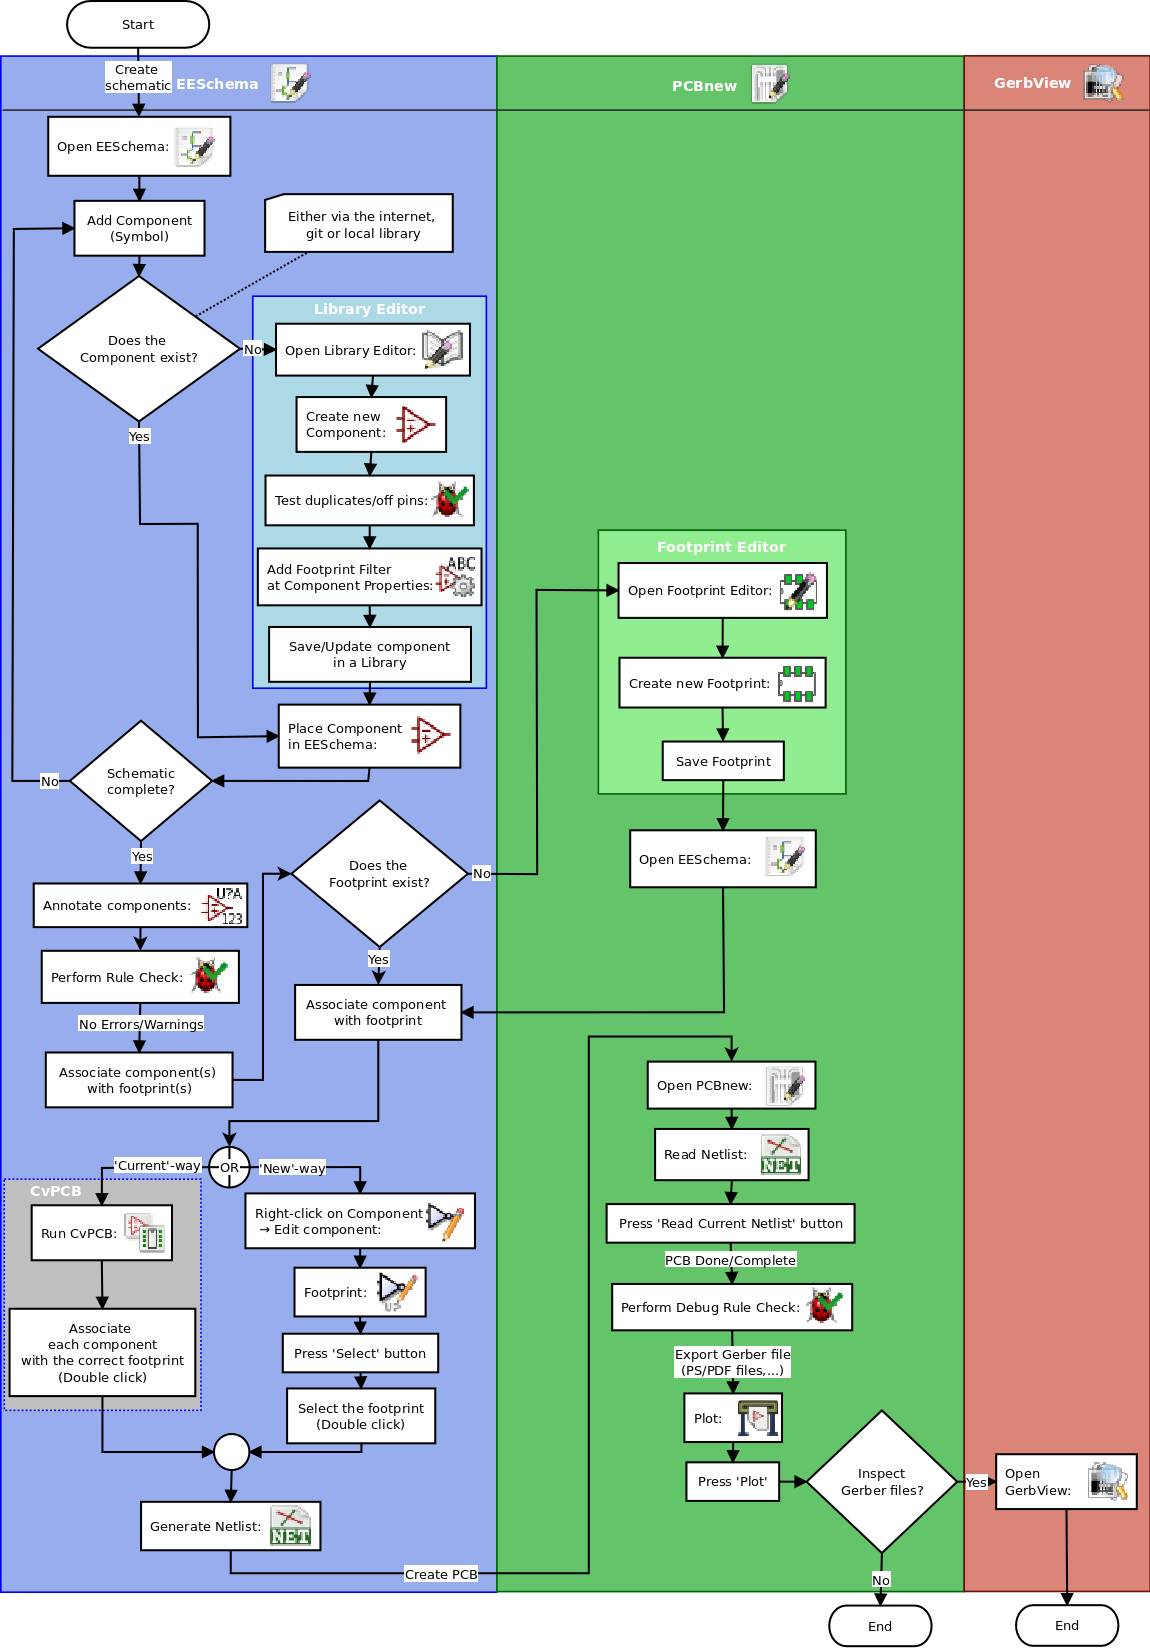
\includegraphics[width=\columnwidth]{kicad_flowchart.png}
    \caption{KiCad Workflow}
    \label{fig:kicad_flowchart}
\end{figure}

新的原理图按照分模块绘制的原则,各模块可复用。

\section{MCU}

本部分原理图如图~\ref{fig:Circuit-1}所示。其中ICSP接口可以使用ISP编程器对第一次使用的MCU烧写固件。

参考了Mega Pro Embed CH340G / ATmega2560 board \footnote{\url{https://robotdyn.com/mega-2560-pro-embed-ch340g-atmega2560-16au.html}}的设计,如图~\ref{fig:MEGA-PRO-CH340GATmega2560}。

\begin{figure}[htbp]
    \centering
    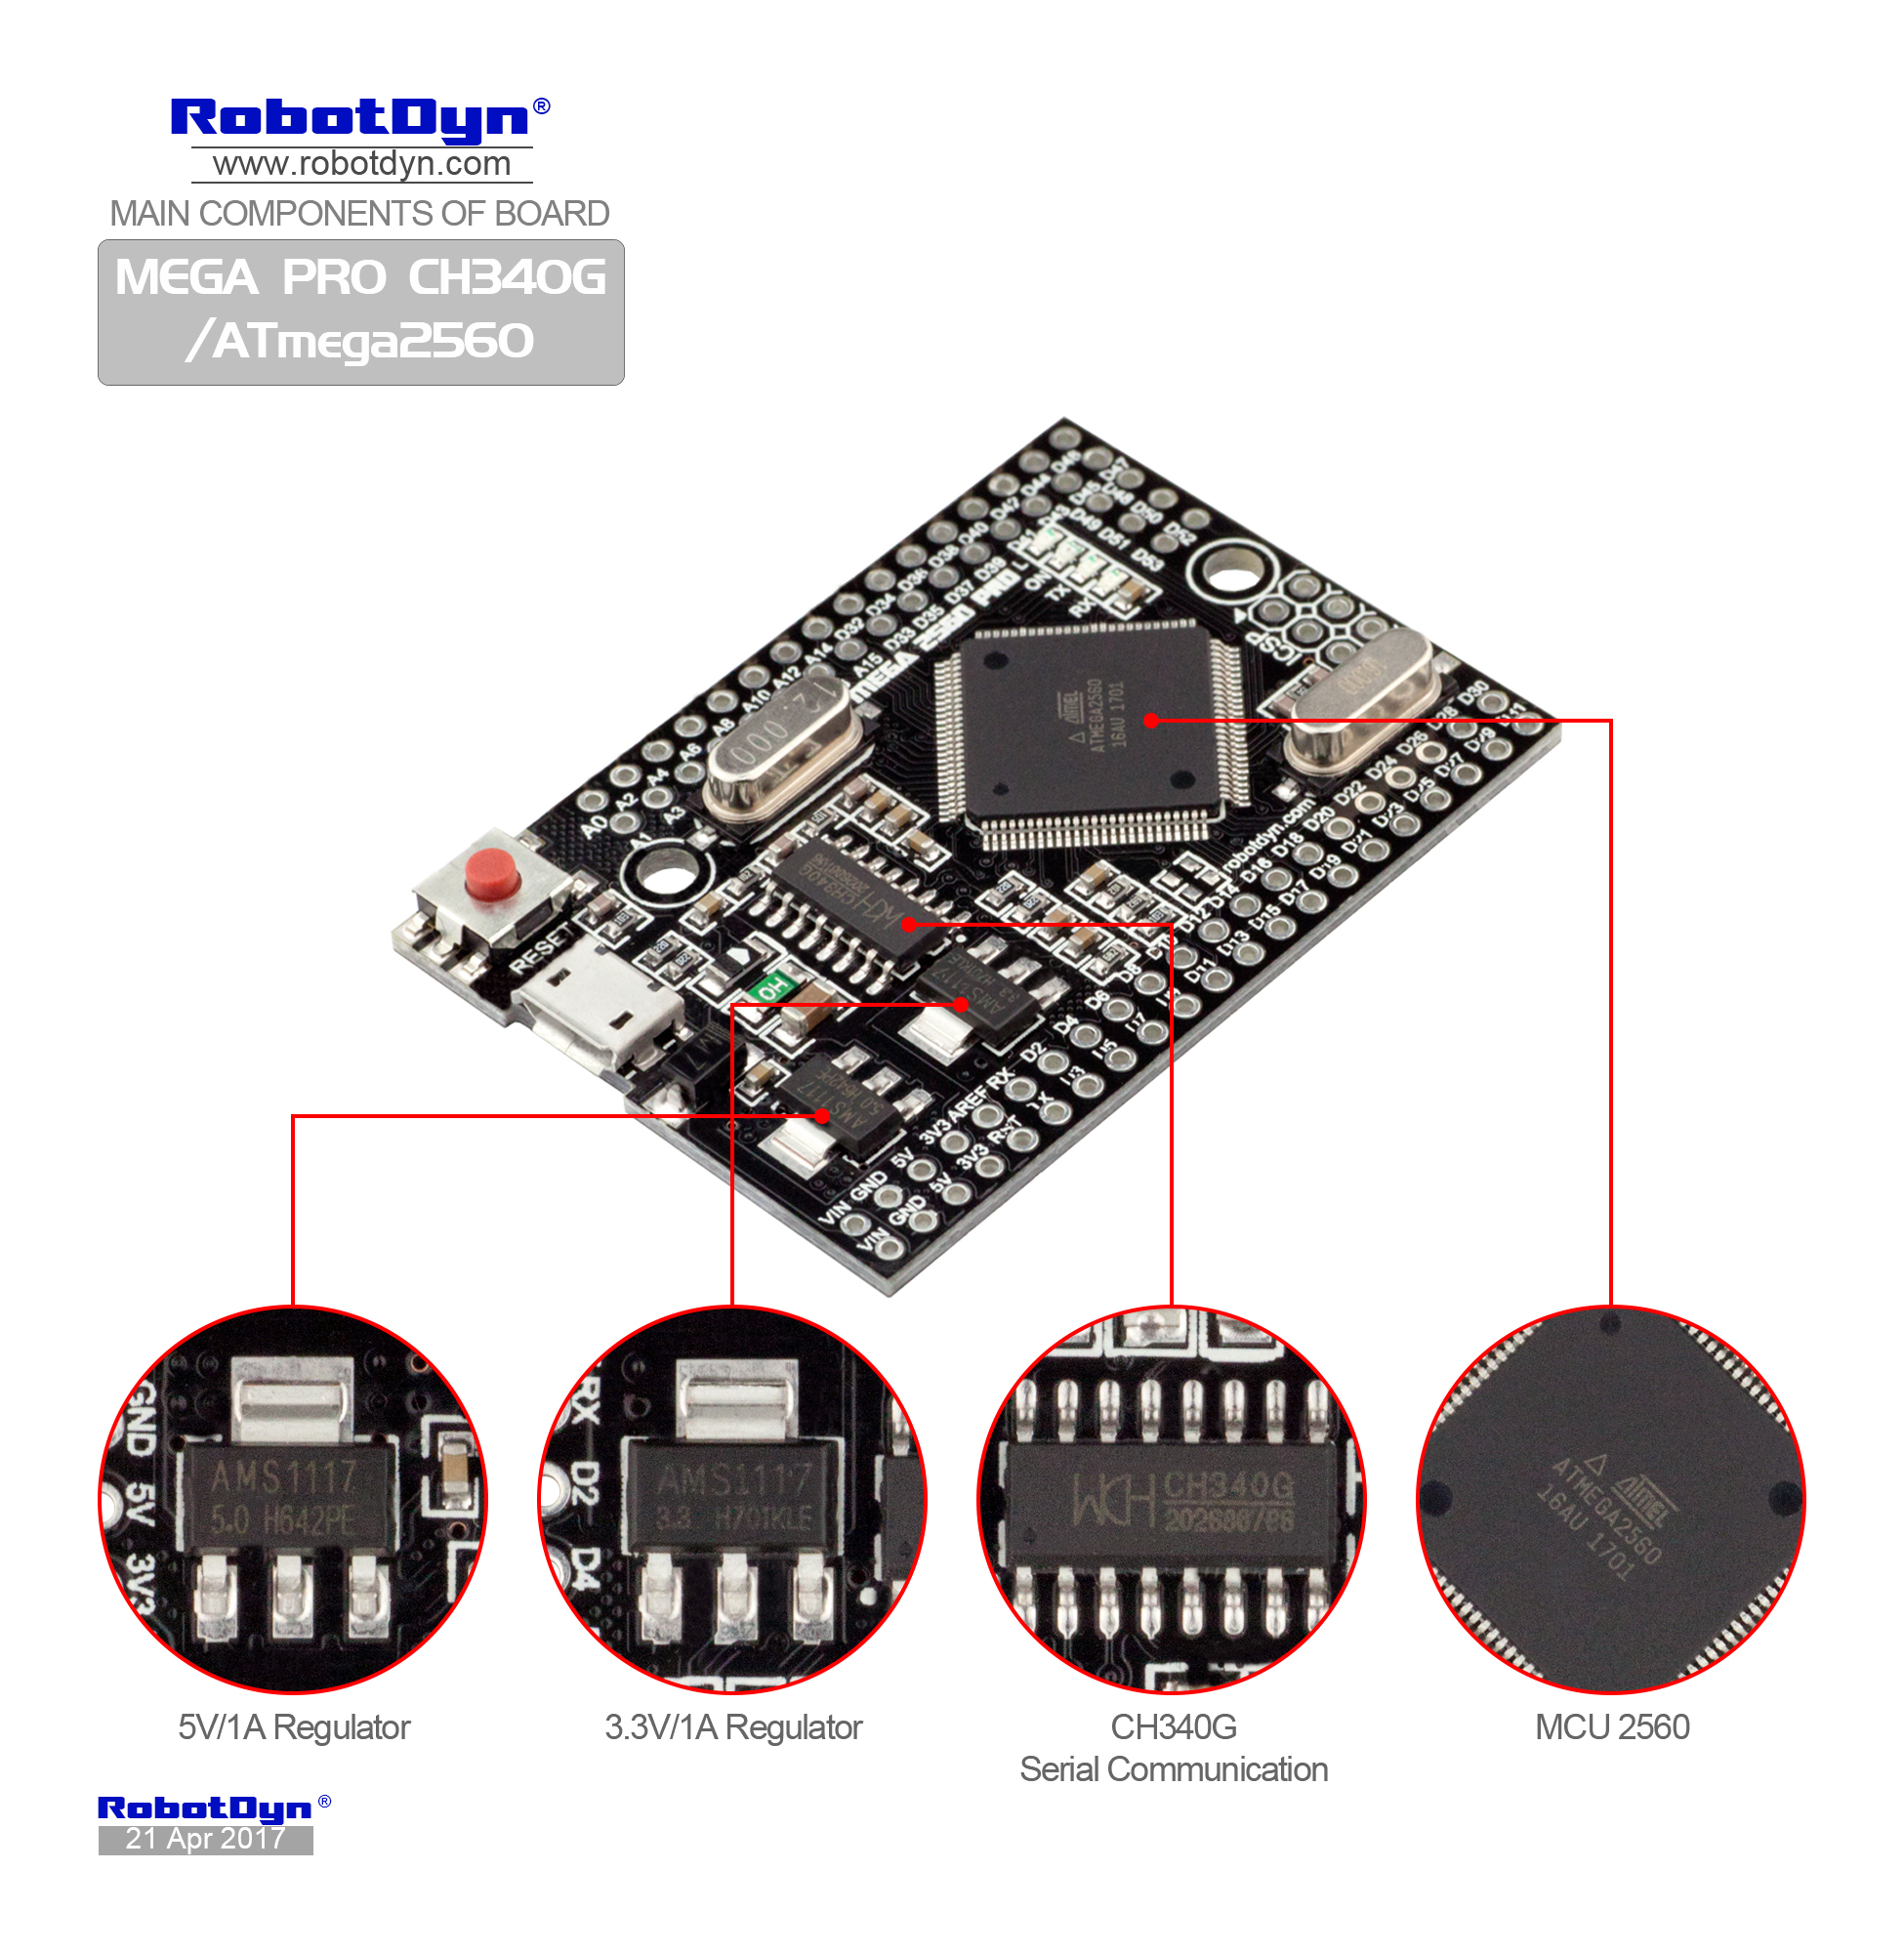
\includegraphics[width=\columnwidth]{MEGA-PRO-CH340GATmega2560.jpg}
    \caption{Mega Pro Embed CH340G / ATmega2560}
    \label{fig:MEGA-PRO-CH340GATmega2560}
\end{figure}


\section{晶振}

由于陶瓷谐振器大多需要外加电容,且封装很难拿手焊,所以选用陶瓷振荡子。

MURATA的 CSTLS16M0X51-A0 \footnote{\url{https://www.murata.com/zh-cn/products/productdetail?partno=CSTLS16M0X51-B0}}。

村田的CSTLS系列陶瓷振荡子(CERALOCK)特征如下:

\begin{enumerate}
    \item 无需外部负载电容器即可构建振荡电路。系列产品拥有内置电容值各不相同的各种型号,可适用于各种集成电路。
    \item 在宽温度范围内稳定。
    \item 结构小巧、重量轻并表现出优异的耐冲击性能。
    \item 可以设计用无需调校的振荡器电路
    \item 性价比高,可用性可靠。
\end{enumerate}

\section{XBee}

XBee模块通过TX1/RX1和MCU连接,如图~\ref{fig:Circuit-1}所示。

XBee模块的底座是两排1x10 Pitch = 2mm 的母排。

\section{USB UART 异步串行数据传输芯片}

USB转UART芯片稳定程度和价格均为FT232>CH340>PL2303。

FT232RL-REEL价格最贵,1片要27.61,1000+批量价格也要16.24每个。FT232RL/BL的优势就FTDI一直在更新驱动发布在官网,驱动经过微软认证,兼容性最好。内部固化了USB底层协议,转出来的是虚拟串口,可以固定COM口号。电路简单,数据传输稳定性好。FT232RL自带晶振,可以转RS232/TTL(常用)及RS422,RS485 高端市场专用。

PL2303最便宜,但波特率在115200时就有可能出现延迟。

经过测试,CH340\footnote{\url{http://www.wch.cn/products/CH340.html}}可以满足需求,且批量购买1000+只要1.47一片。

CH340C内置晶振,最为合适。

下图是统一供电方式下MCU 单片机通过TTL 串口连接CH340 芯片实现USB通讯的参考电路。该产品选择自供电方式,VCC 支持5V 或者3.3V(VCC 为3.3V 时V3 需短接到VCC),完全不使用USB 总线电源VBUS(如有需要MCU可以通过I/O 串电阻后检测其是否有效)。CH340 与MCU 使用同一电源VCC,所以CH340与MCU 之间不存在双电源通过I/O相互电流倒灌的情形。

CH340没有使用到的信号线都可以悬空。对于CH340C/N/K/E/B 芯片,无需X6 和C17 及C18。

CH340C原理图如图~\ref{fig:Circuit-10}所示。

\begin{figure}[htbp]
    \centering
    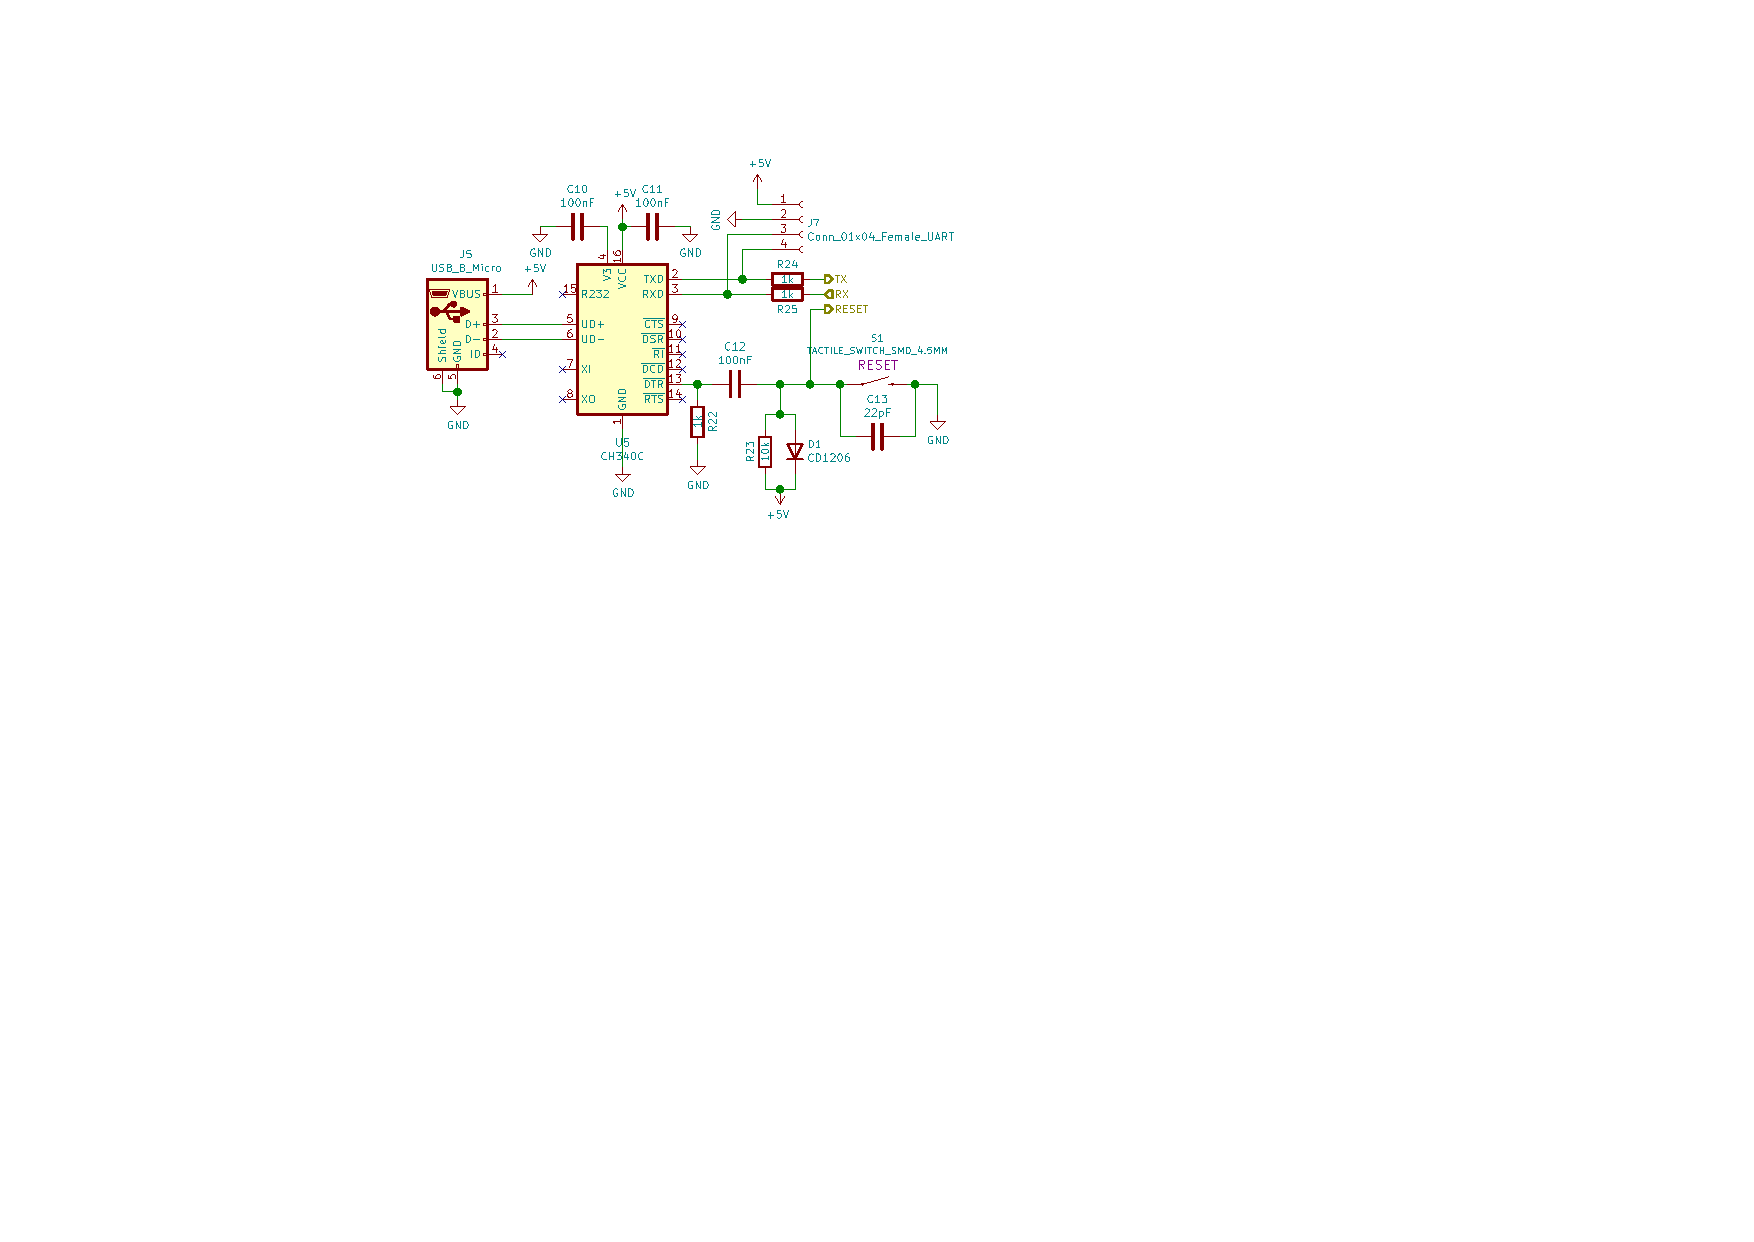
\includegraphics[width=\columnwidth]{Circuit-10.pdf}
    \caption{CH340C原理图}
    \label{fig:Circuit-10}
\end{figure}

除了常规的USB转UART电路之外,还在DTR端口引出了MCU的RESET功能,每次烧写完成后自动RESET MCU。

\section{电机驱动}

电机驱动模块原理图如图~\ref{fig:Circuit-2}所示。

\begin{figure}[htbp]
    \centering
    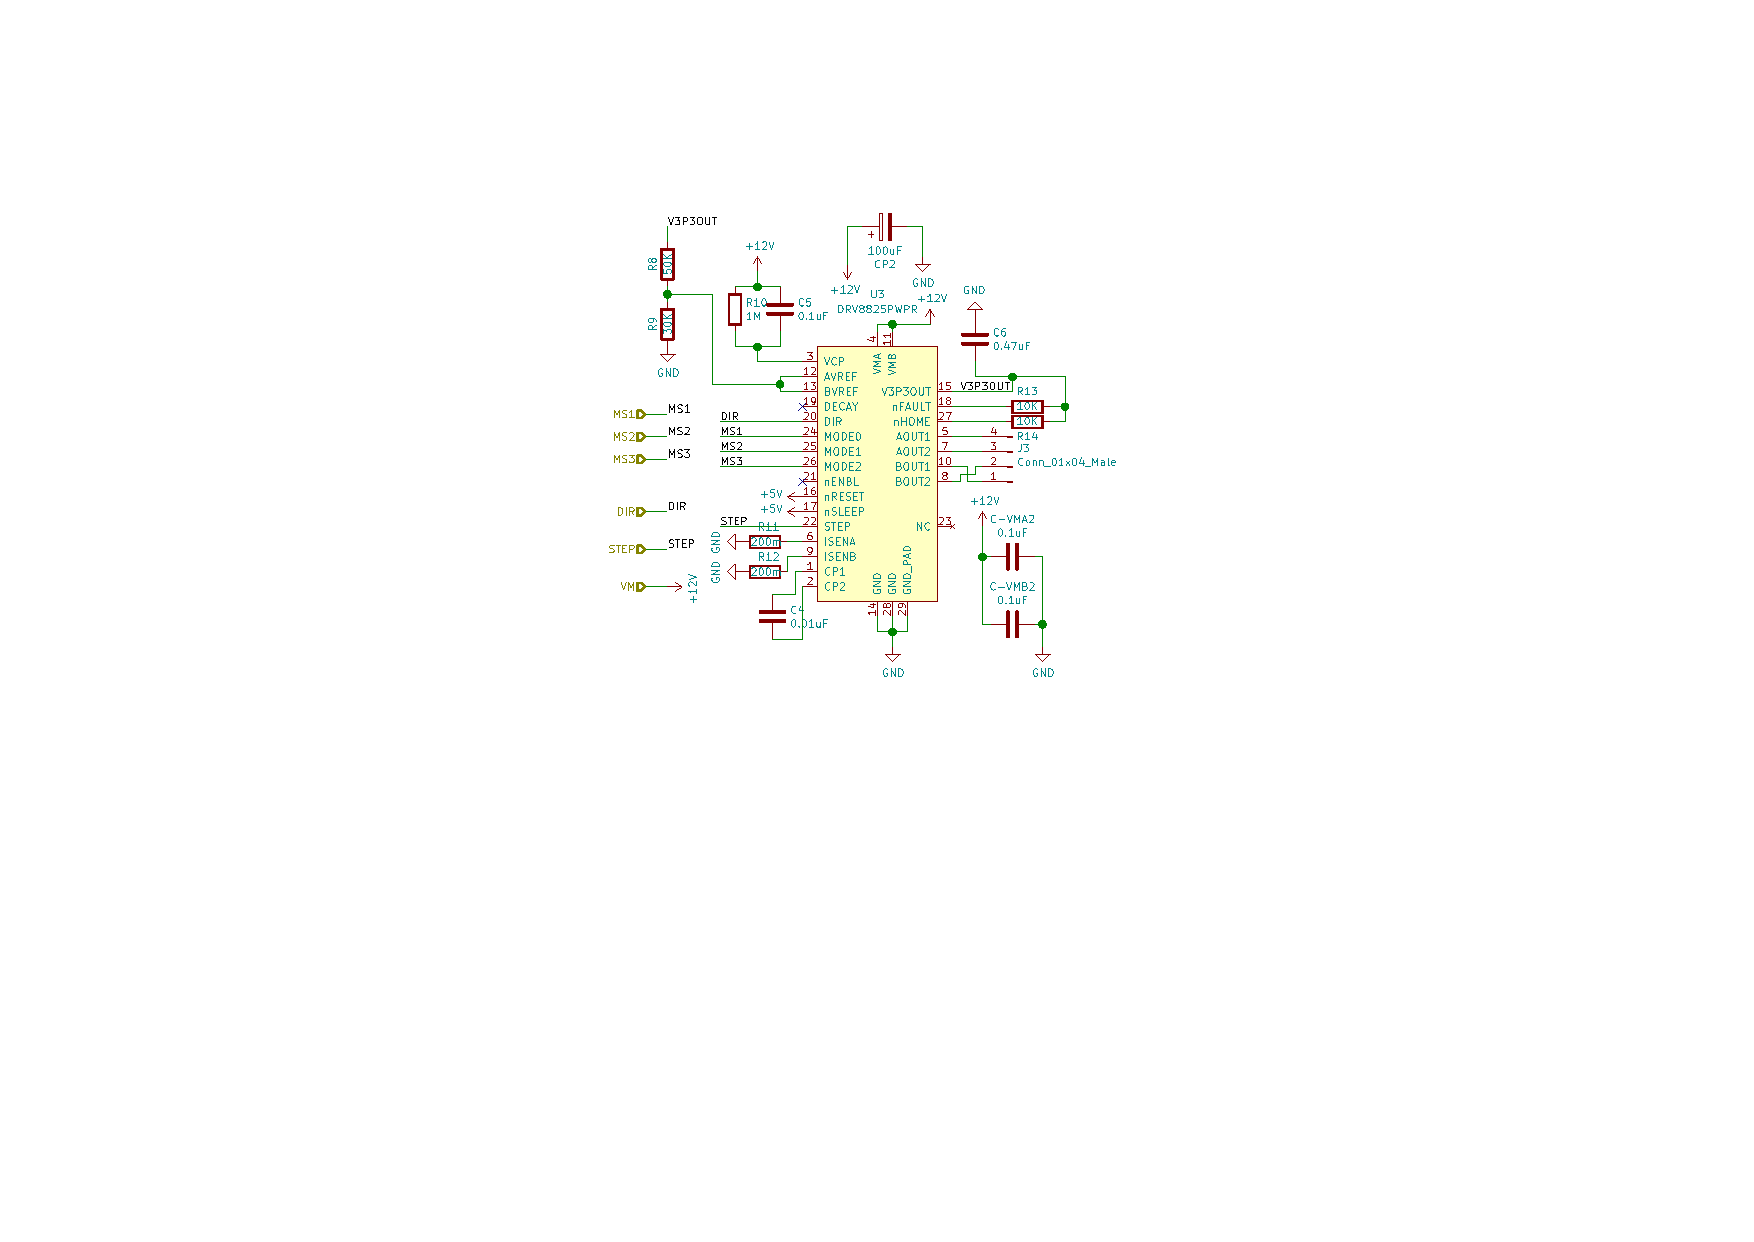
\includegraphics[width=\columnwidth]{Circuit-2.pdf}
    \caption{电机驱动模块原理图}
    \label{fig:Circuit-2}
\end{figure}

其中,MS1-3可以用来选择步进模式,由一个拨码开关控制。

AVREF则可以限定电流上限,这里我们先按照单电机128mA计算。之后如果涉及到替换电机,相应的更换电阻即可。

\section{供电}

供电模块原理图如图~\ref{fig:Circuit-5}所示。

\begin{figure}[htbp]
    \centering
    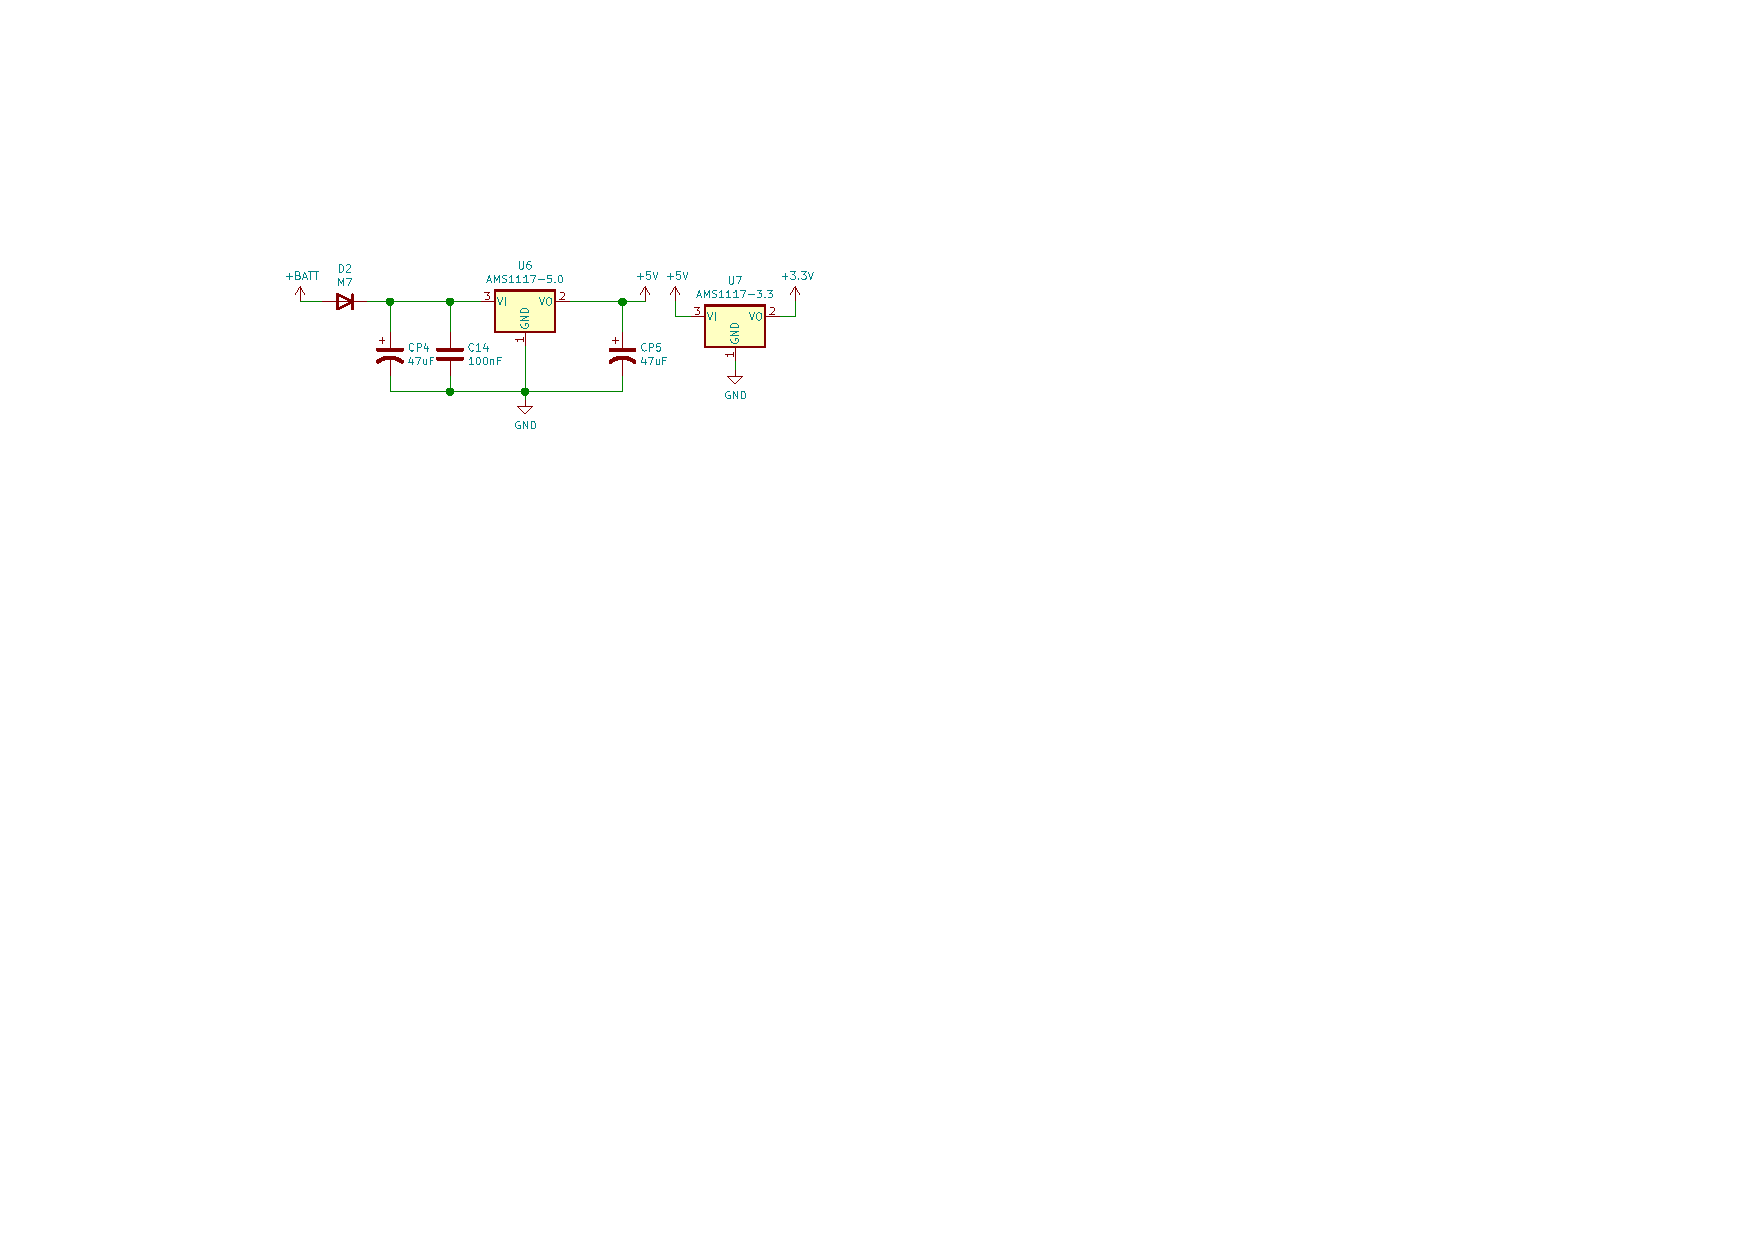
\includegraphics[width=\columnwidth]{Circuit-5.pdf}
    \caption{供电模块原理图}
    \label{fig:Circuit-5}
\end{figure}

使用两片AMS1117芯片将电压从12V降至5V再降至3.3V,以供逻辑电路使用。

之后考虑使用USB PD,比如使用USB PD等多快充协议芯片CH236\footnote{\url{http://www.wch.cn/products/CH236.html}}

\section{Jetson NANO接口}

Jetson NANO接口模块原理图如图~\ref{fig:Circuit-6}所示。

\begin{figure}[htbp]
    \centering
    
\includegraphics[width=0.5\columnwidth]{Circuit-6.pdf}
    \caption{Jetson NANO接口模块原理图}
    \label{fig:Circuit-6}
\end{figure}

预留了一个UART串口用于Jetson NANO和MCU之间的数据交换。

\section{定位相机}

定位相机模块原理图如图~\ref{fig:Circuit-7}所示。

\begin{figure}[htbp]
    \centering
    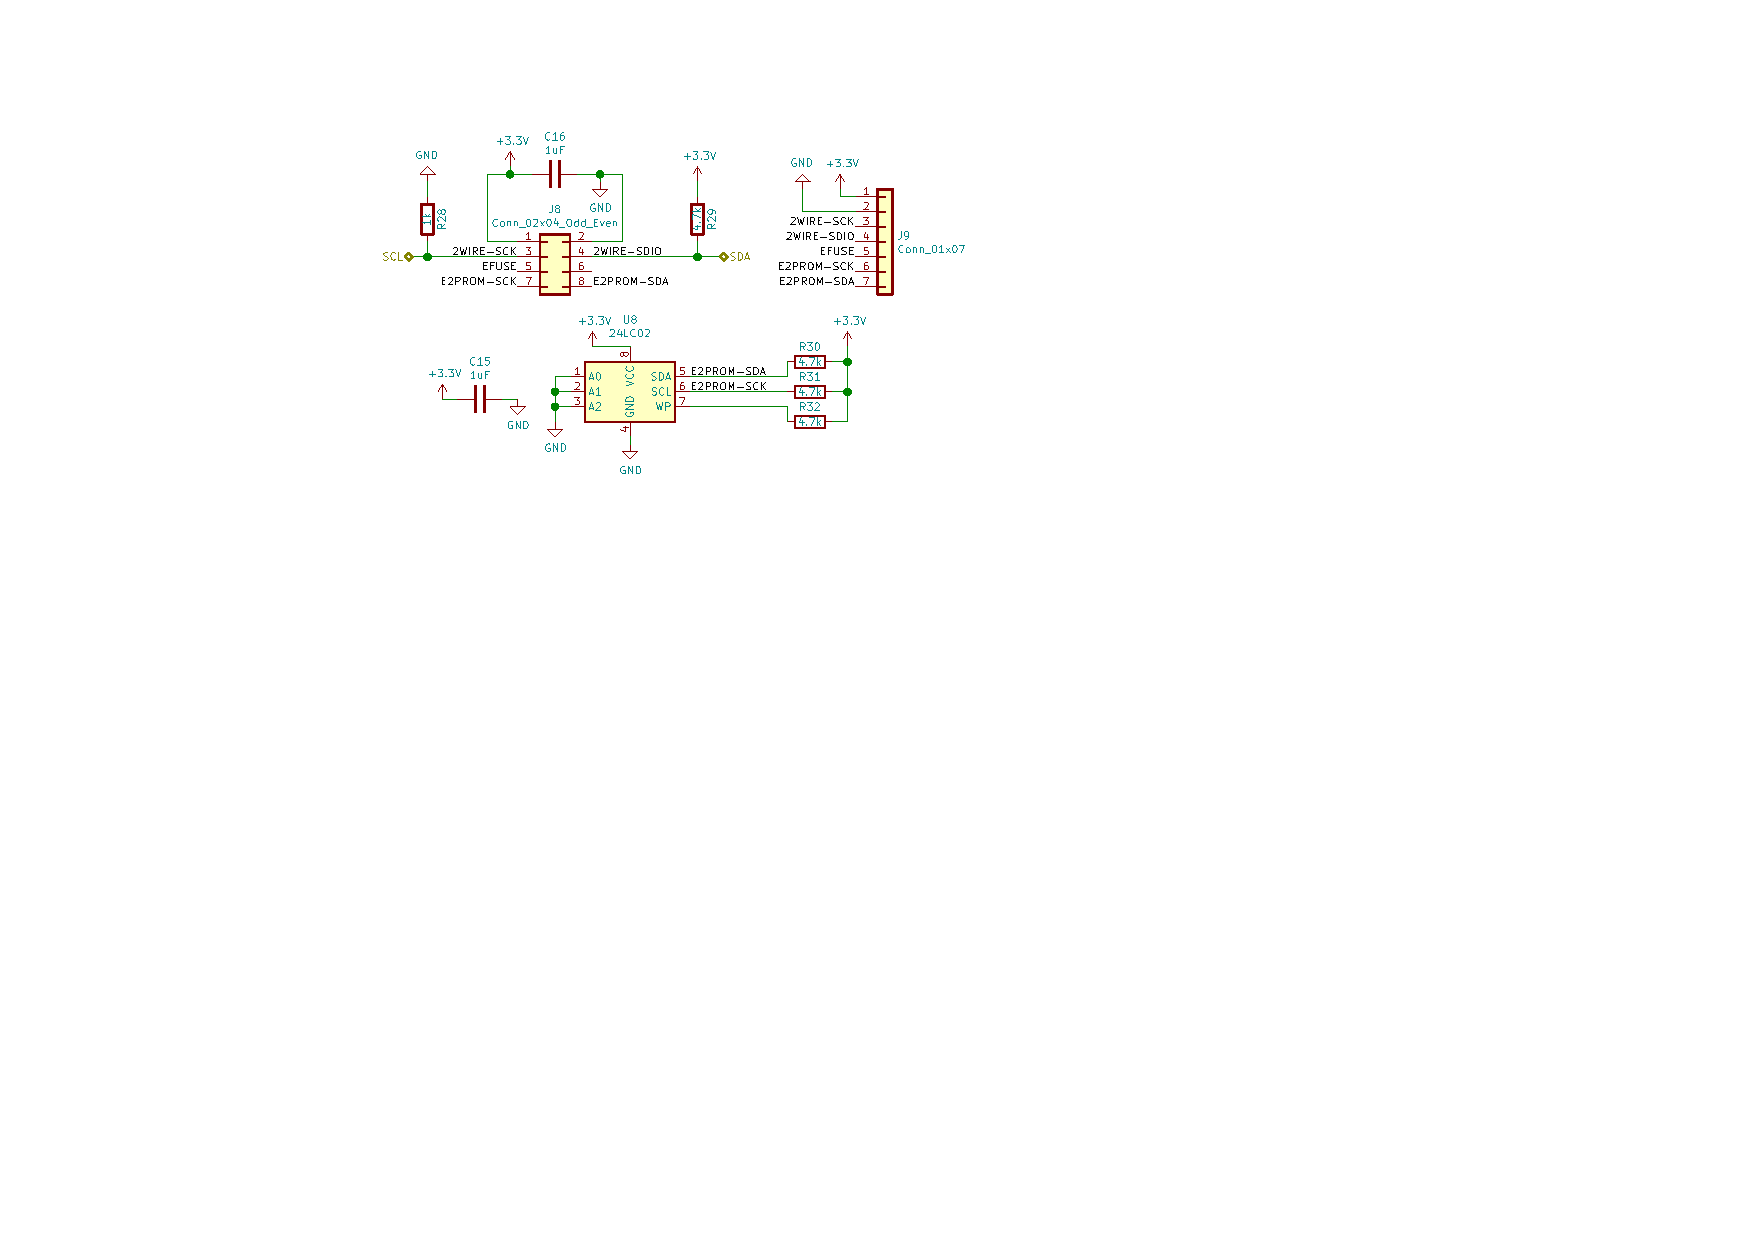
\includegraphics[width=\columnwidth]{Circuit-7.pdf}
    \caption{定位相机模块原理图}
    \label{fig:Circuit-7}
\end{figure}

为了烧写 24LC02 EEPROM 方便,使用DIP-8 EEPROM底座方便取下和安装EEPROM。

特别注意,相机模块的2x4 1.27mm排母需要安装在PCB背面的正中央,以便对准模型中央的孔。

\section{WS2812B}

WS2812B模块原理图如图~\ref{fig:Circuit-8}所示。

\begin{figure}[htbp]
    \centering
    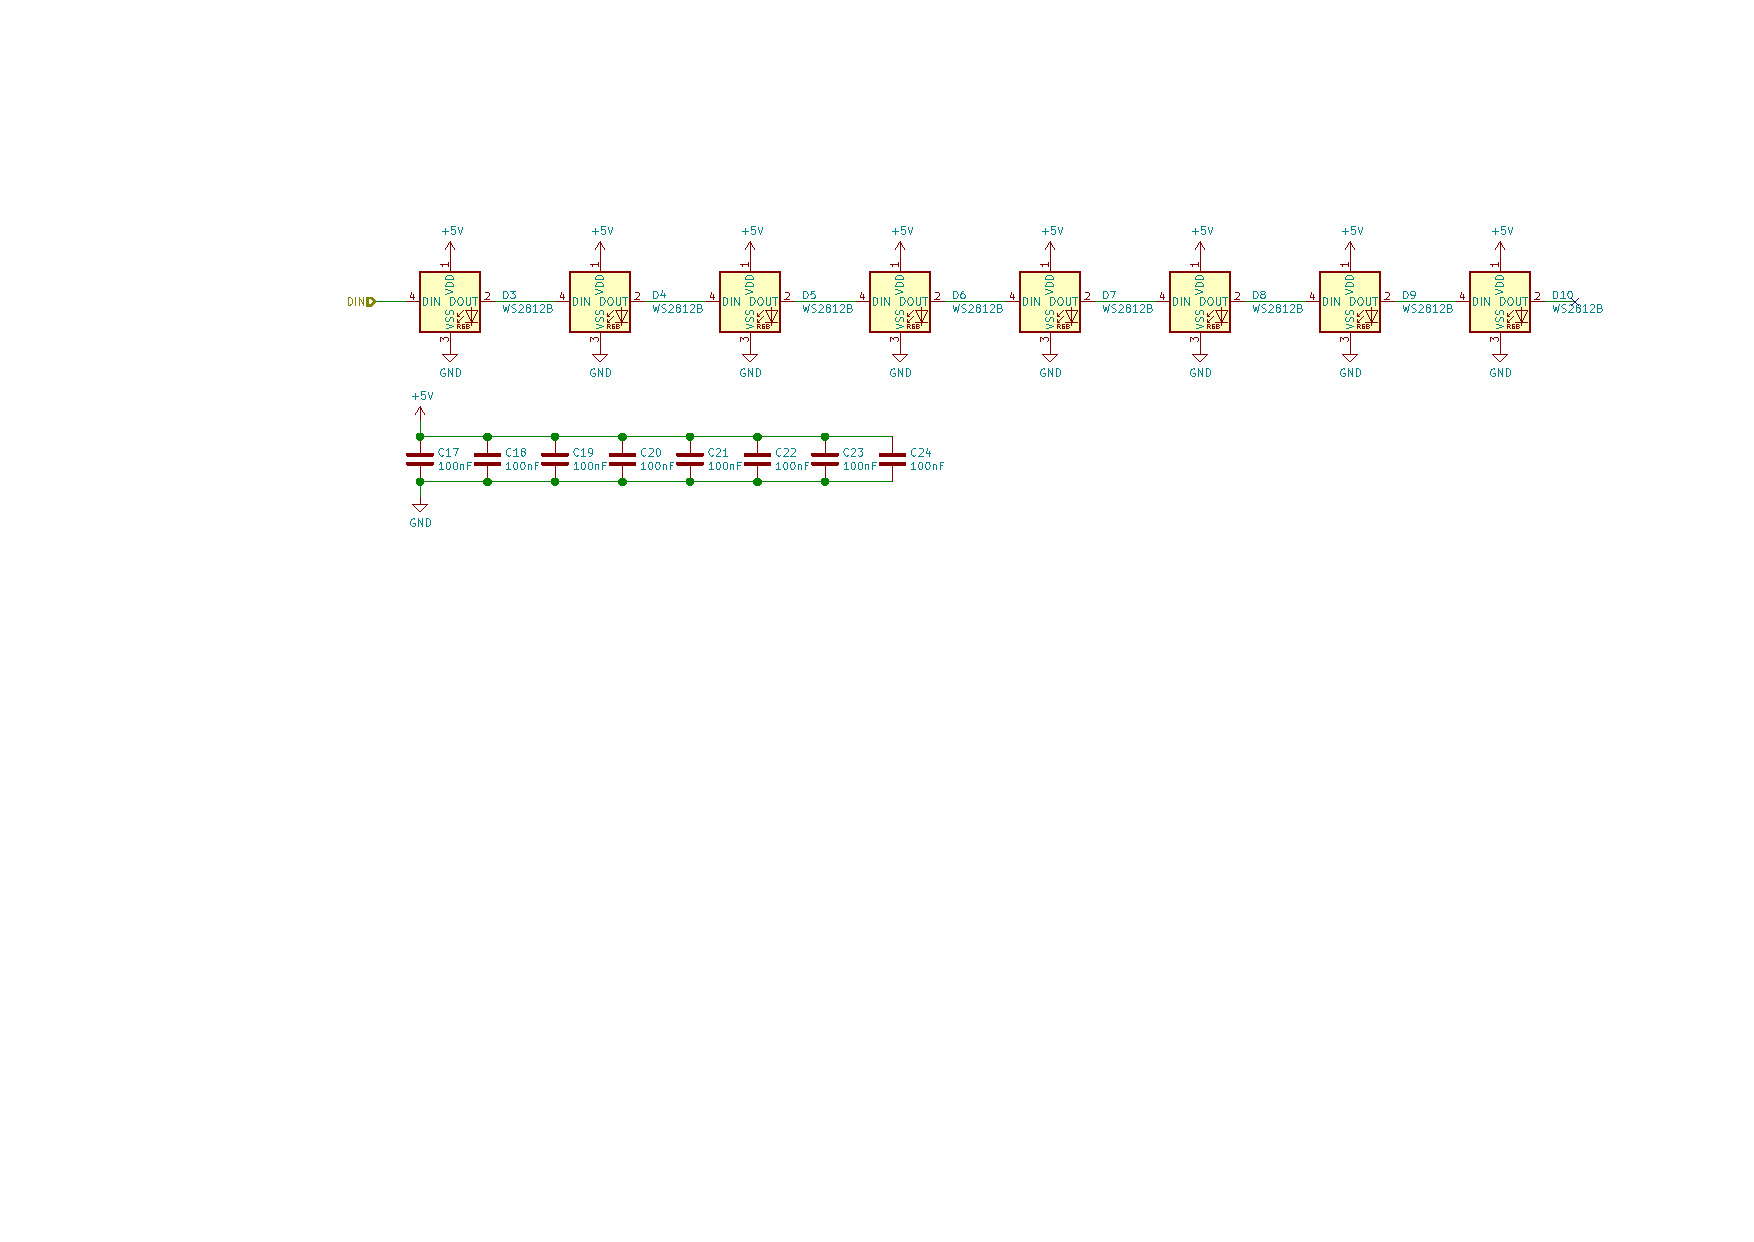
\includegraphics[width=\columnwidth]{Circuit-8.pdf}
    \caption{WS2812B模块原理图}
    \label{fig:Circuit-8}
\end{figure}

定义了8个串联的WS2812B和稳压电容,通过MCU的一个数字引脚控制。

\section{灯光指示}

灯光指示模块原理图如图~\ref{fig:Circuit-9}所示。

\begin{figure}[htbp]
    \centering
    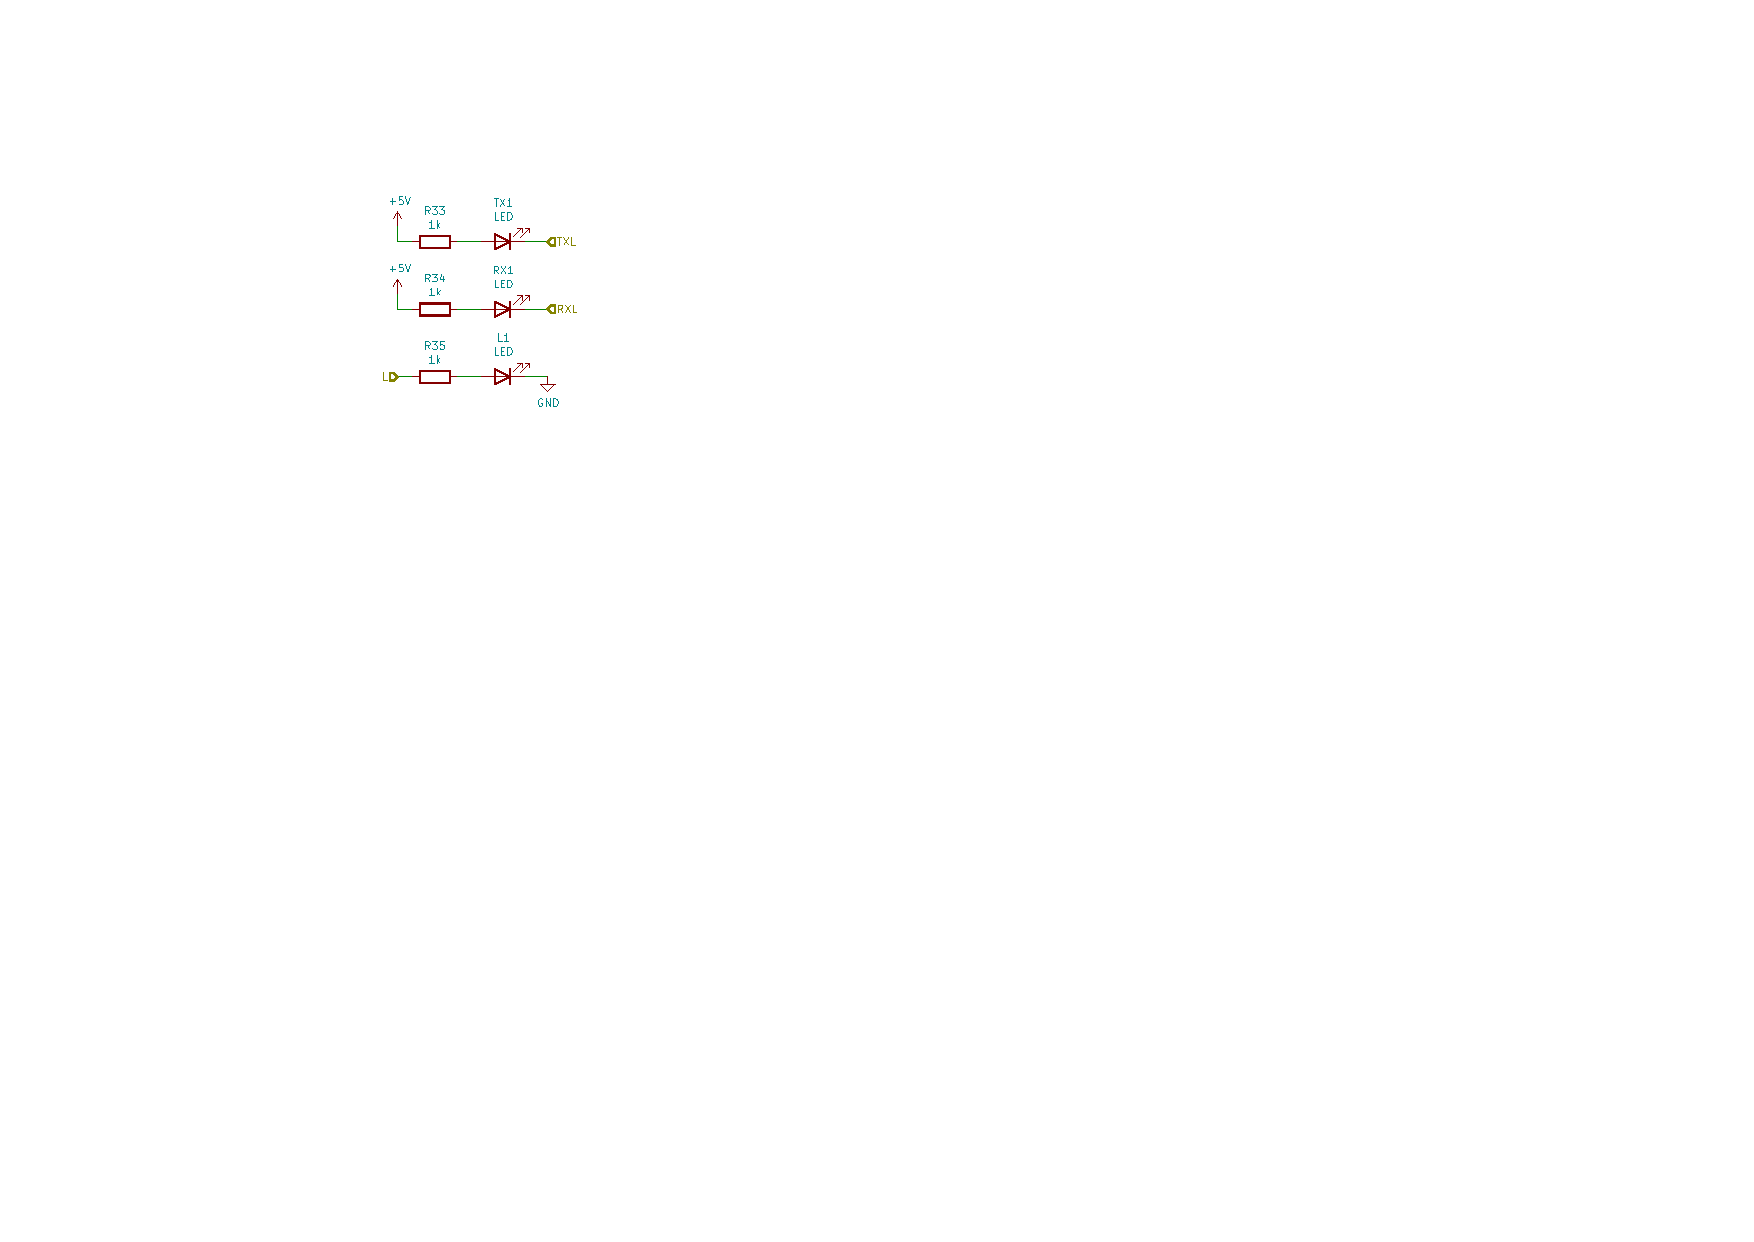
\includegraphics[width=0.5\columnwidth]{Circuit-9.pdf}
    \caption{灯光指示模块原理图}
    \label{fig:Circuit-9}
\end{figure}

定义了三个0603 LED,分别指示烧写TX/RX和D13引脚的电平情况。

\section{定义板子外形轮廓}

在KiCAD PCBNEW编辑器中可以直接在 'Edge.Cuts' 层使用 'Add graphic line or polygon' 定义板子外形轮廓,空格键定义相对坐标原点。

但是只能画简单的直线和圆,而且很麻烦,所以我们使用Fusion 360 导出 DXF 文件定义外形。

如图~\ref{fig:PCB-Measure-v1}。

\begin{figure}[htbp]
    \centering
    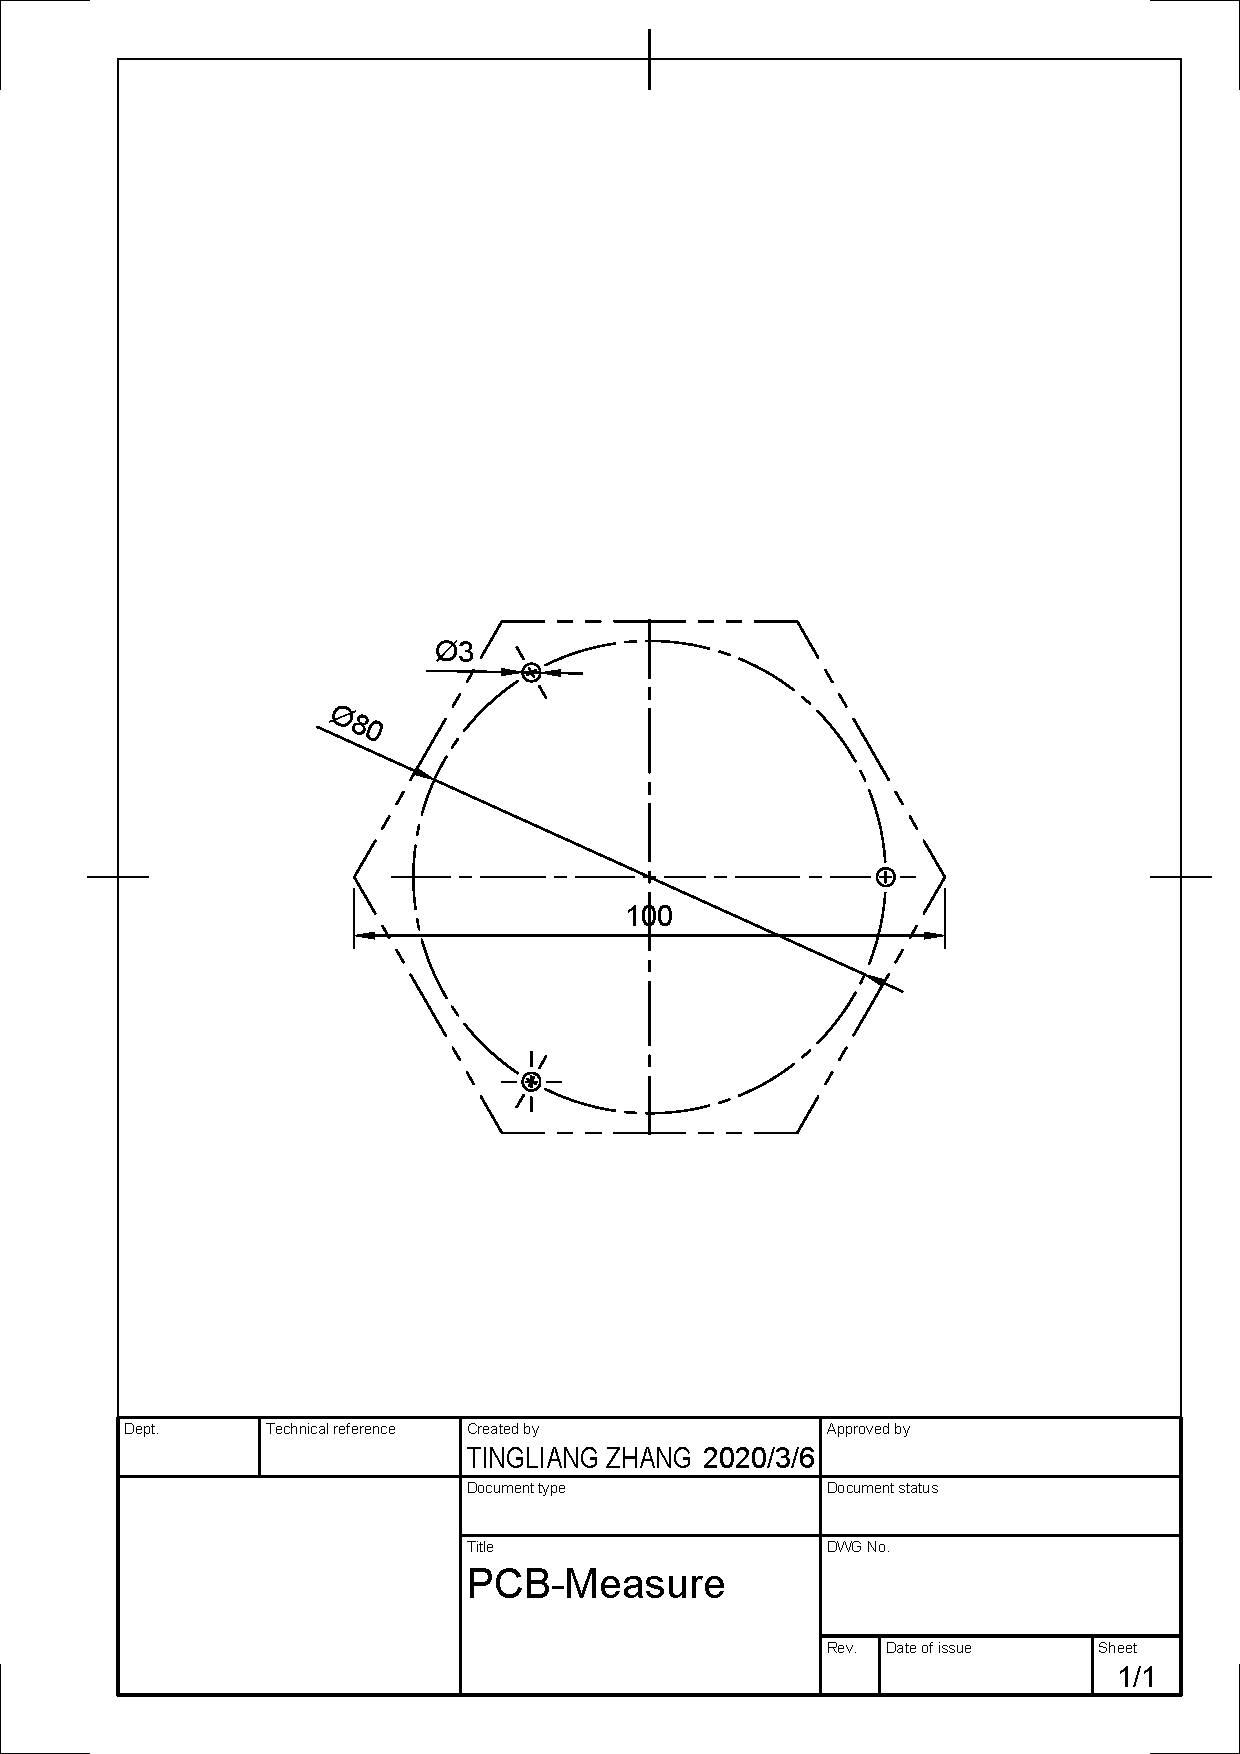
\includegraphics[width=\columnwidth]{PCB-Measure-v1.pdf}
    \caption{PCB DXF}
    \label{fig:PCB-Measure-v1}
\end{figure}


\section{布线}

布线方法参考下文:

Press W or select Custom Track Width from the context menu to type in a custom track width/via size.

To activate the router tool press the Interactive Router button Interactive Router Button or the X key. 

Pressing V or selecting Place Through Via from the context menu while routing a track attaches a via at the end of the trace being routed. Pressing V again disables via placement. Clicking in any spot establishes the via and continues routing (unless 'Shift' is held).

Pressing / or selecting Switch Track Posture from the context menu toggles the direction of the initial track segment between straight or diagonal.

The router can drag track segments, corners and vias. To drag an item, click on it with Ctrl key pressed, hover the mouse and press G or select Drag Track/Via from the context menu.

布线之后的PCB详见附录~\ref{sec:PCB}。

正面如图~\ref{fig:CircuitPCB-F},背面如图~\ref{fig:CircuitPCB-B}。

\begin{figure}[htbp]
    \centering
    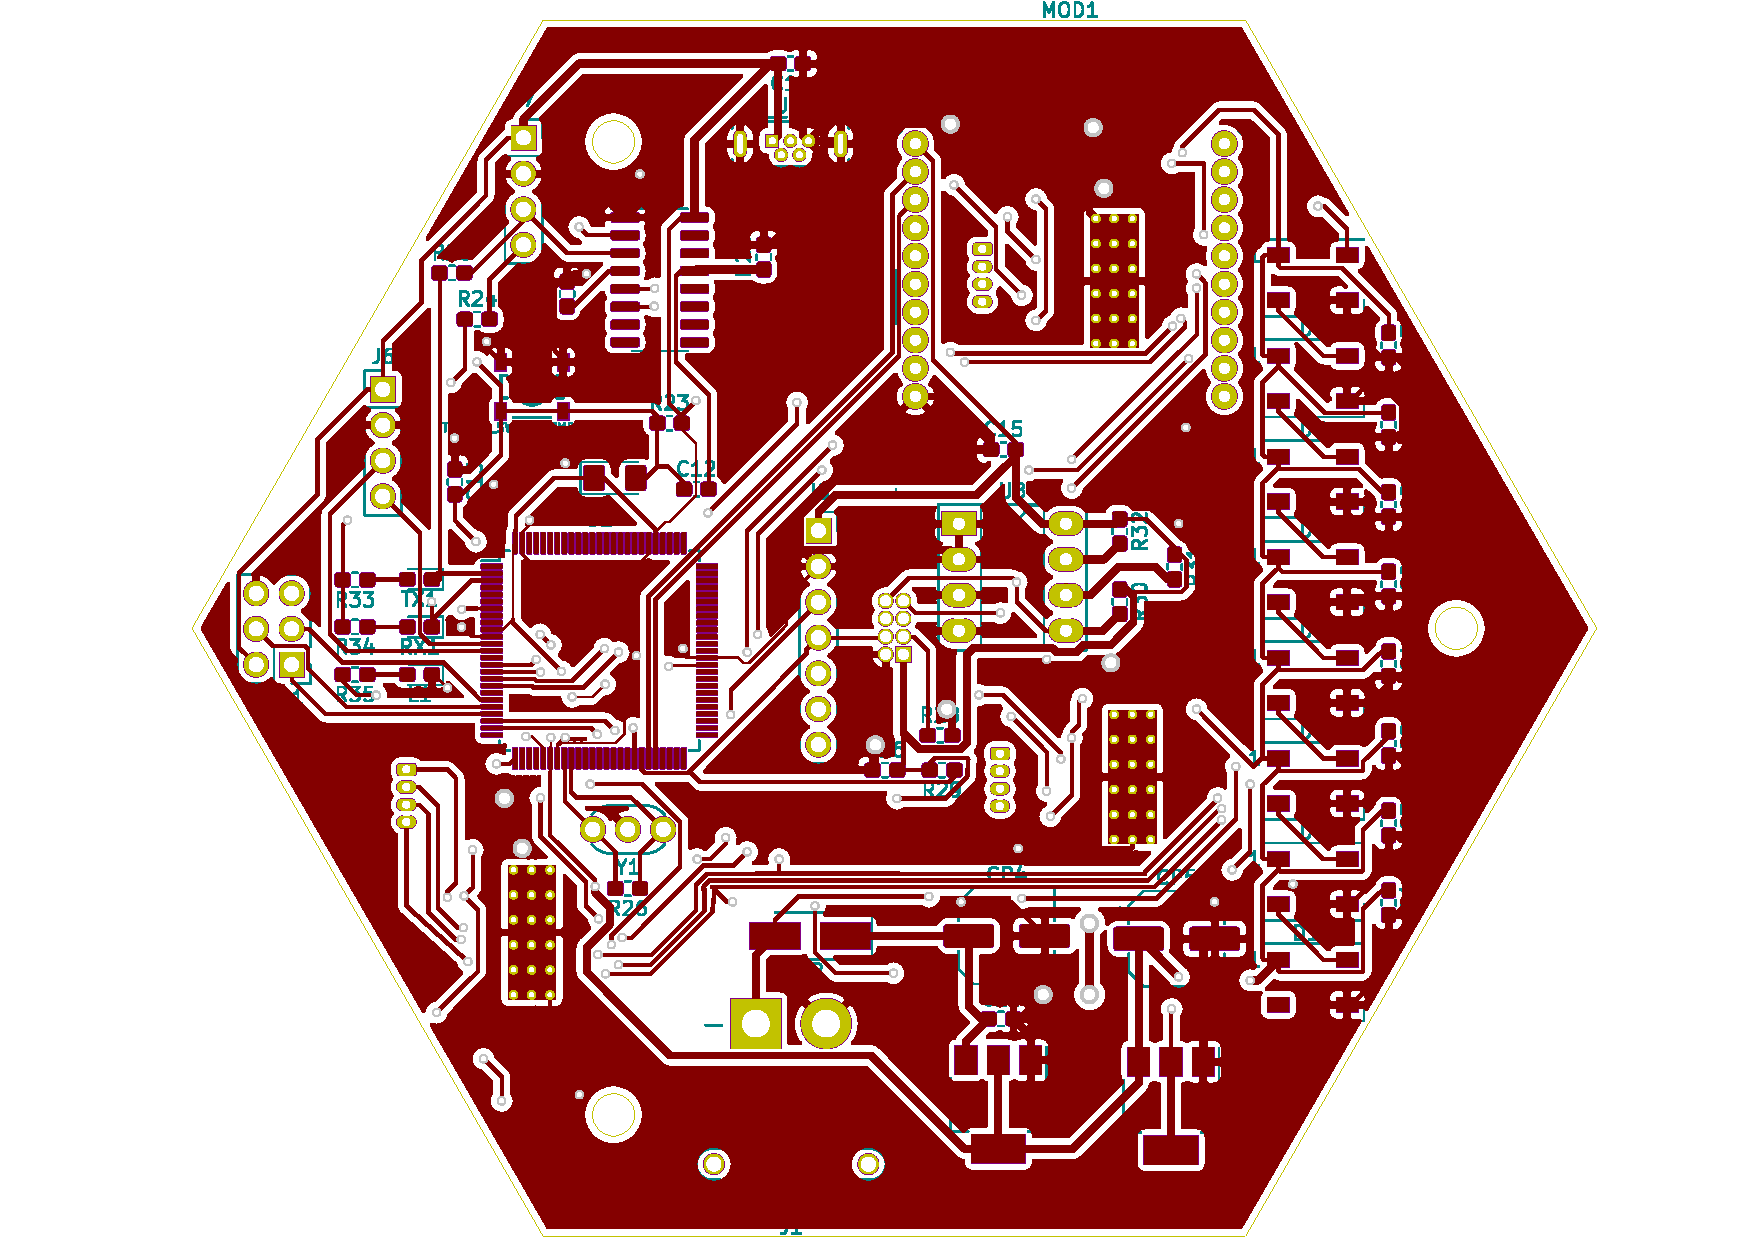
\includegraphics[width=\columnwidth]{CircuitPCB-F.pdf}
    \caption{PCB正面}
    \label{fig:CircuitPCB-F}
\end{figure}

\begin{figure}[htbp]
    \centering
    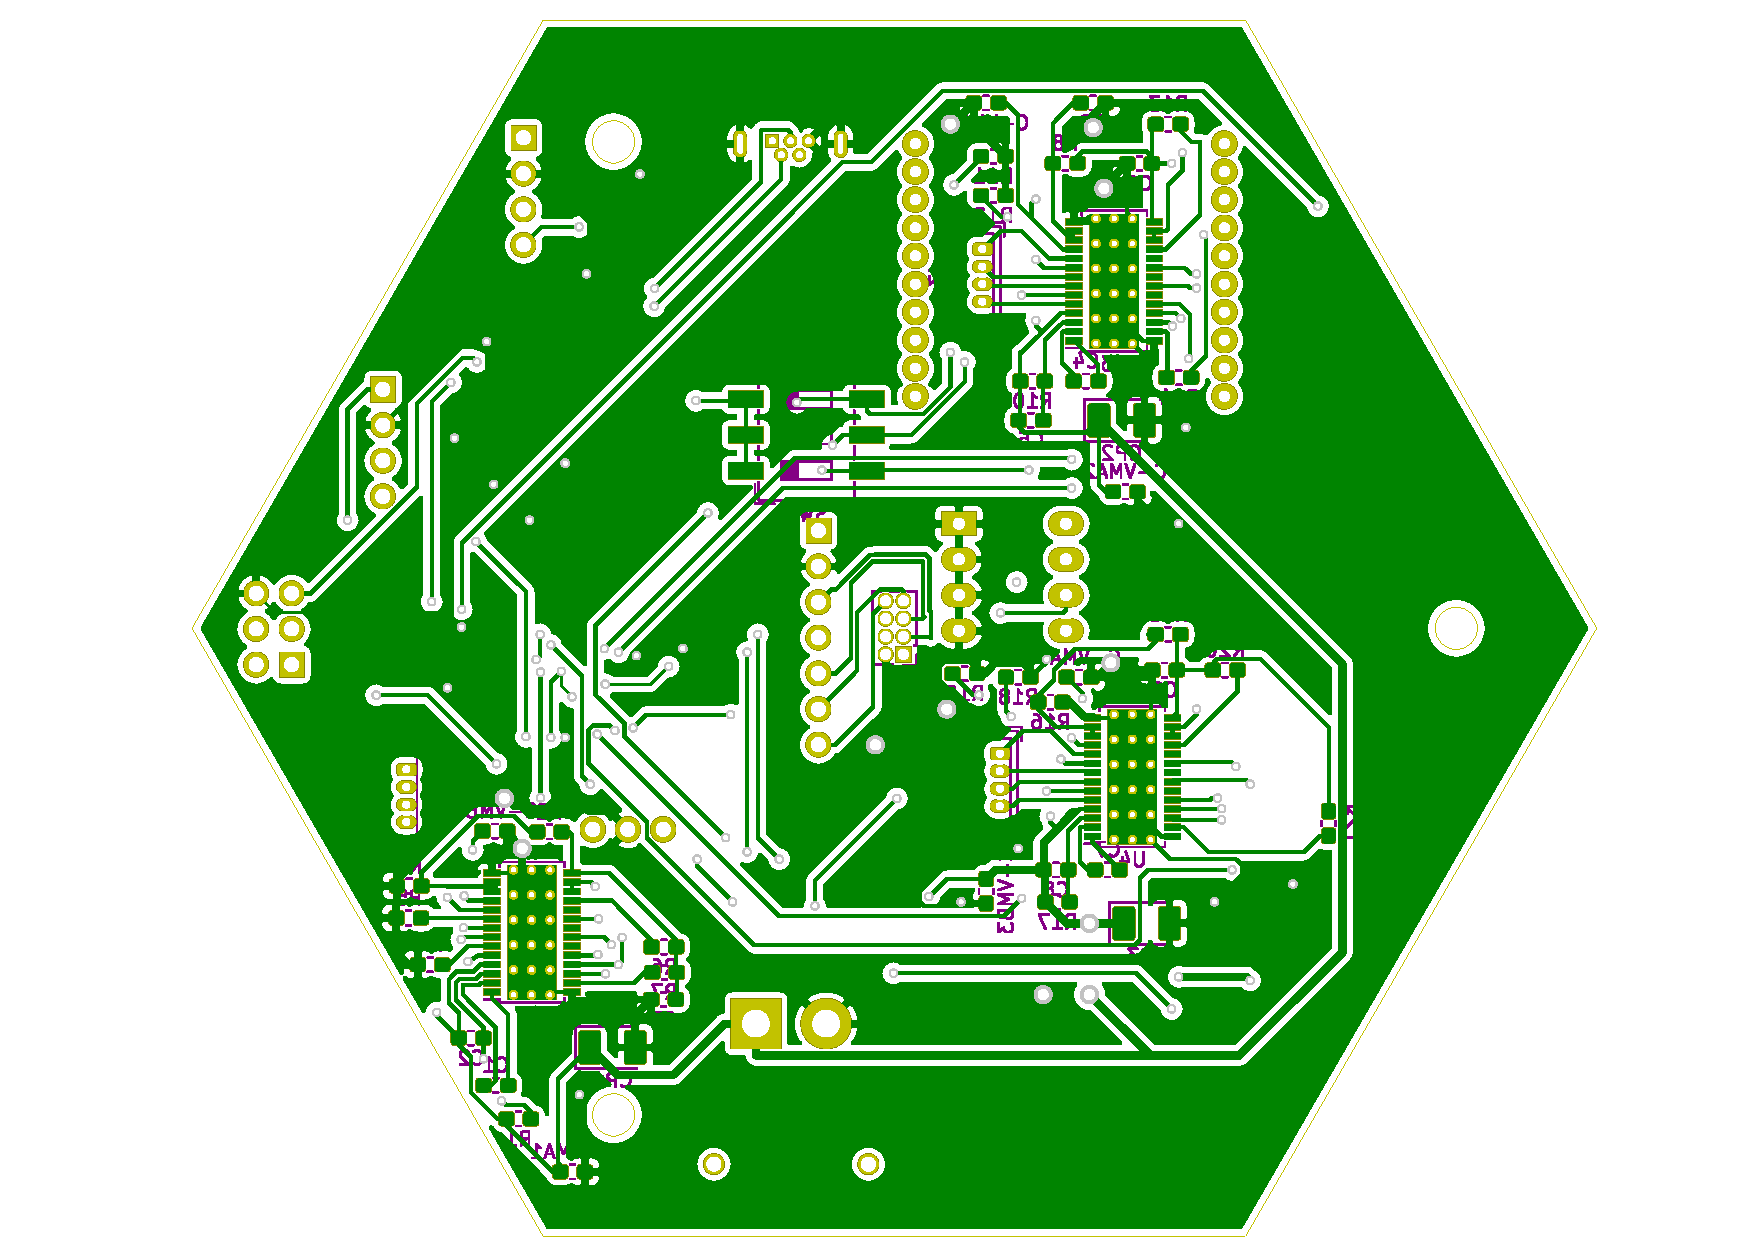
\includegraphics[width=\columnwidth]{CircuitPCB-B.pdf}
    \caption{PCB背面}
    \label{fig:CircuitPCB-B}
\end{figure}

\section{三维渲染图}

使用光线追踪技术对PCB模型进行渲染得到正反面的渲染图如图~\ref{fig:Circuit-Render}、~\ref{fig:Circuit-Render-2}、~\ref{fig:Circuit-Render-3}。

\begin{figure}[htbp]
    \centering
    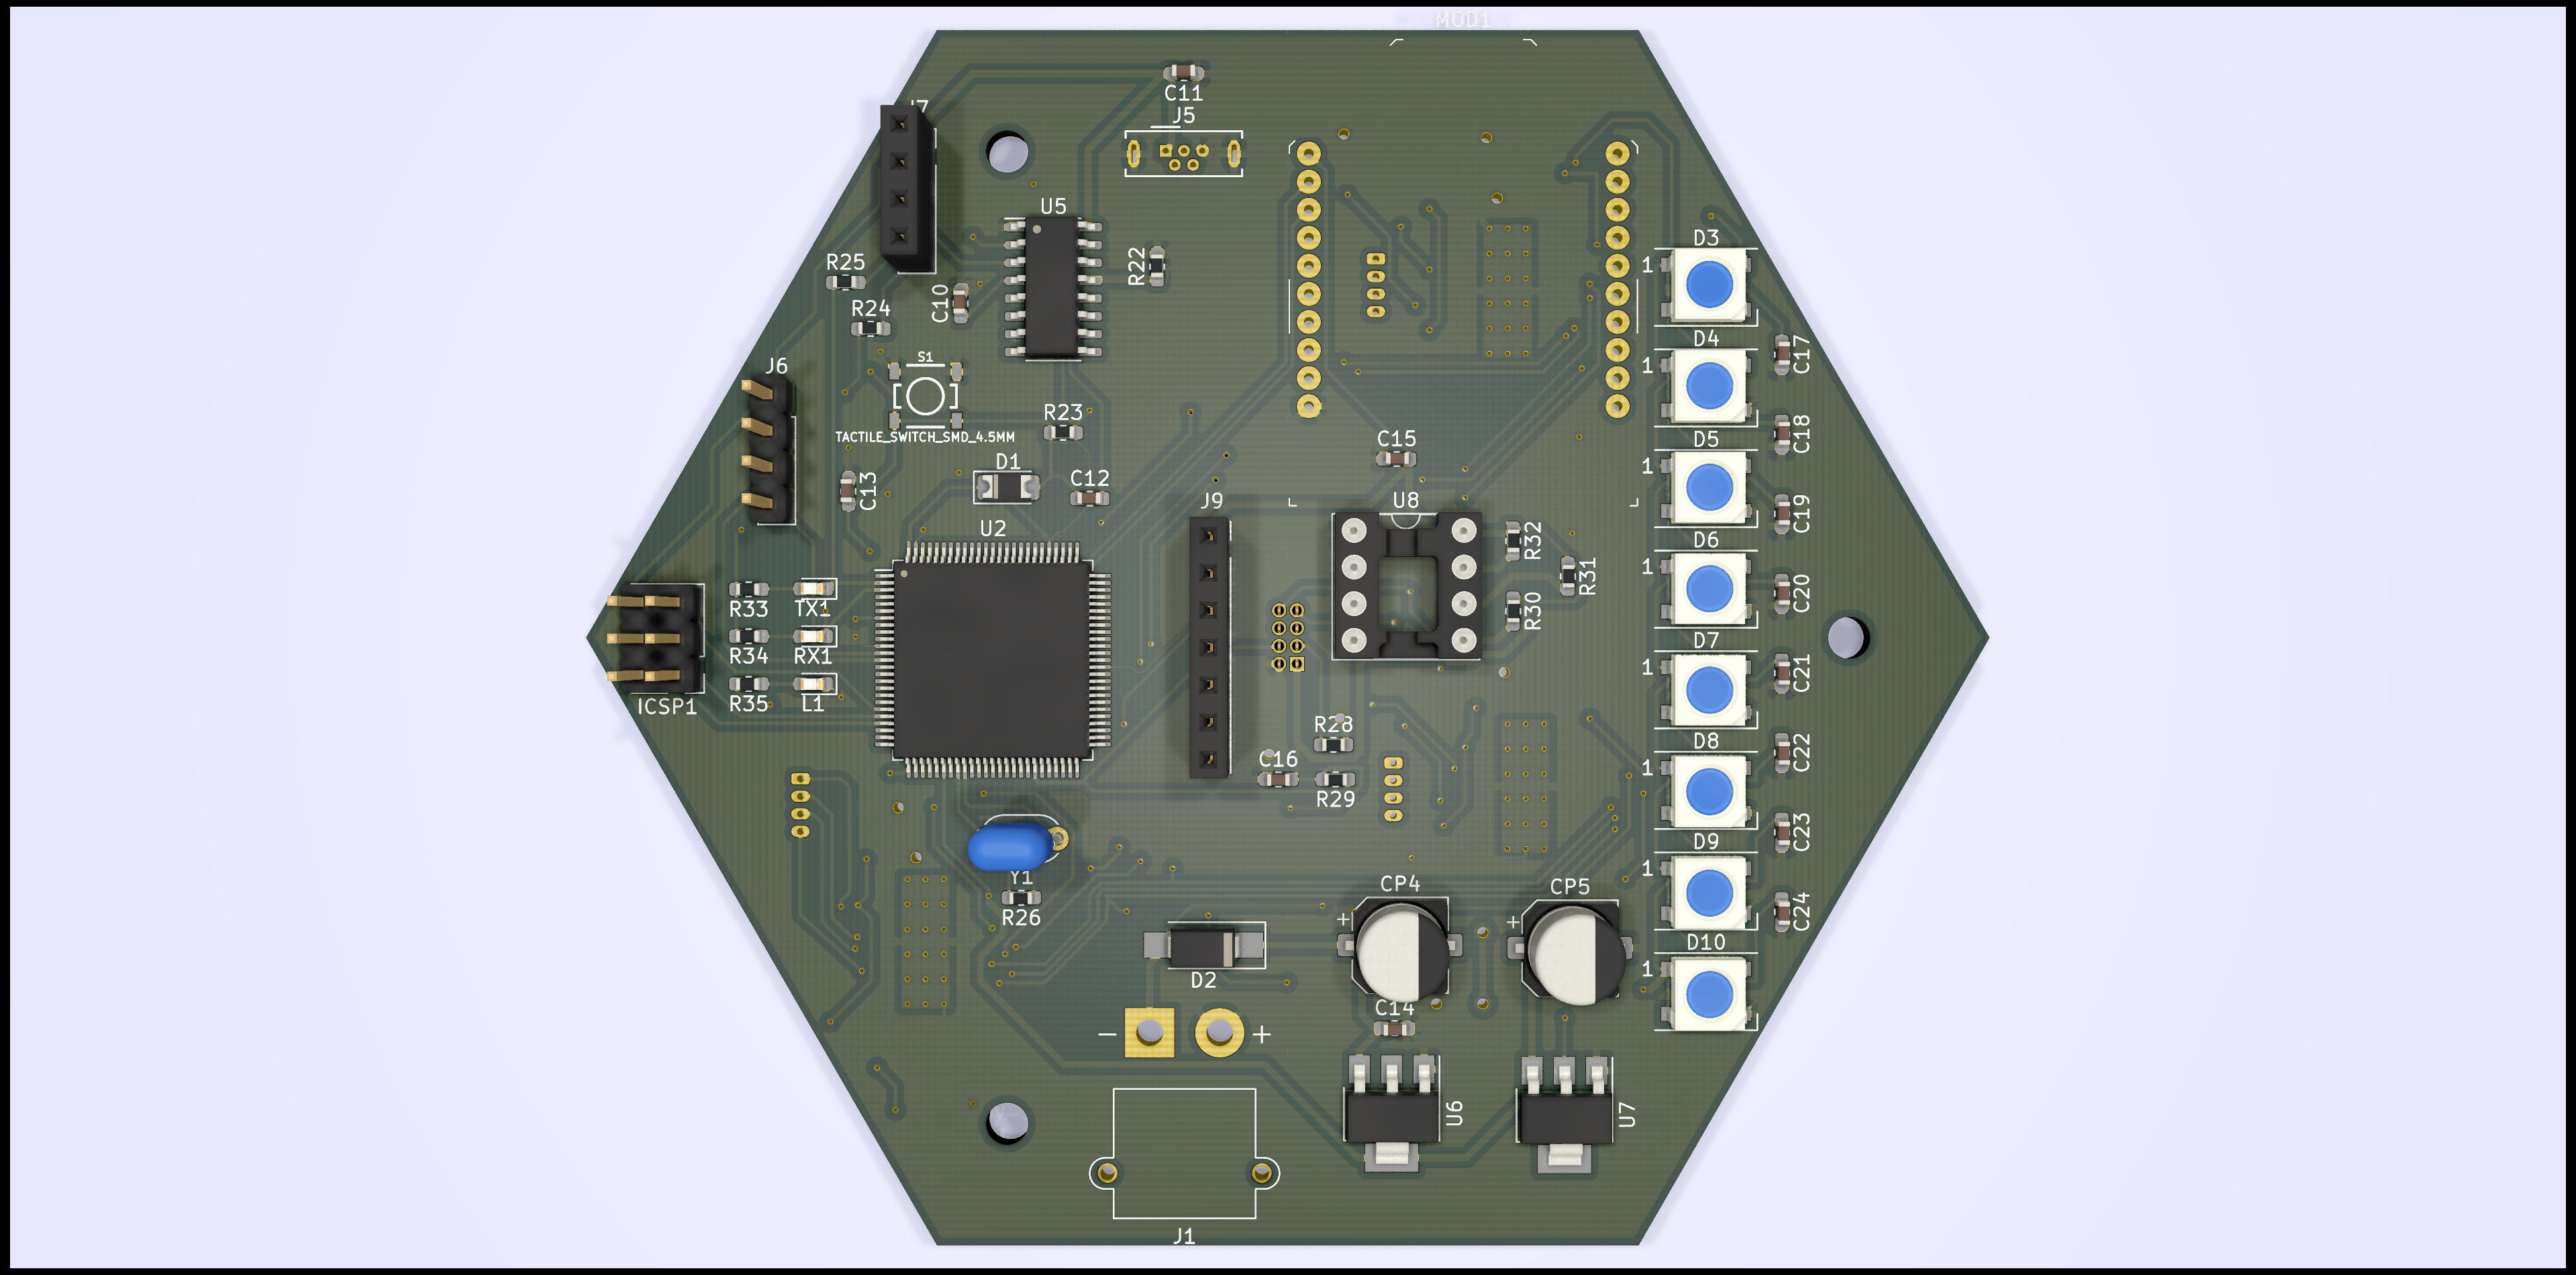
\includegraphics[width=\columnwidth]{Circuit.png}
    \caption{正面渲染图}
    \label{fig:Circuit-Render}
\end{figure}

\begin{figure}[htbp]
    \centering
    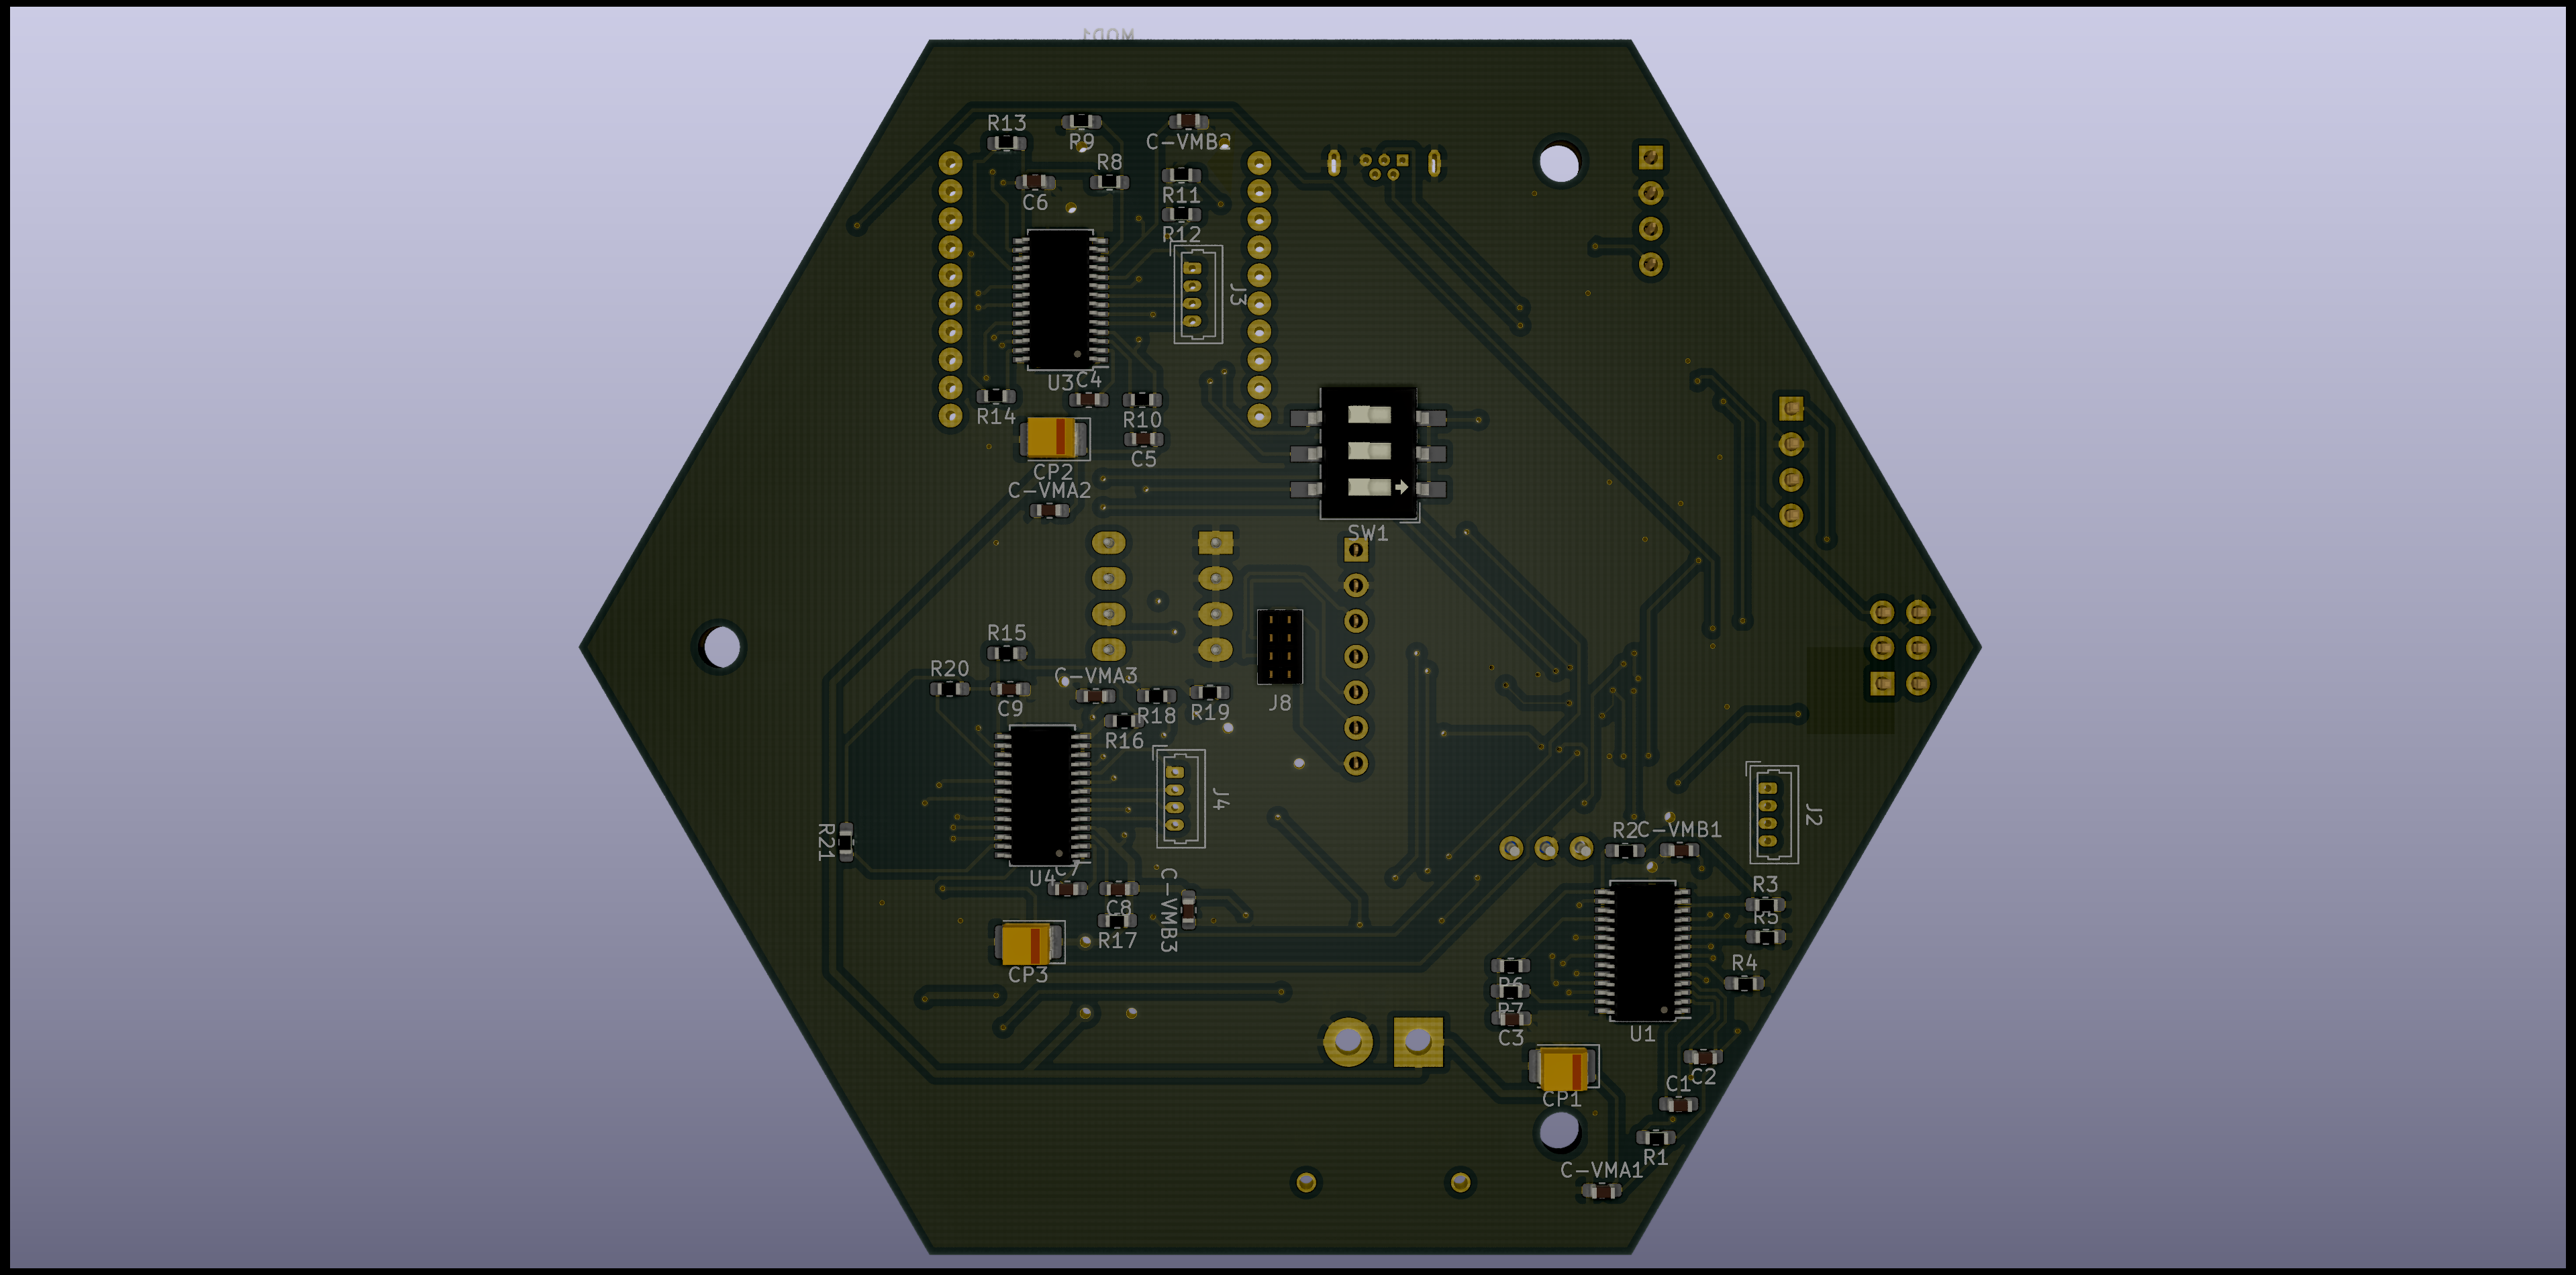
\includegraphics[width=\columnwidth]{Circuit-2.png}
    \caption{反面渲染图}
    \label{fig:Circuit-Render-2}
\end{figure}

\begin{figure}[htbp]
    \centering
    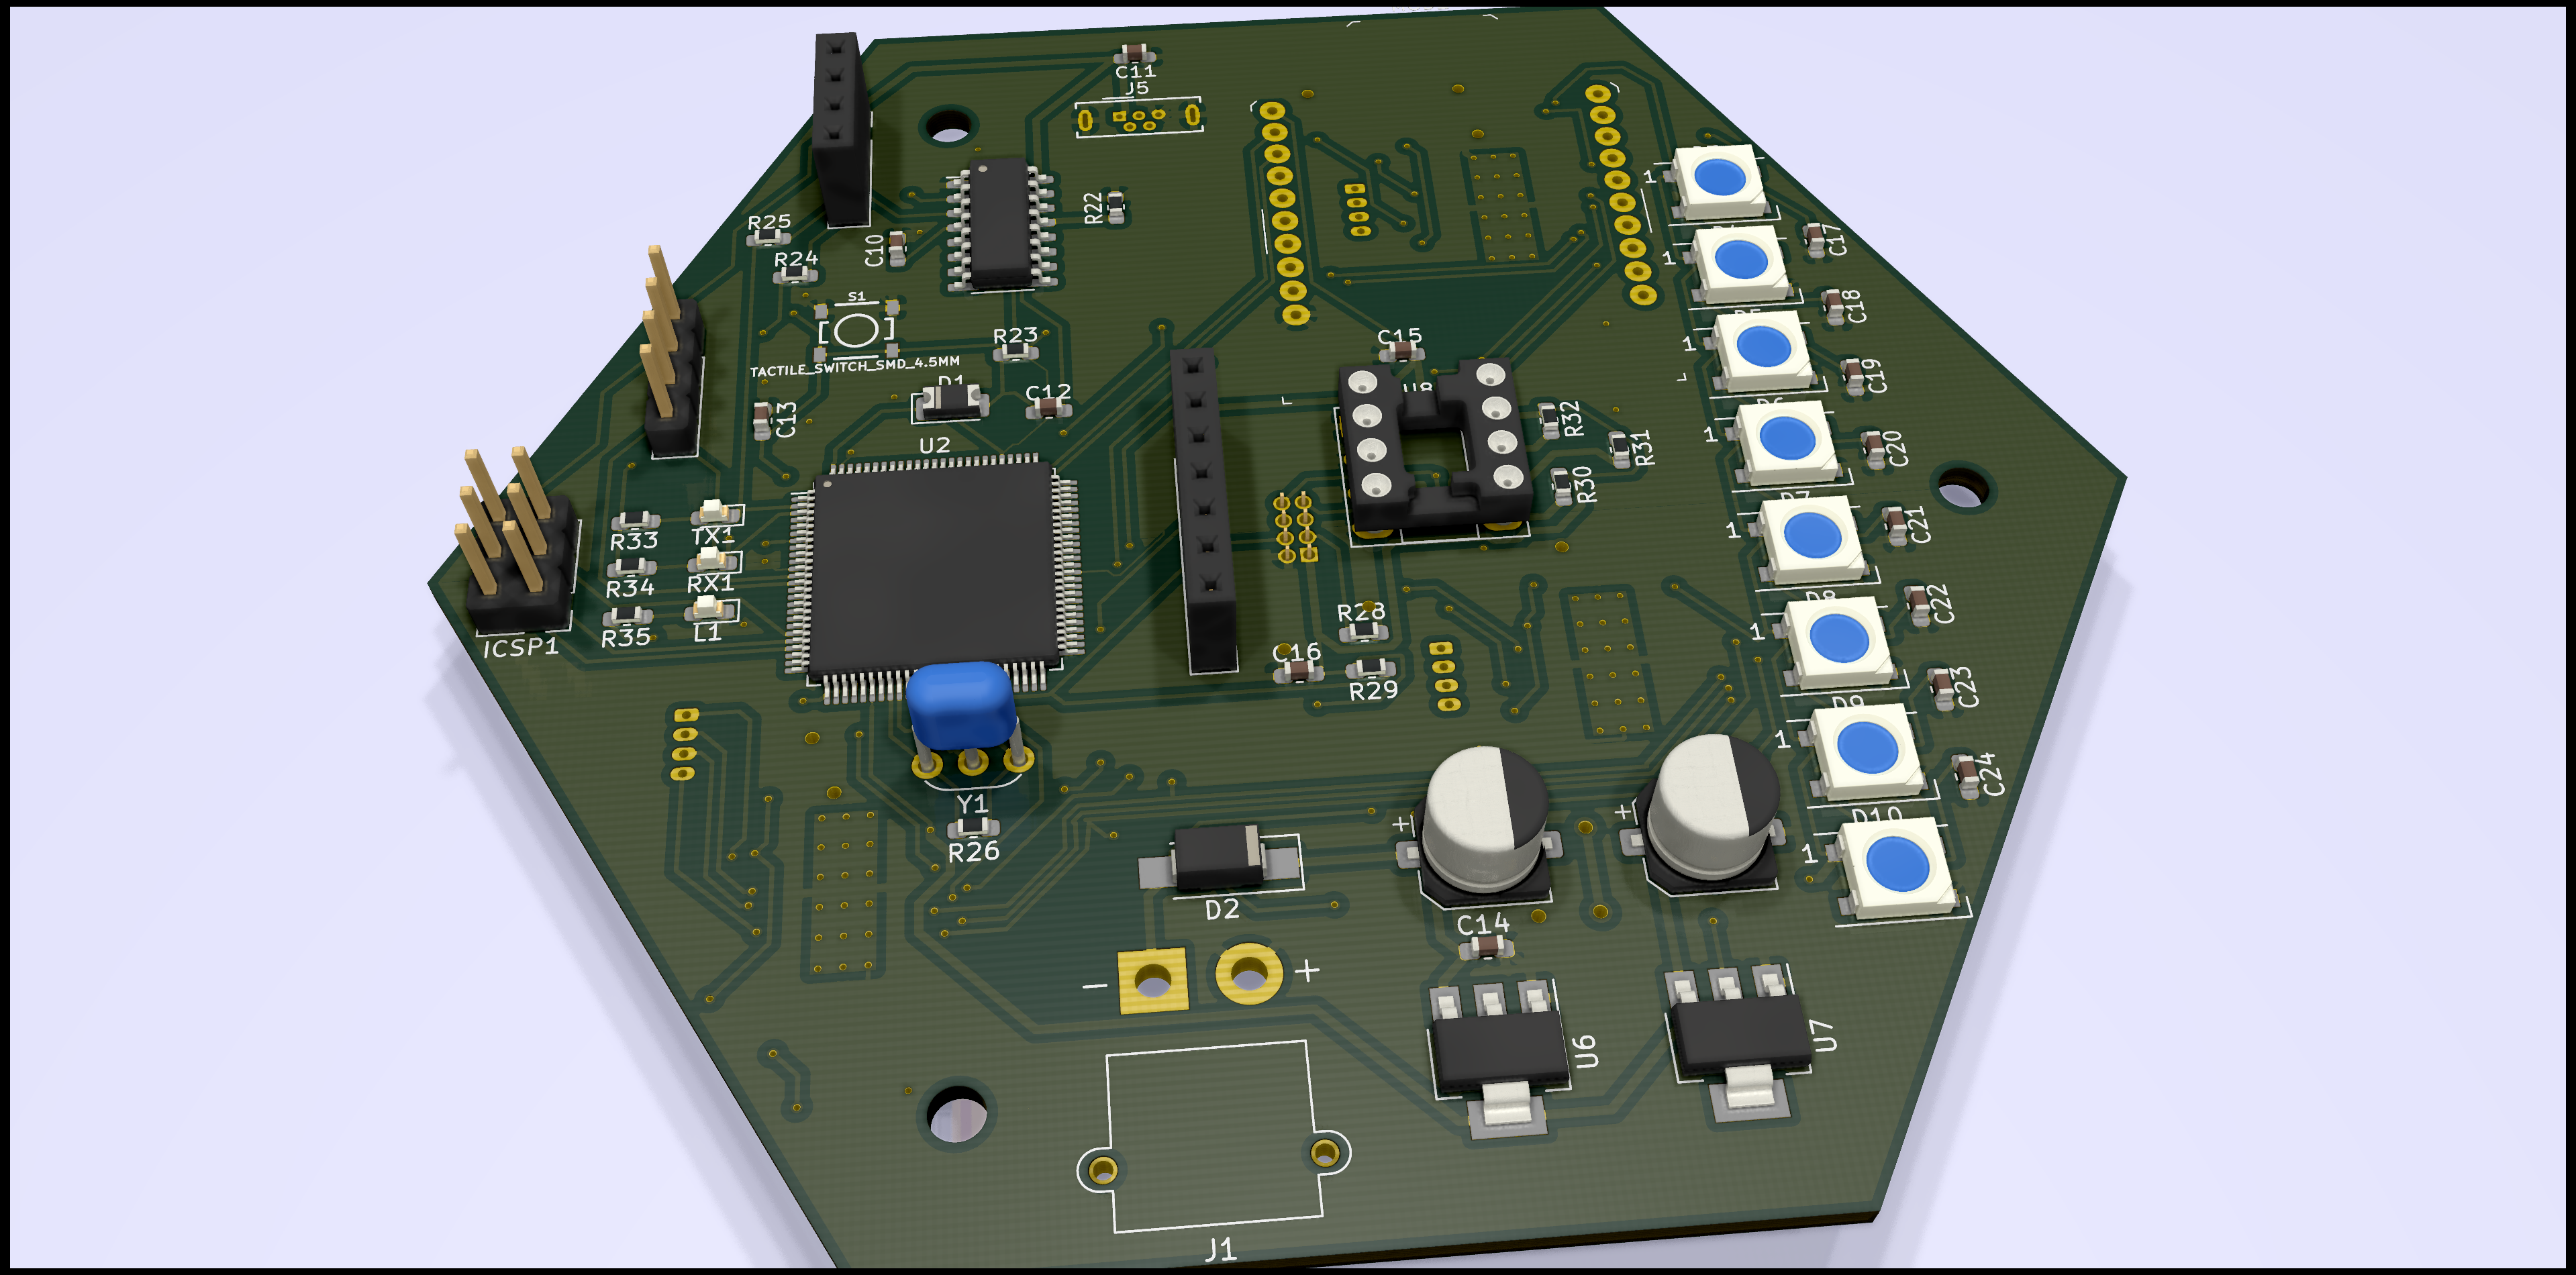
\includegraphics[width=\columnwidth]{Circuit-3.png}
    \caption{侧视渲染图}
    \label{fig:Circuit-Render-3}
\end{figure}

\section{导出Gerber交付打样}

在File-Plot-Gerber中选中需要的层,压缩上传。

\section{焊接}

使用InteractiveHtmlBom\footnote{\url{https://github.com/openscopeproject/InteractiveHtmlBom}}(Interactive HTML BOM plugin for KiCad)工具导出了HTML BOM方便焊接时对照BOM,如图~\ref{fig:InteractiveHtmlBom}。

\begin{figure}[htbp]
    \centering
    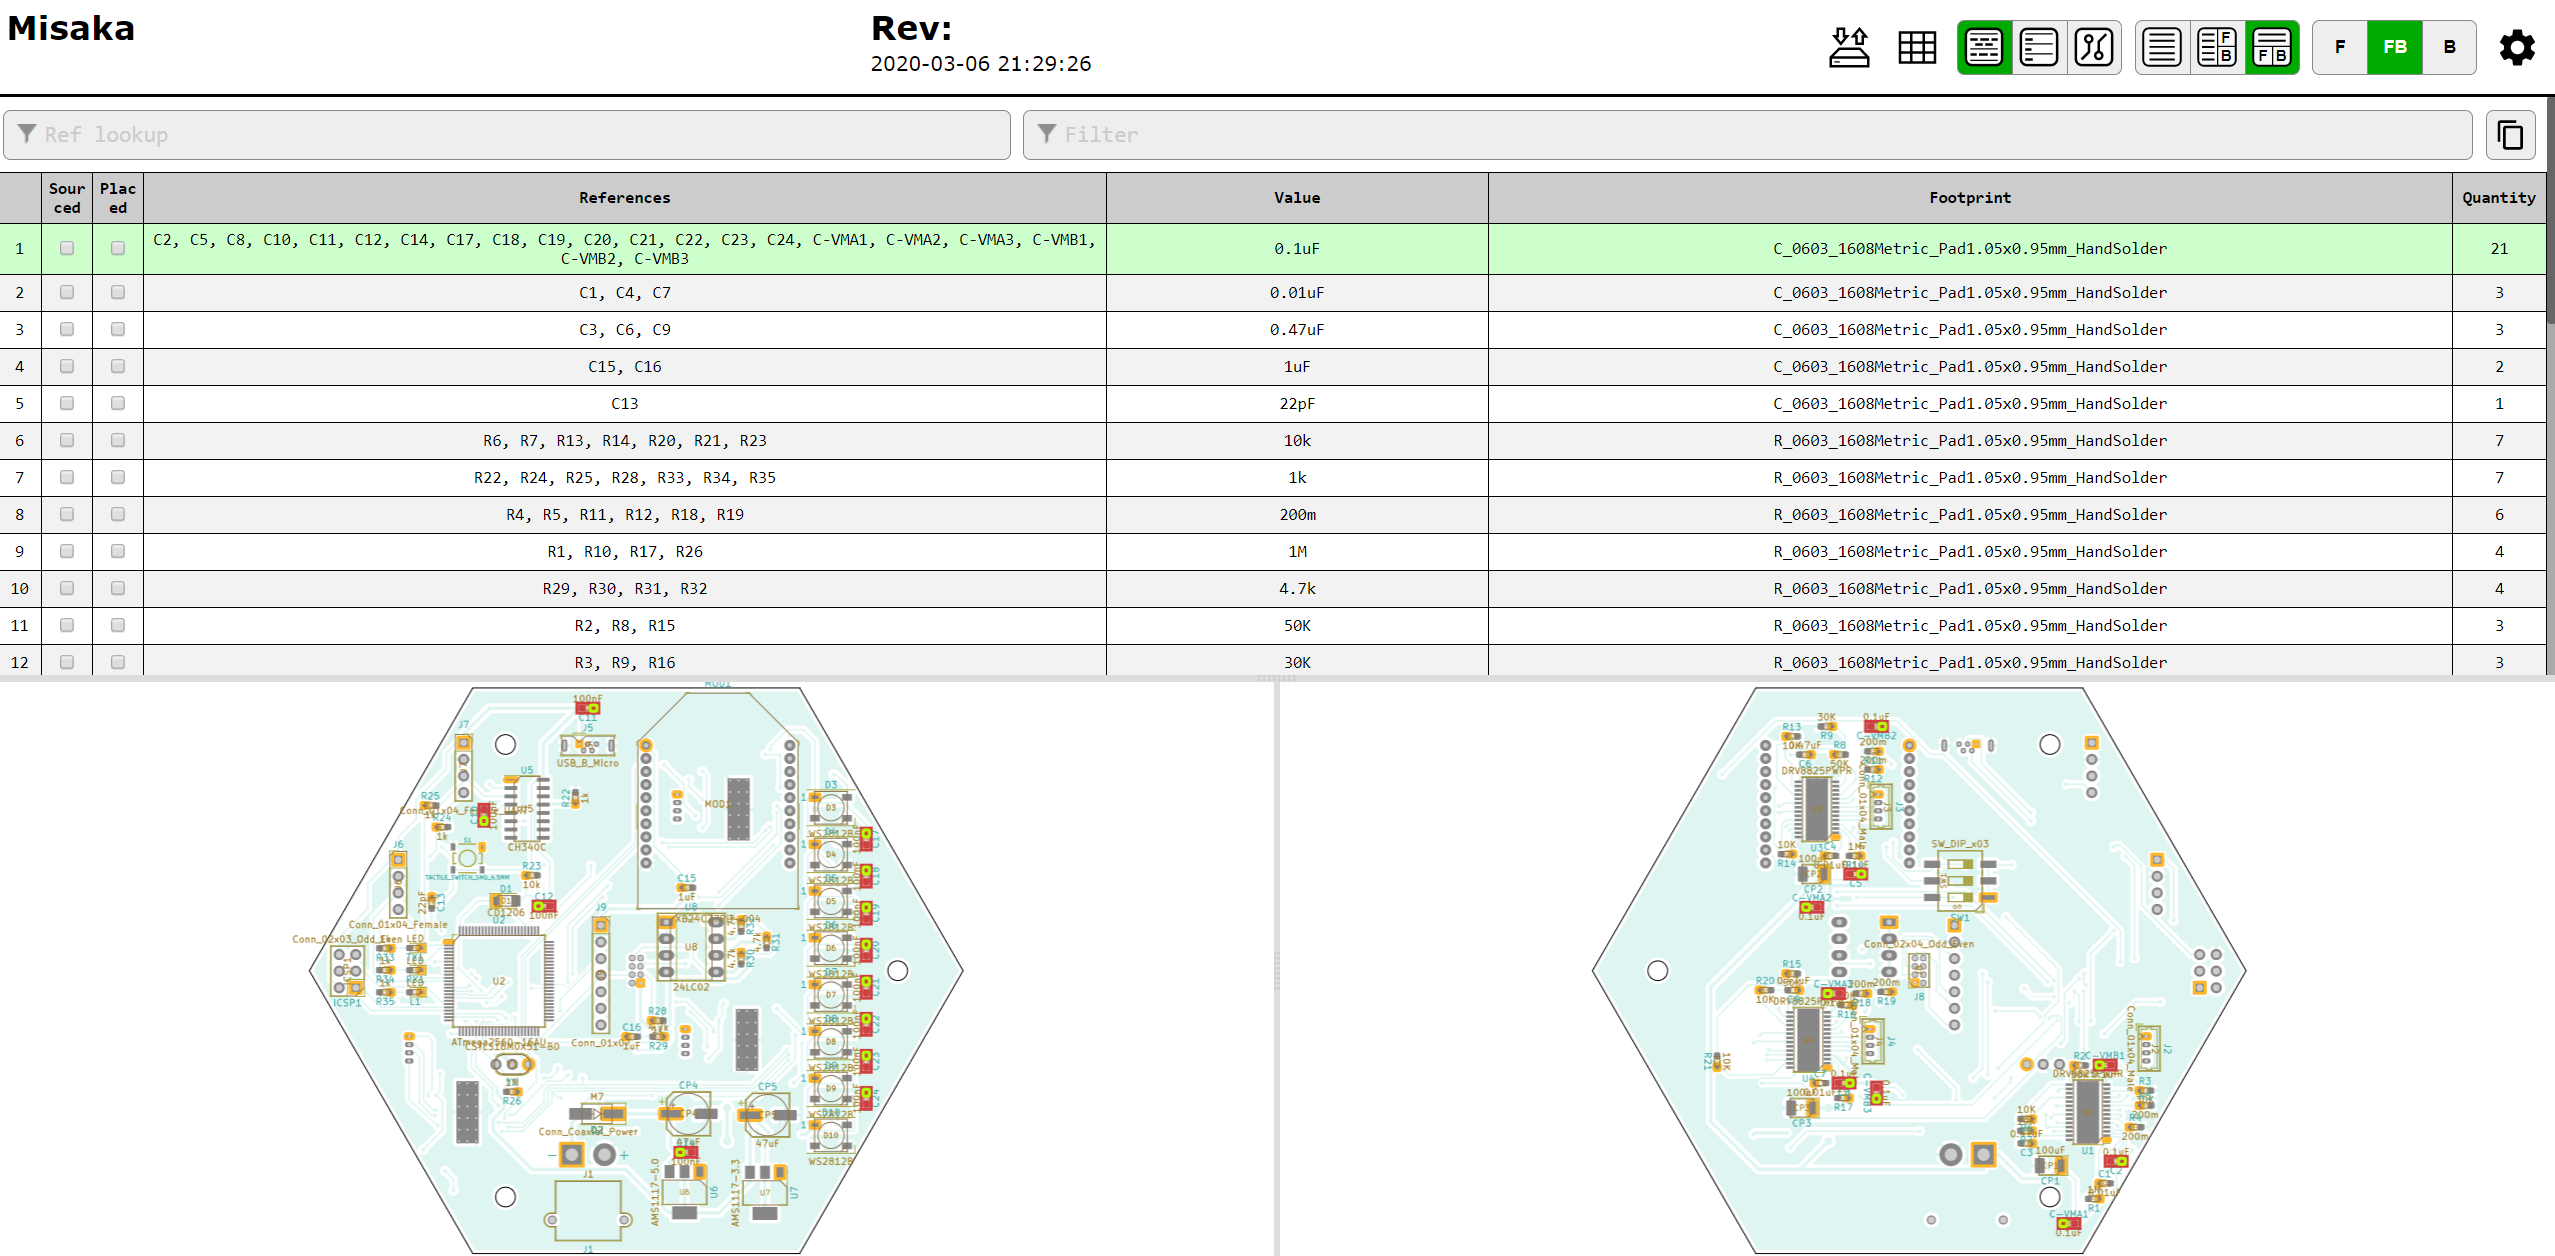
\includegraphics[width=\columnwidth]{InteractiveHtmlBom.png}
    \caption{InteractiveHtmlBom}
    \label{fig:InteractiveHtmlBom}
\end{figure}

由于AT Mega的100A, 100-lead, 14 x 14 mm Body Size, 1.0 mm Body Thickness, 0.5 mm Lead Pitch, Thin Profile Plastic Quad Flat Package (TQFP)封装较难手焊,于是定制了相应的激光钢网,涂锡膏(solder paste)之后摆上元件,并使用相应的恒温锡炉加热融化锡膏,这里使用的是138度熔点的千住锡浆,锡炉温度设定在180摄氏度。如图~\ref{fig:ApplySolderPaste}。

\begin{figure}[htbp]
    \centering
    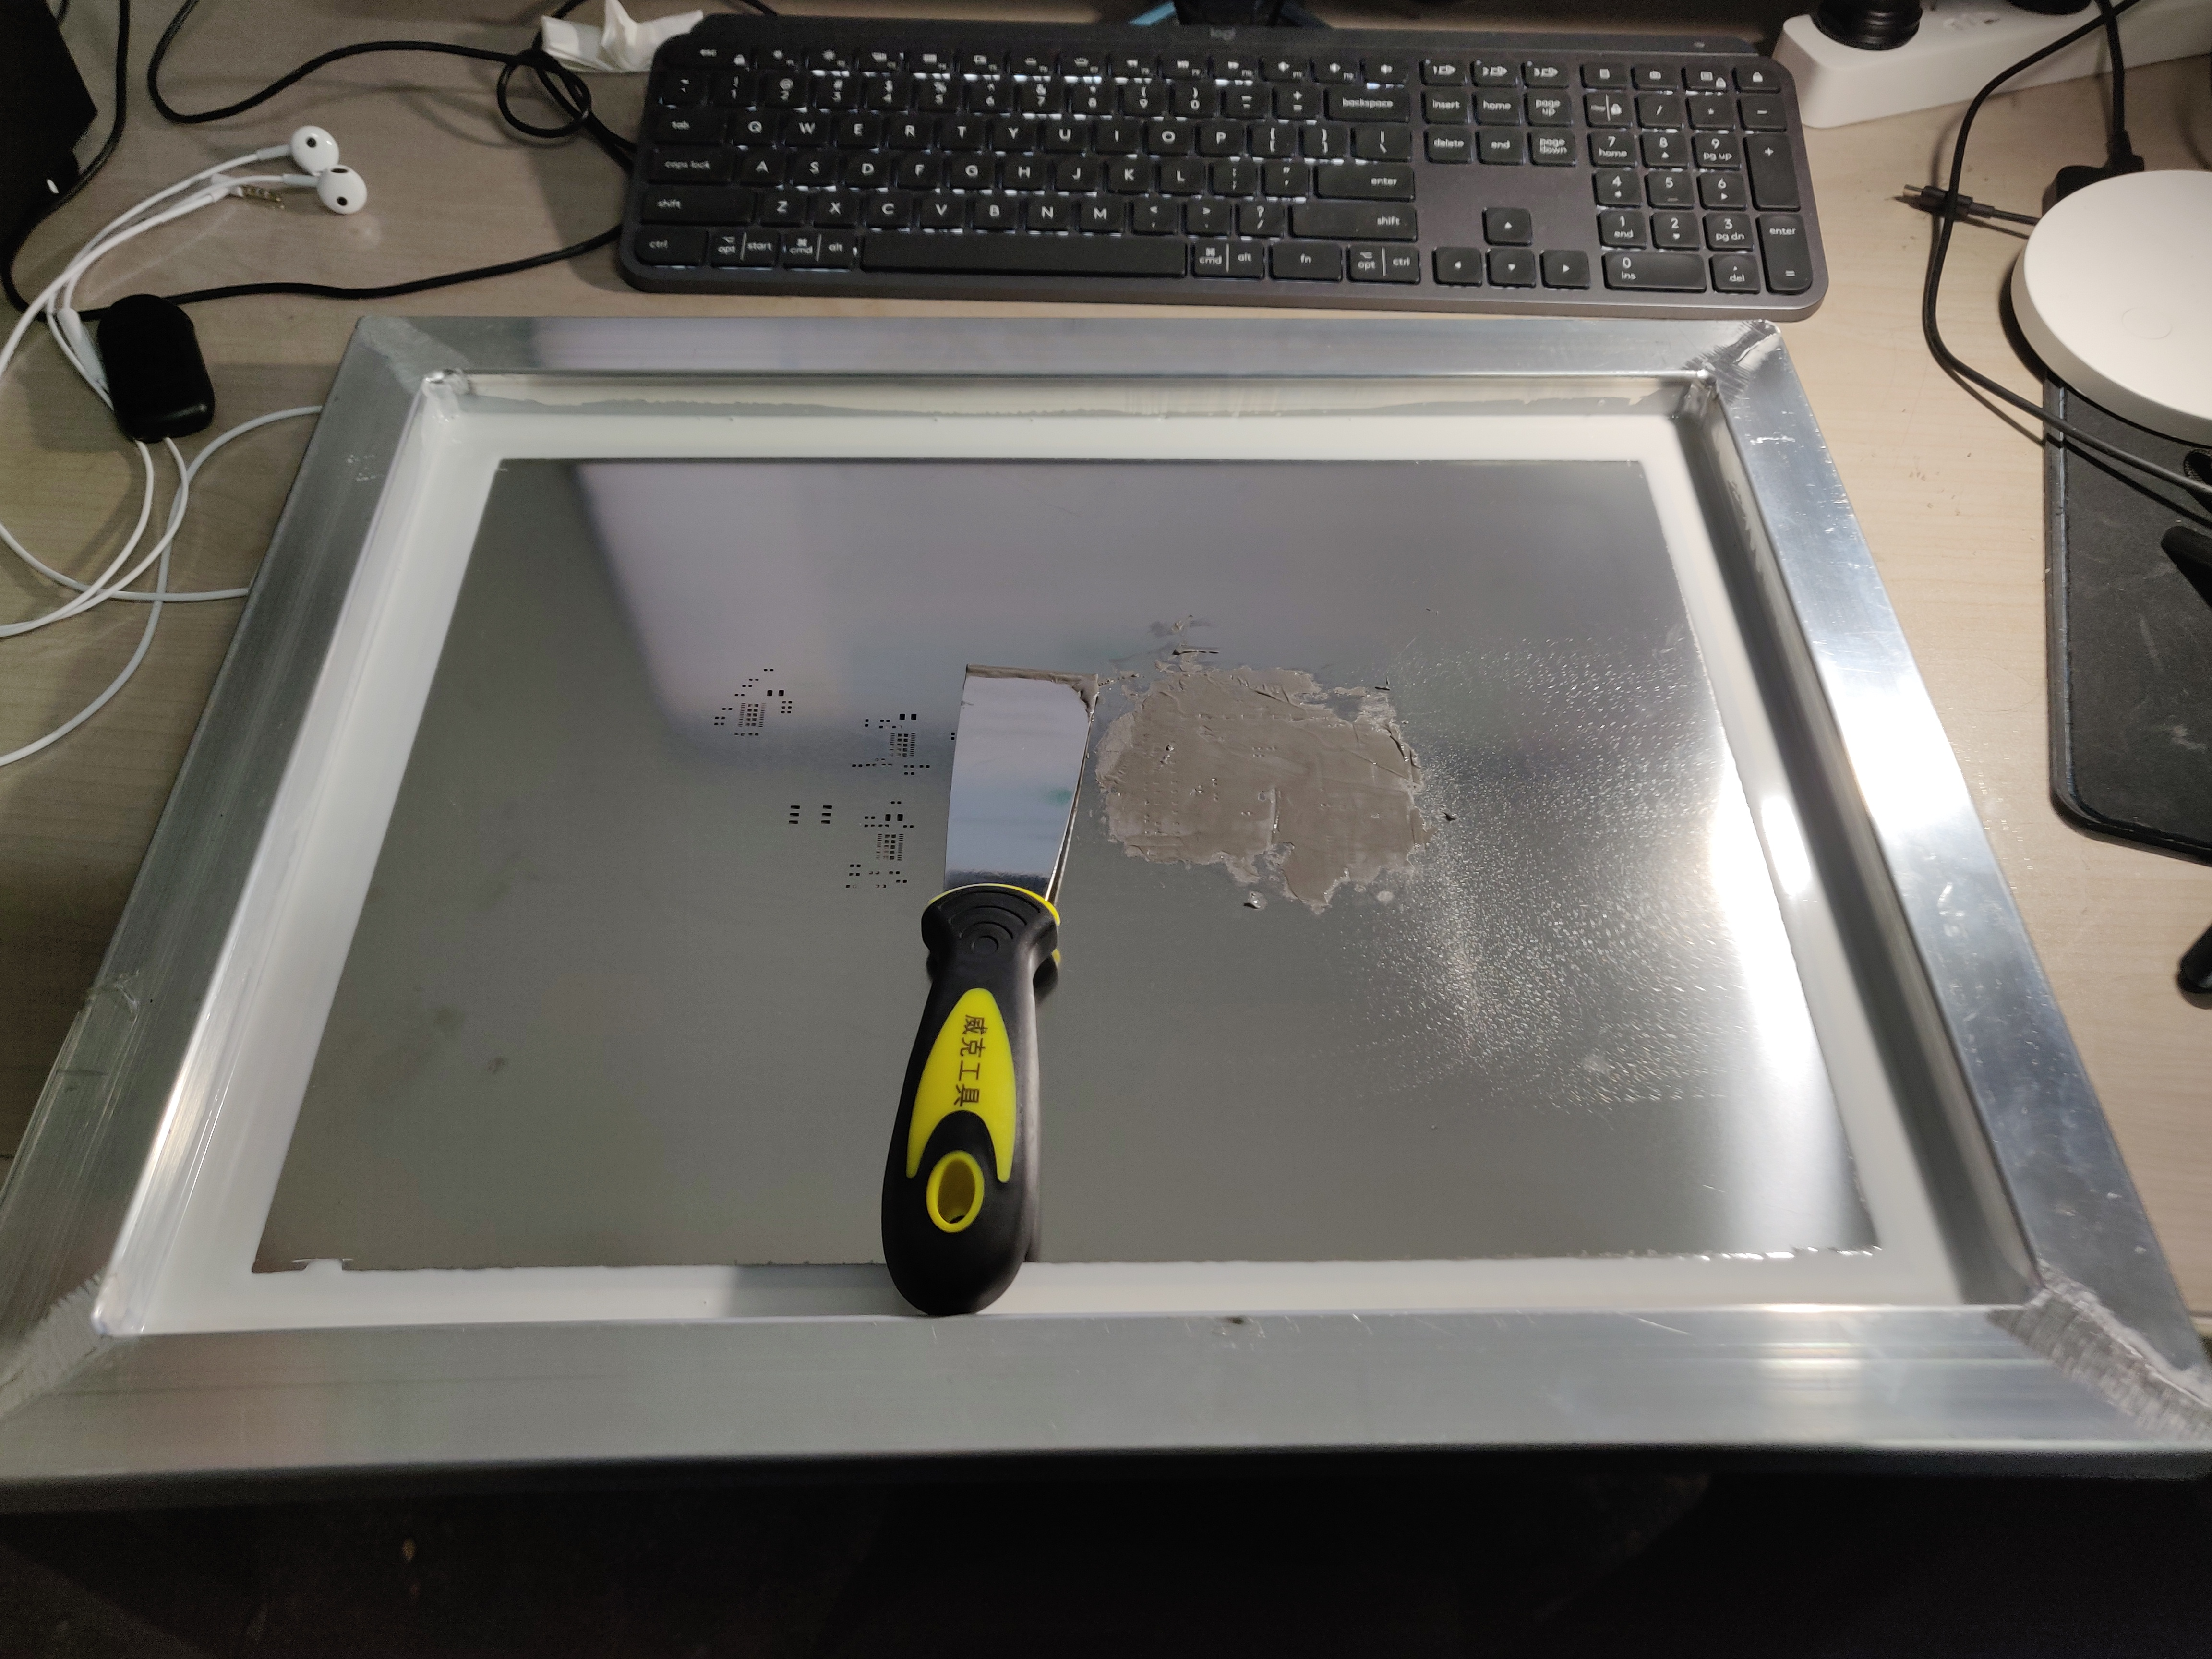
\includegraphics[width=\columnwidth]{PCBv2ApplySolderPaste.jpg}
    \caption{激光钢网涂锡膏}
    \label{fig:ApplySolderPaste}
\end{figure}

\begin{figure}[htbp]
    \centering
    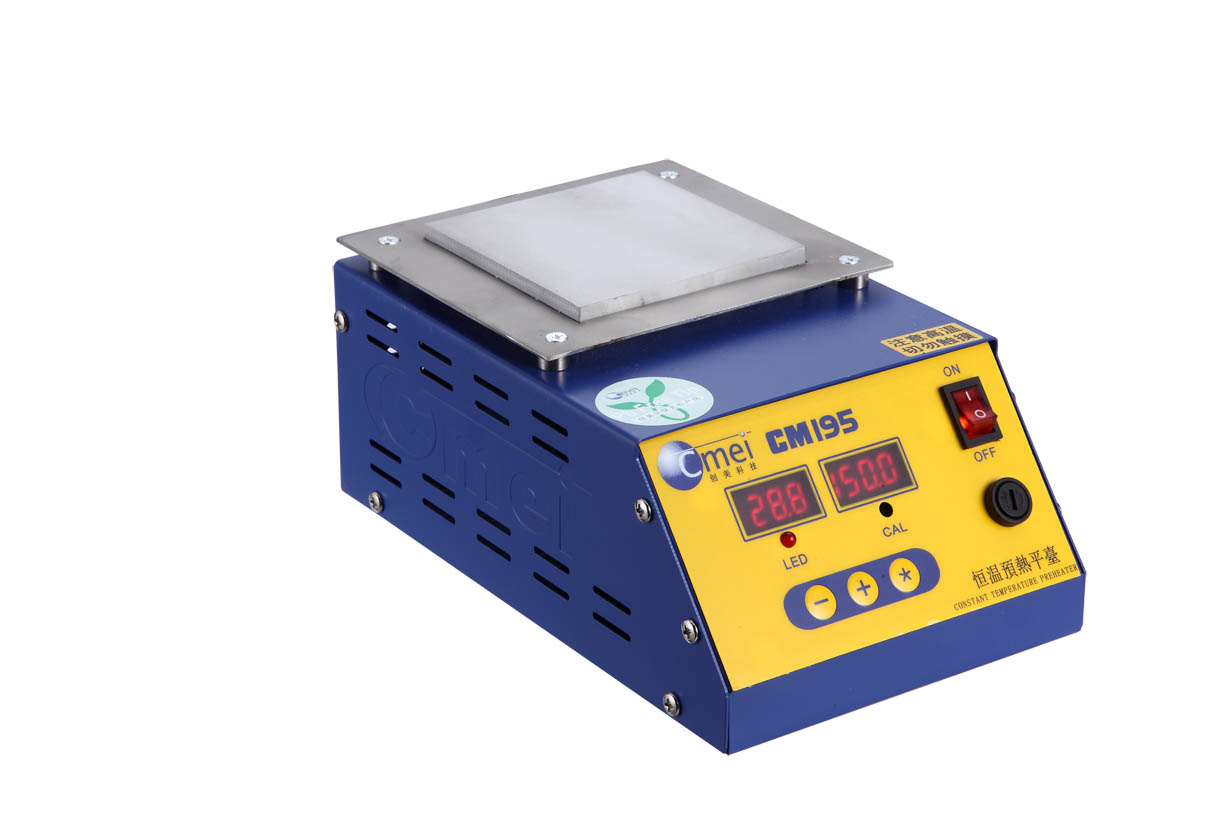
\includegraphics[width=\columnwidth]{SolderOven.jpg}
    \caption{恒温锡炉(无铅预热平台)}
    \label{fig:SolderOven}
\end{figure}


正面焊完效果如图~\ref{fig:PCBv2Soldring}。

\begin{figure}[htbp]
    \centering
    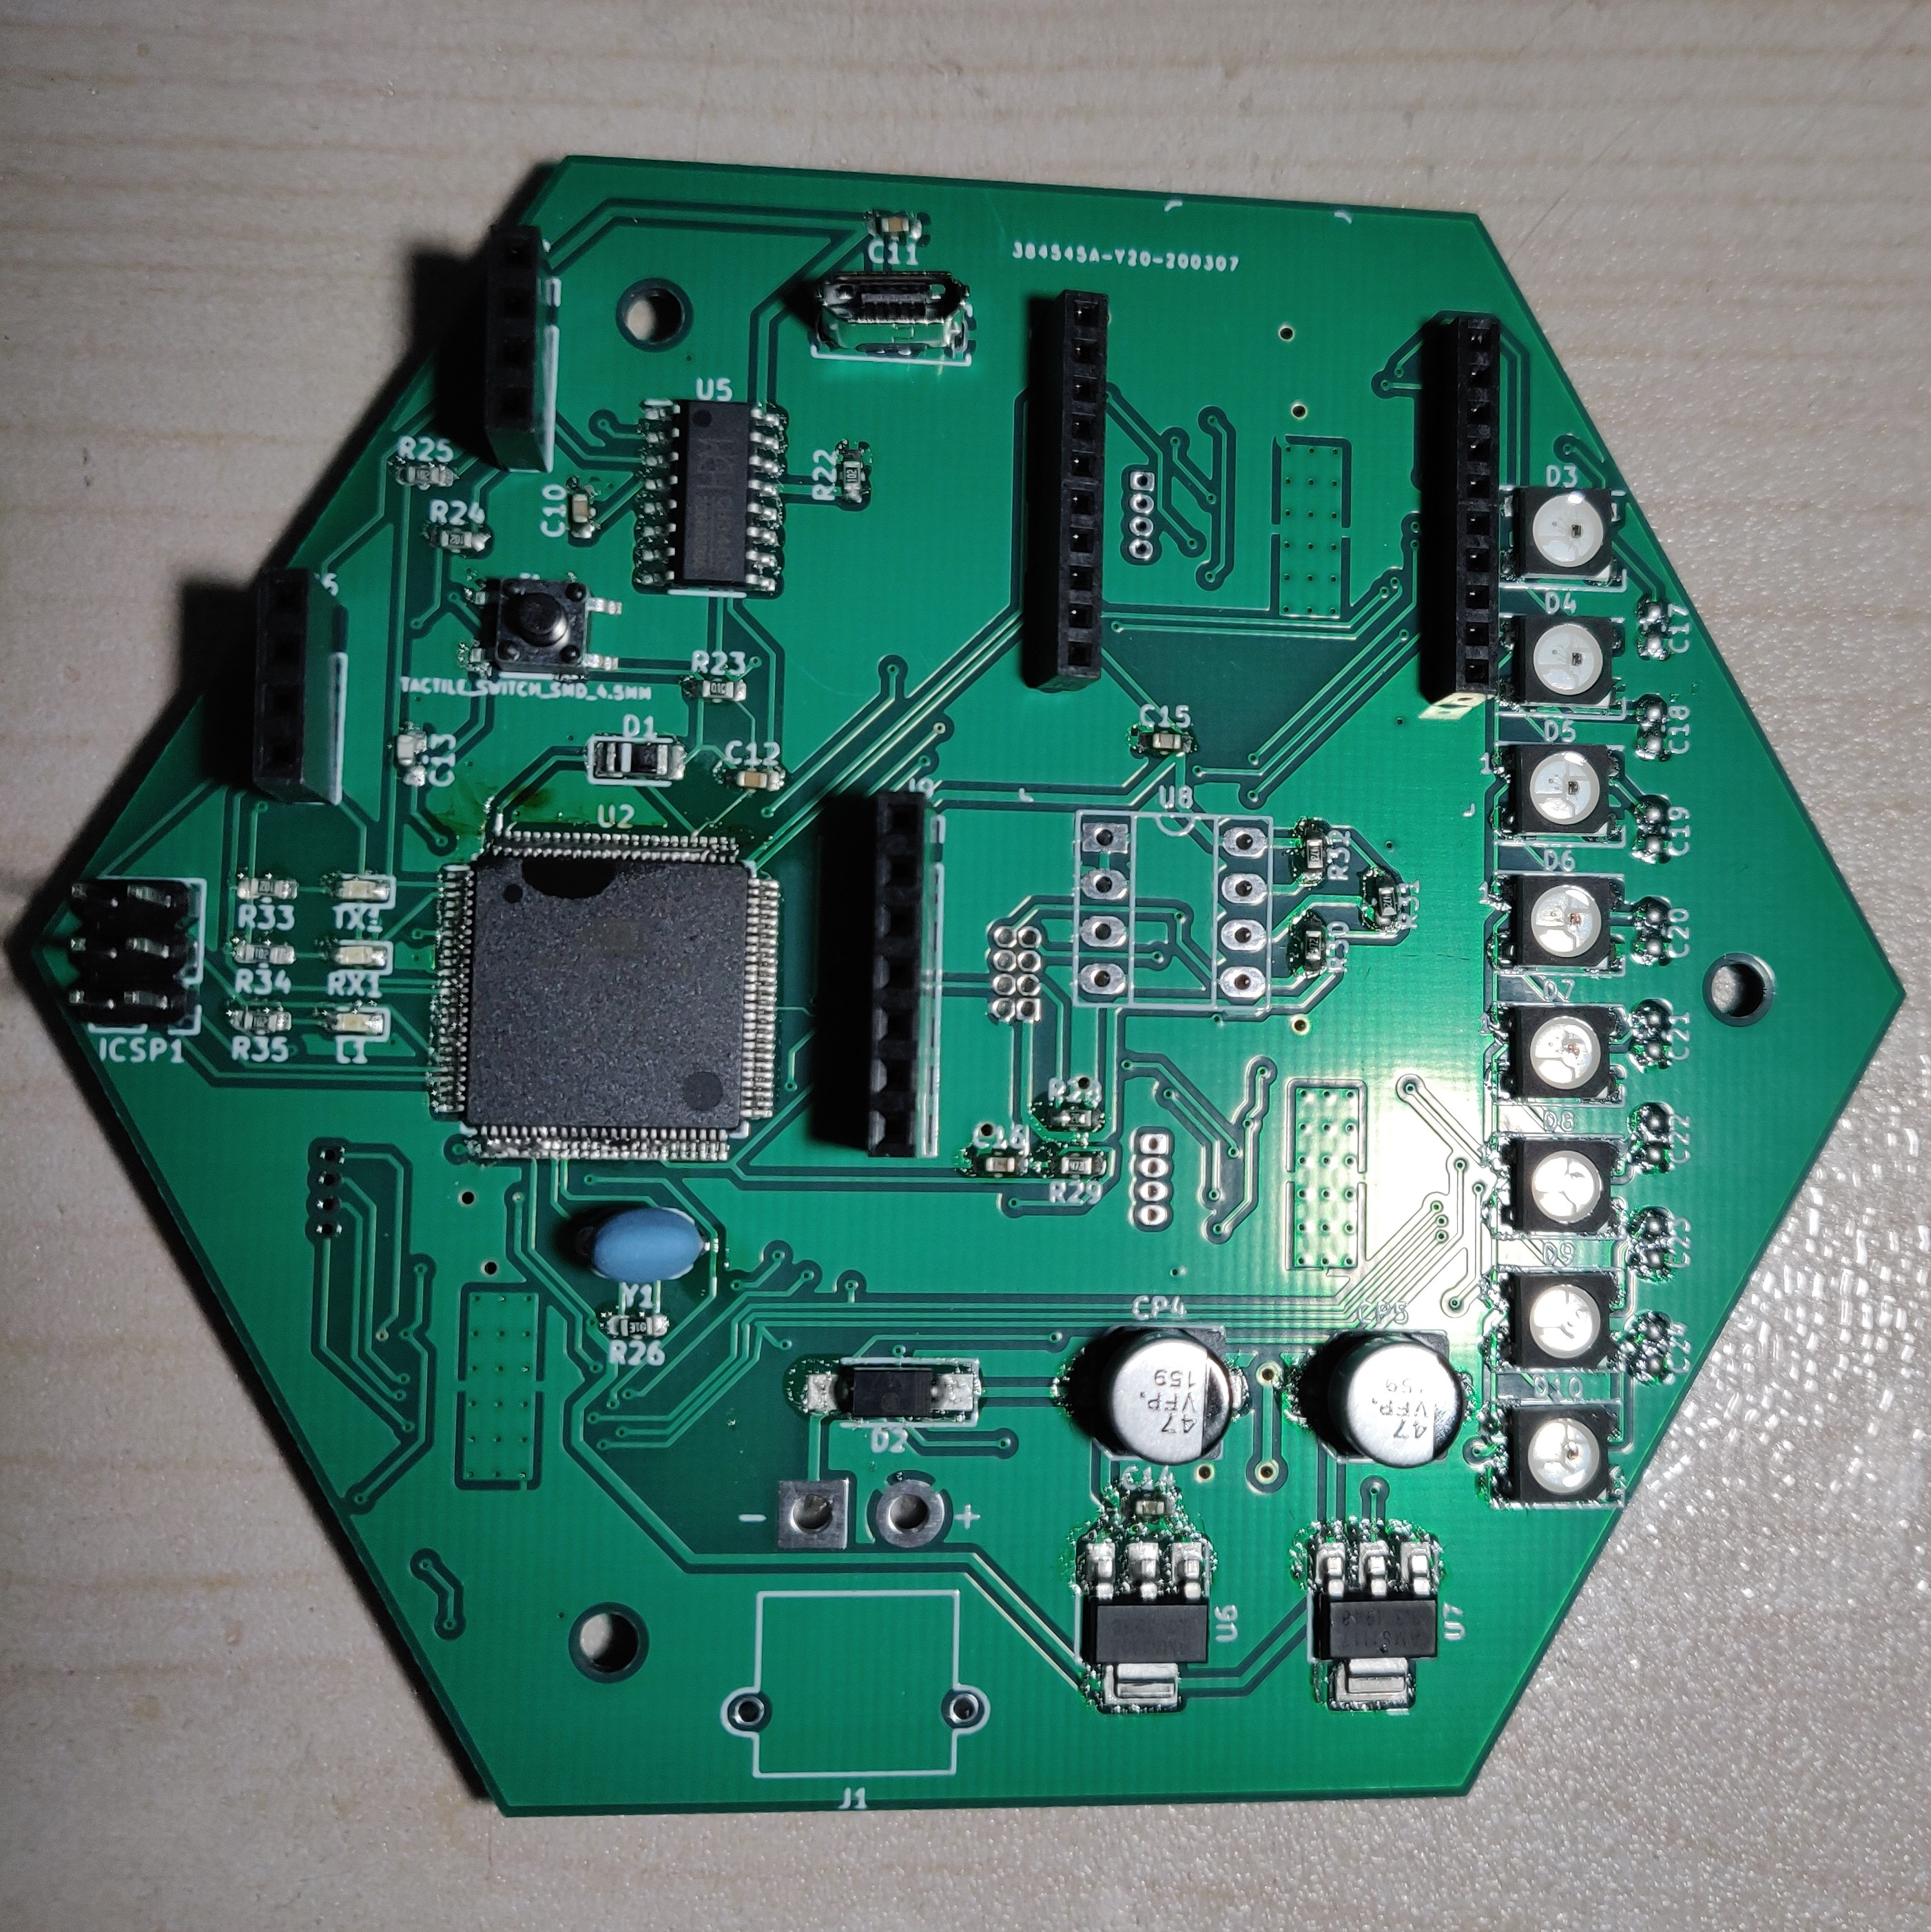
\includegraphics[width=\columnwidth]{PCBv2Soldring.jpg}
    \caption{正面焊完效果}
    \label{fig:PCBv2Soldring}
\end{figure}

使用Arduino as ISP烧写Blink和Floar LED String Test程序,测试部分功能正常。如图~\ref{fig:PCBv2ISP}和图~\ref{fig:PCBv2Test}。

\begin{figure}[htbp]
    \centering
    \includegraphics[width=\columnwidth]{PCBv2ISP.jpg}
    \caption{使用Arduino as ISP烧写}
    \label{fig:PCBv2ISP}
\end{figure}

\begin{figure}[htbp]
    \centering
    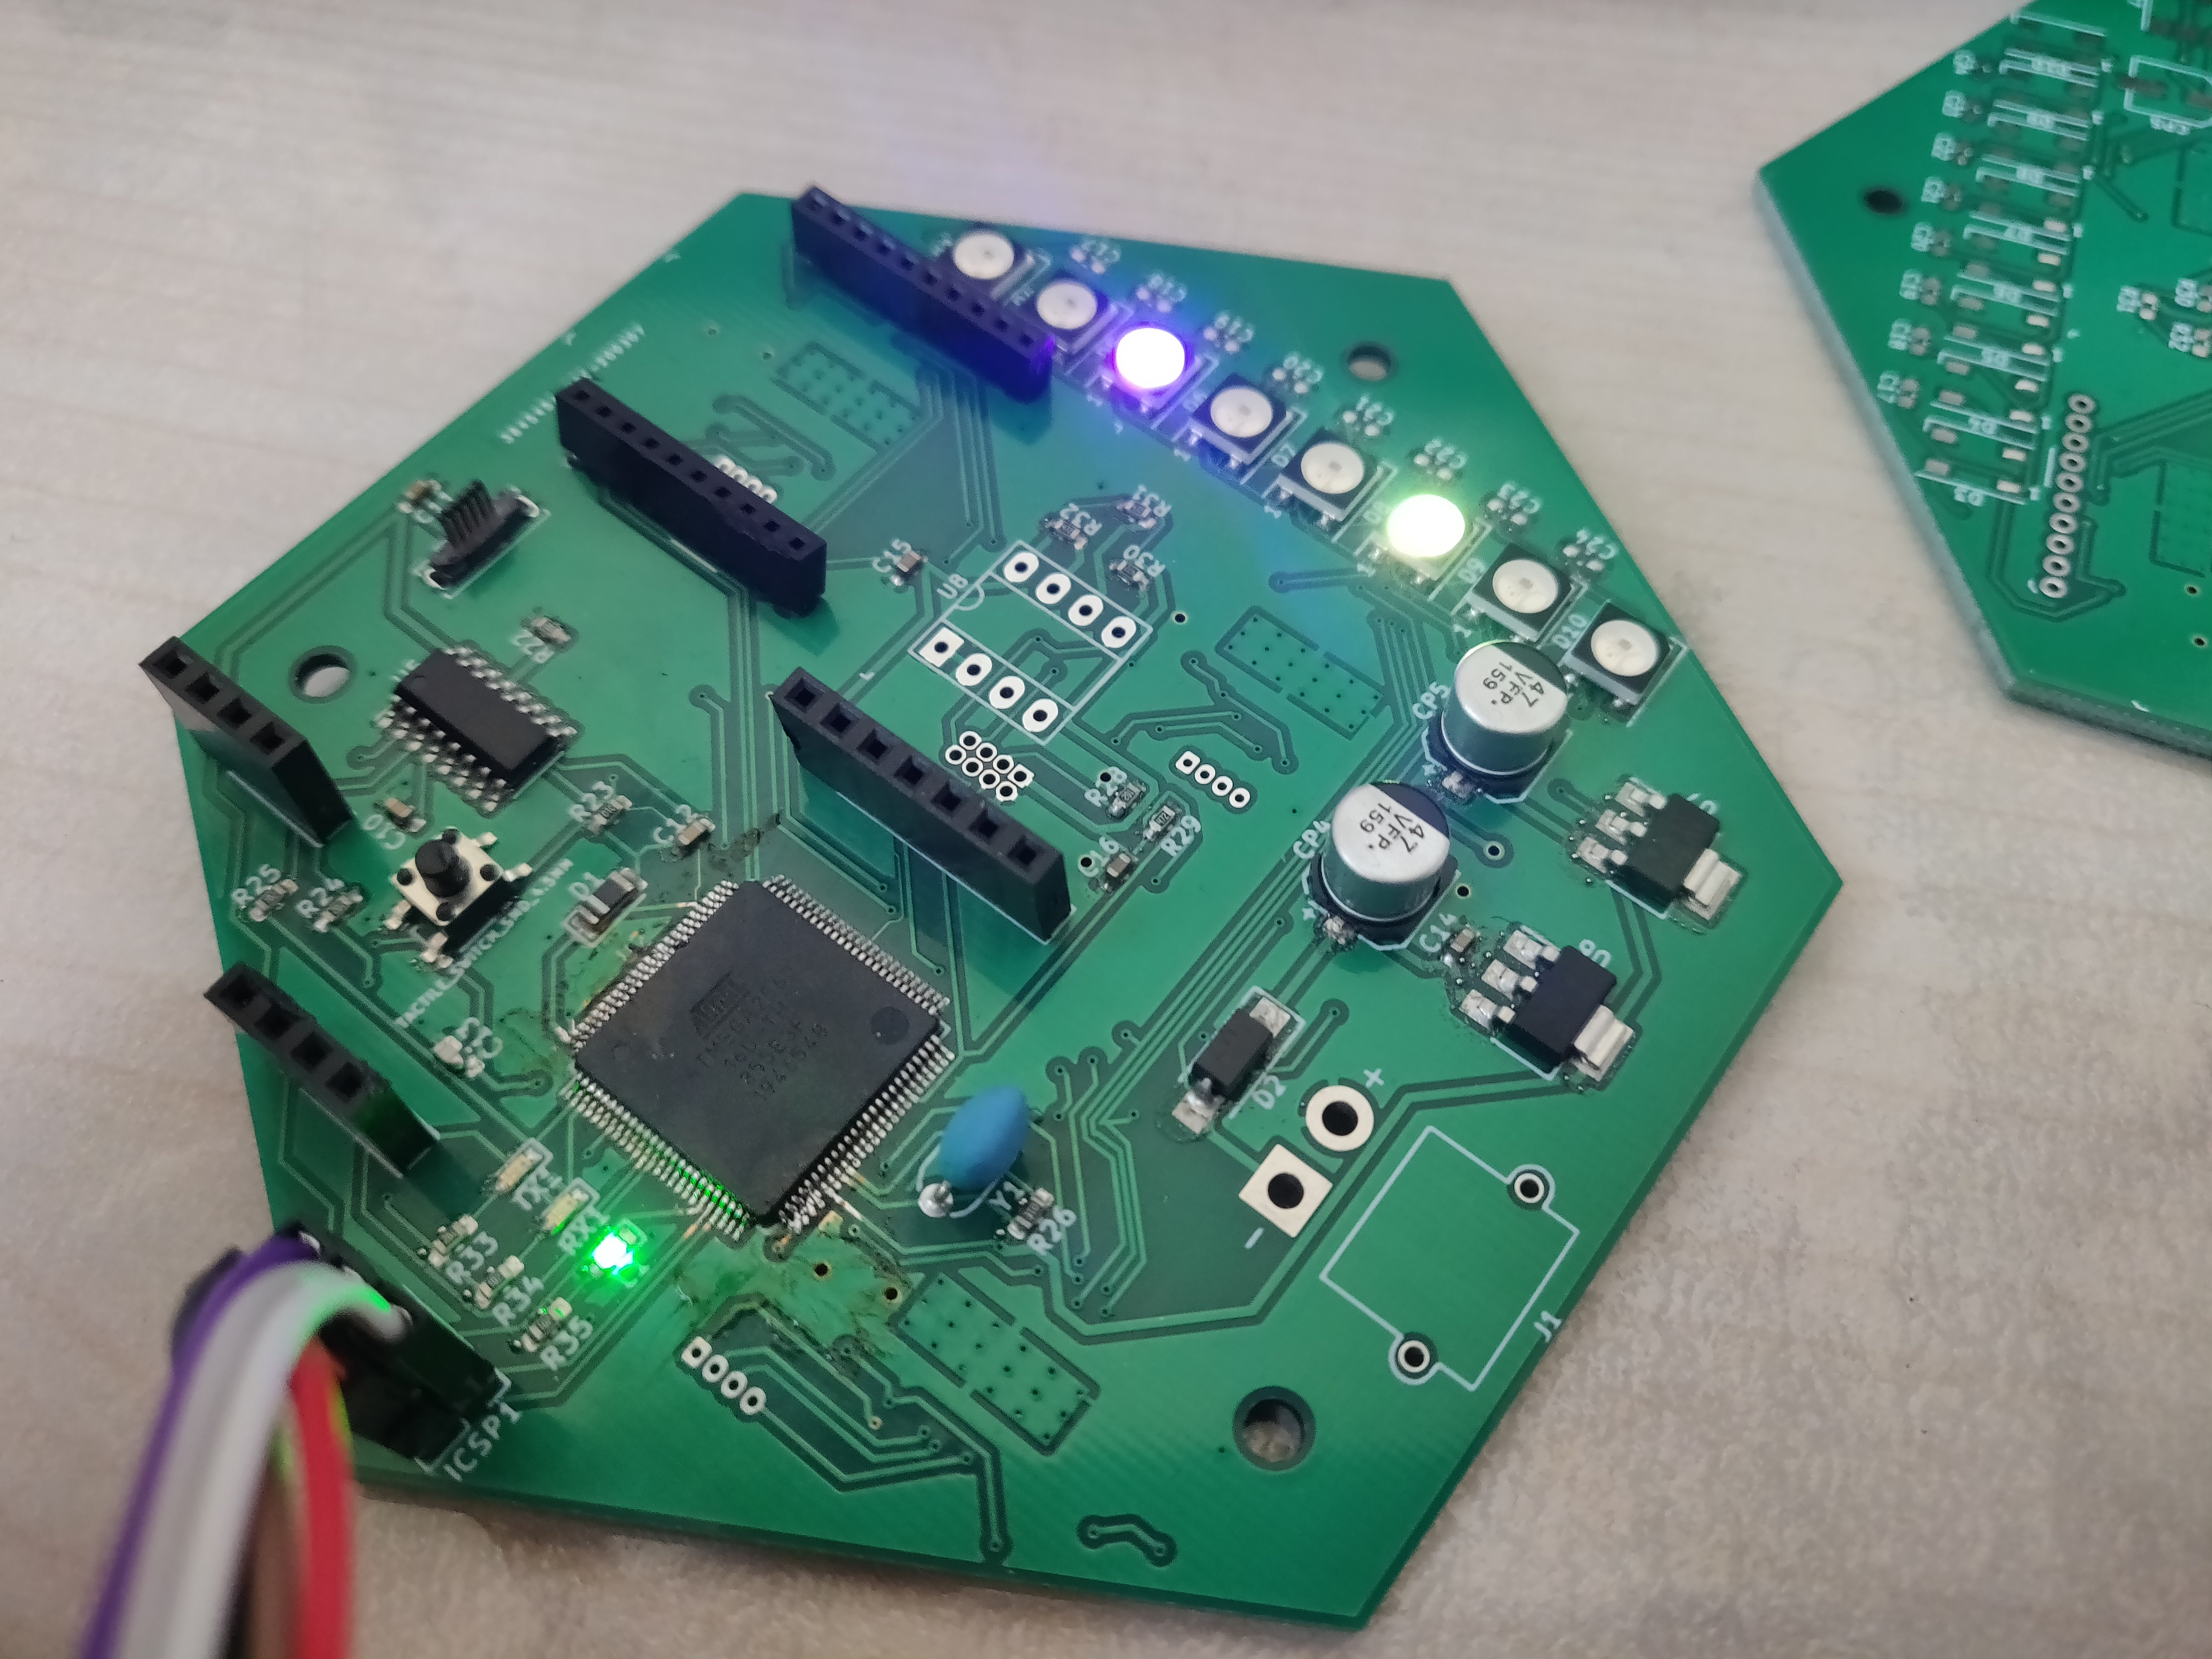
\includegraphics[width=\columnwidth]{PCBv2Test.jpg}
    \caption{Floar LED String Test程序运行效果}
    \label{fig:PCBv2Test}
\end{figure}

\section{Debug}

第一次通过USB上电就出现一个严重的问题,C12炸飞,火星四溅。烧毁的PCB如图~\ref{fig:BrokenPCB}。经过排查,是5V net经过C12下方的走线宽度过小,导致大功率经过时发热过大,把整条线路熔断,看到的火花并非电容爆炸时产生的,而是基板中的顶层铜层发热积累,破坏基板和阻焊之后过热的铜片产生的火花。如图~\ref{fig:BrokenPCB},当仅使用5V供电时,几乎所有元件的功率都叠加在C12下面的走线上,当初画的板子时不合理的。测试阶段暂时外接一个5V作为替代,等待新板子交货。

\begin{figure}[htbp]
    \centering
    \includegraphics[width=\columnwidth]{PCBv2BrokenPCB.jpg}
    \caption{烧毁的PCB}
    \label{fig:BrokenPCB}
\end{figure}

\begin{figure}[htbp]
    \centering
    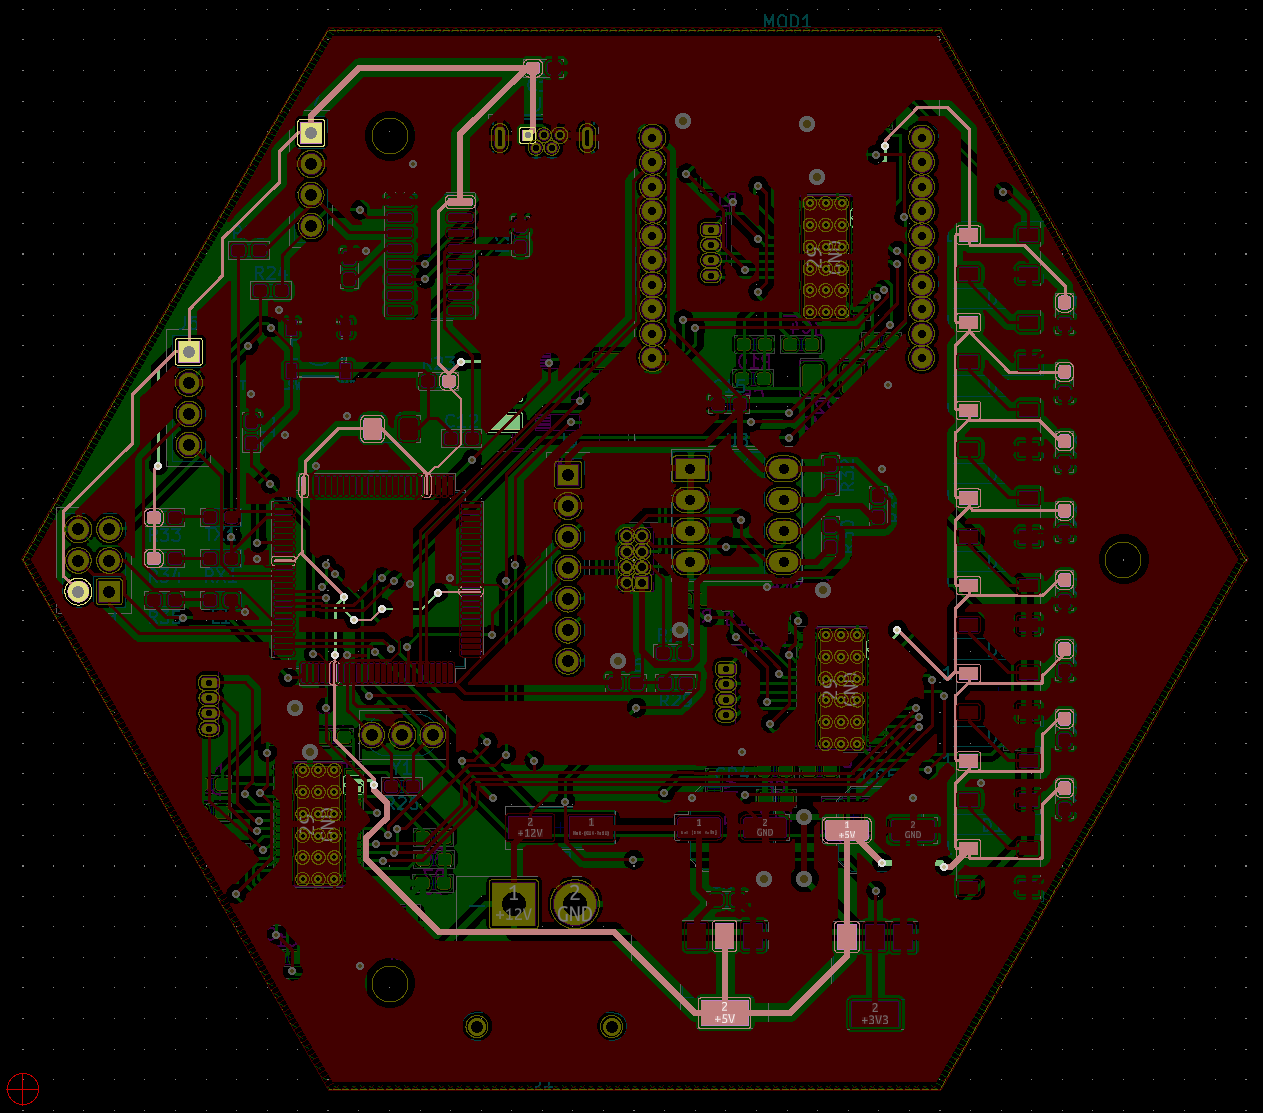
\includegraphics[width=\columnwidth]{BrokenPCB-5V.png}
    \caption{5V net 存在的串联瓶颈问题}
    \label{fig:BrokenPCB-Illumination}
\end{figure}

以及焊接的时候,用除去多余焊锡的烙铁头解决AT Mega引脚相连问题时,400度加热时间过长,导致芯片损坏,使用ISP烧写程序时时断时续。

重新画了PCB,4月3日终于打样完成。

4月5日焊接完成了新板子的电机驱动系统,但是上午测试了一组,电机一直没有转,没找到原因,由于一共三组电机的驱动,下午把三组驱动都焊完了,发现只有三号电机驱动是能用的,电机在转,其他两个都没转,不知道为什么,好在有能用的说明原理上没有问题,有可能是我焊的时候哪里出错了,得仔细找找。

首先排查输入,D6输出的方波脉冲如图~\ref{fig:DRV8825Debug1}。

\begin{figure}[htbp]
    \centering
    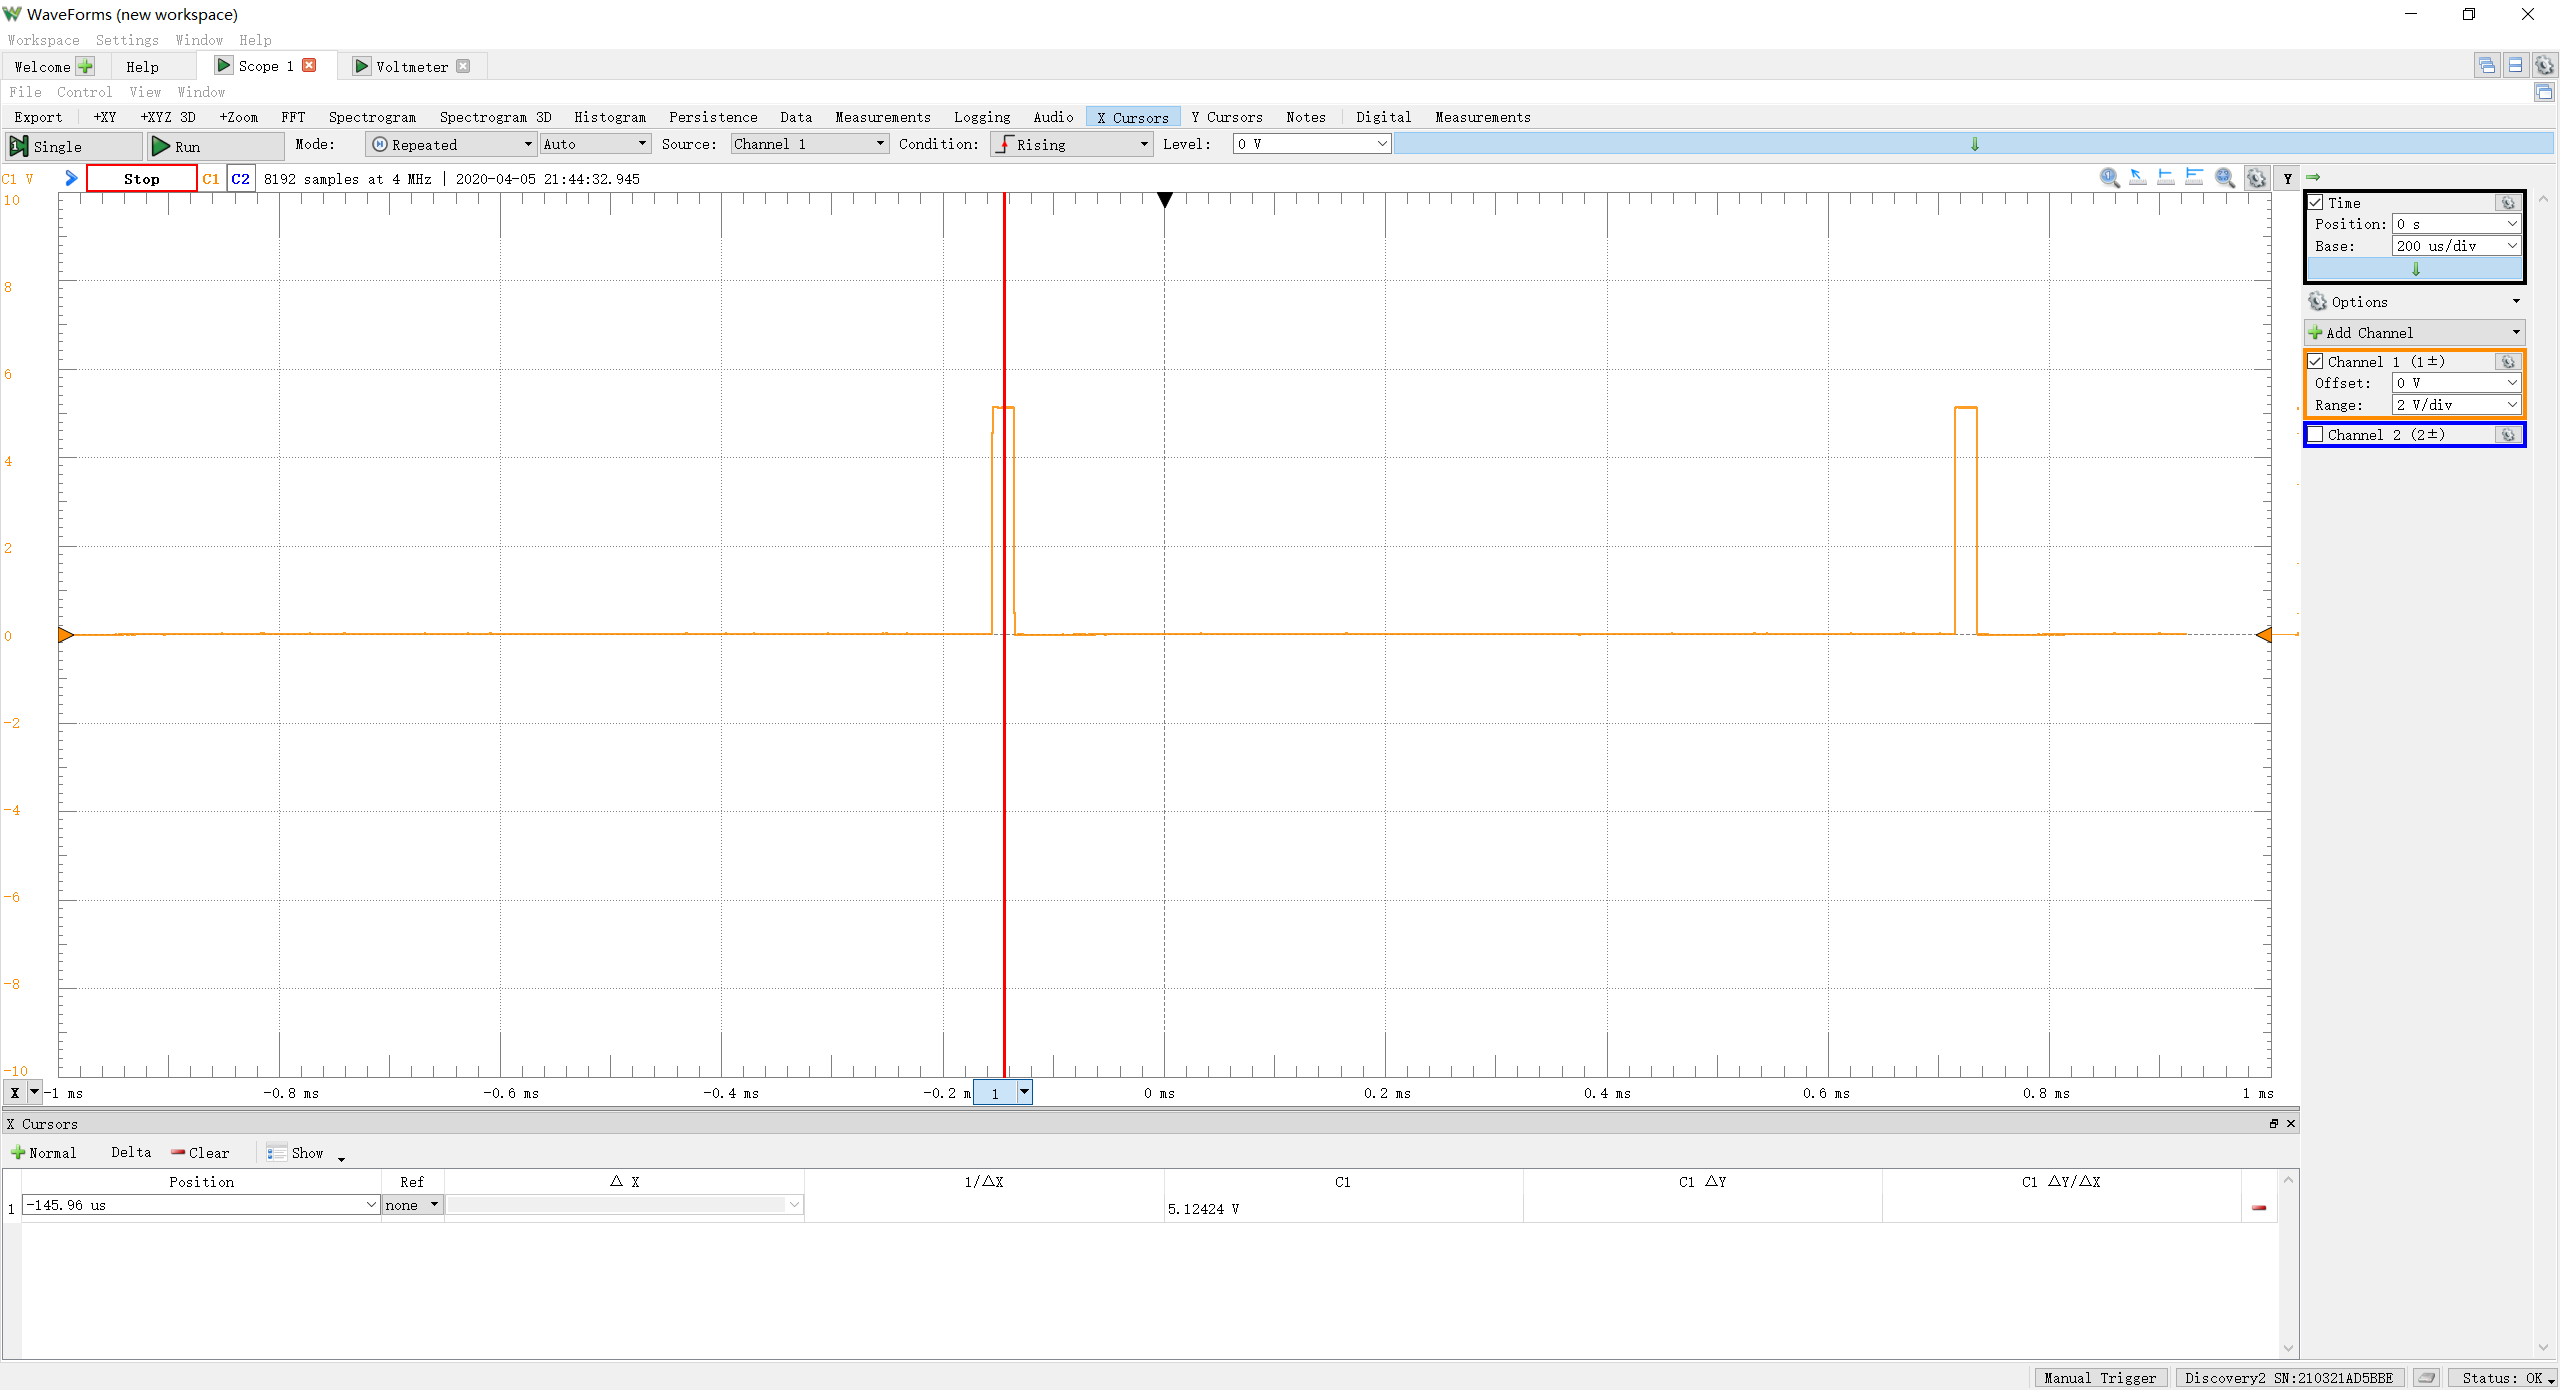
\includegraphics[width=\columnwidth]{DRV8825Debug1.png}
    \caption{D6输出的方波脉冲}
    \label{fig:DRV8825Debug1}
\end{figure}

用AD2排查发现借上12V电源后,发现3号DRV8825的12/13脚(AVREF/BVREF)电压为3.3V,但是1号为1.23V,2号为0.01V,可能IFS(Target Full-Scale Current)不足以驱动此步进电机。但实际上输出端根本没有方波信号输出,所以可能另有原因。而且3号电机发热严重,3.3V对应的IFS可能不合适。

按照我的设计1.23V是正常的,非常意外出现了3.3V和0V,现在拆掉R3和R9,让1号和2号的DRV8825的12/13脚(AVREF/BVREF)电压为3.3V。

2号空载时输出了PWM波,但是带不动电机,仔细排查发现13旁边的14号引脚(GND)和13连起来了,使得VREF一直处于低电平。使用蘸松香的350度刀头烙铁轻触连接的小块焊锡后正常。

\begin{figure}[htbp]
    \centering
    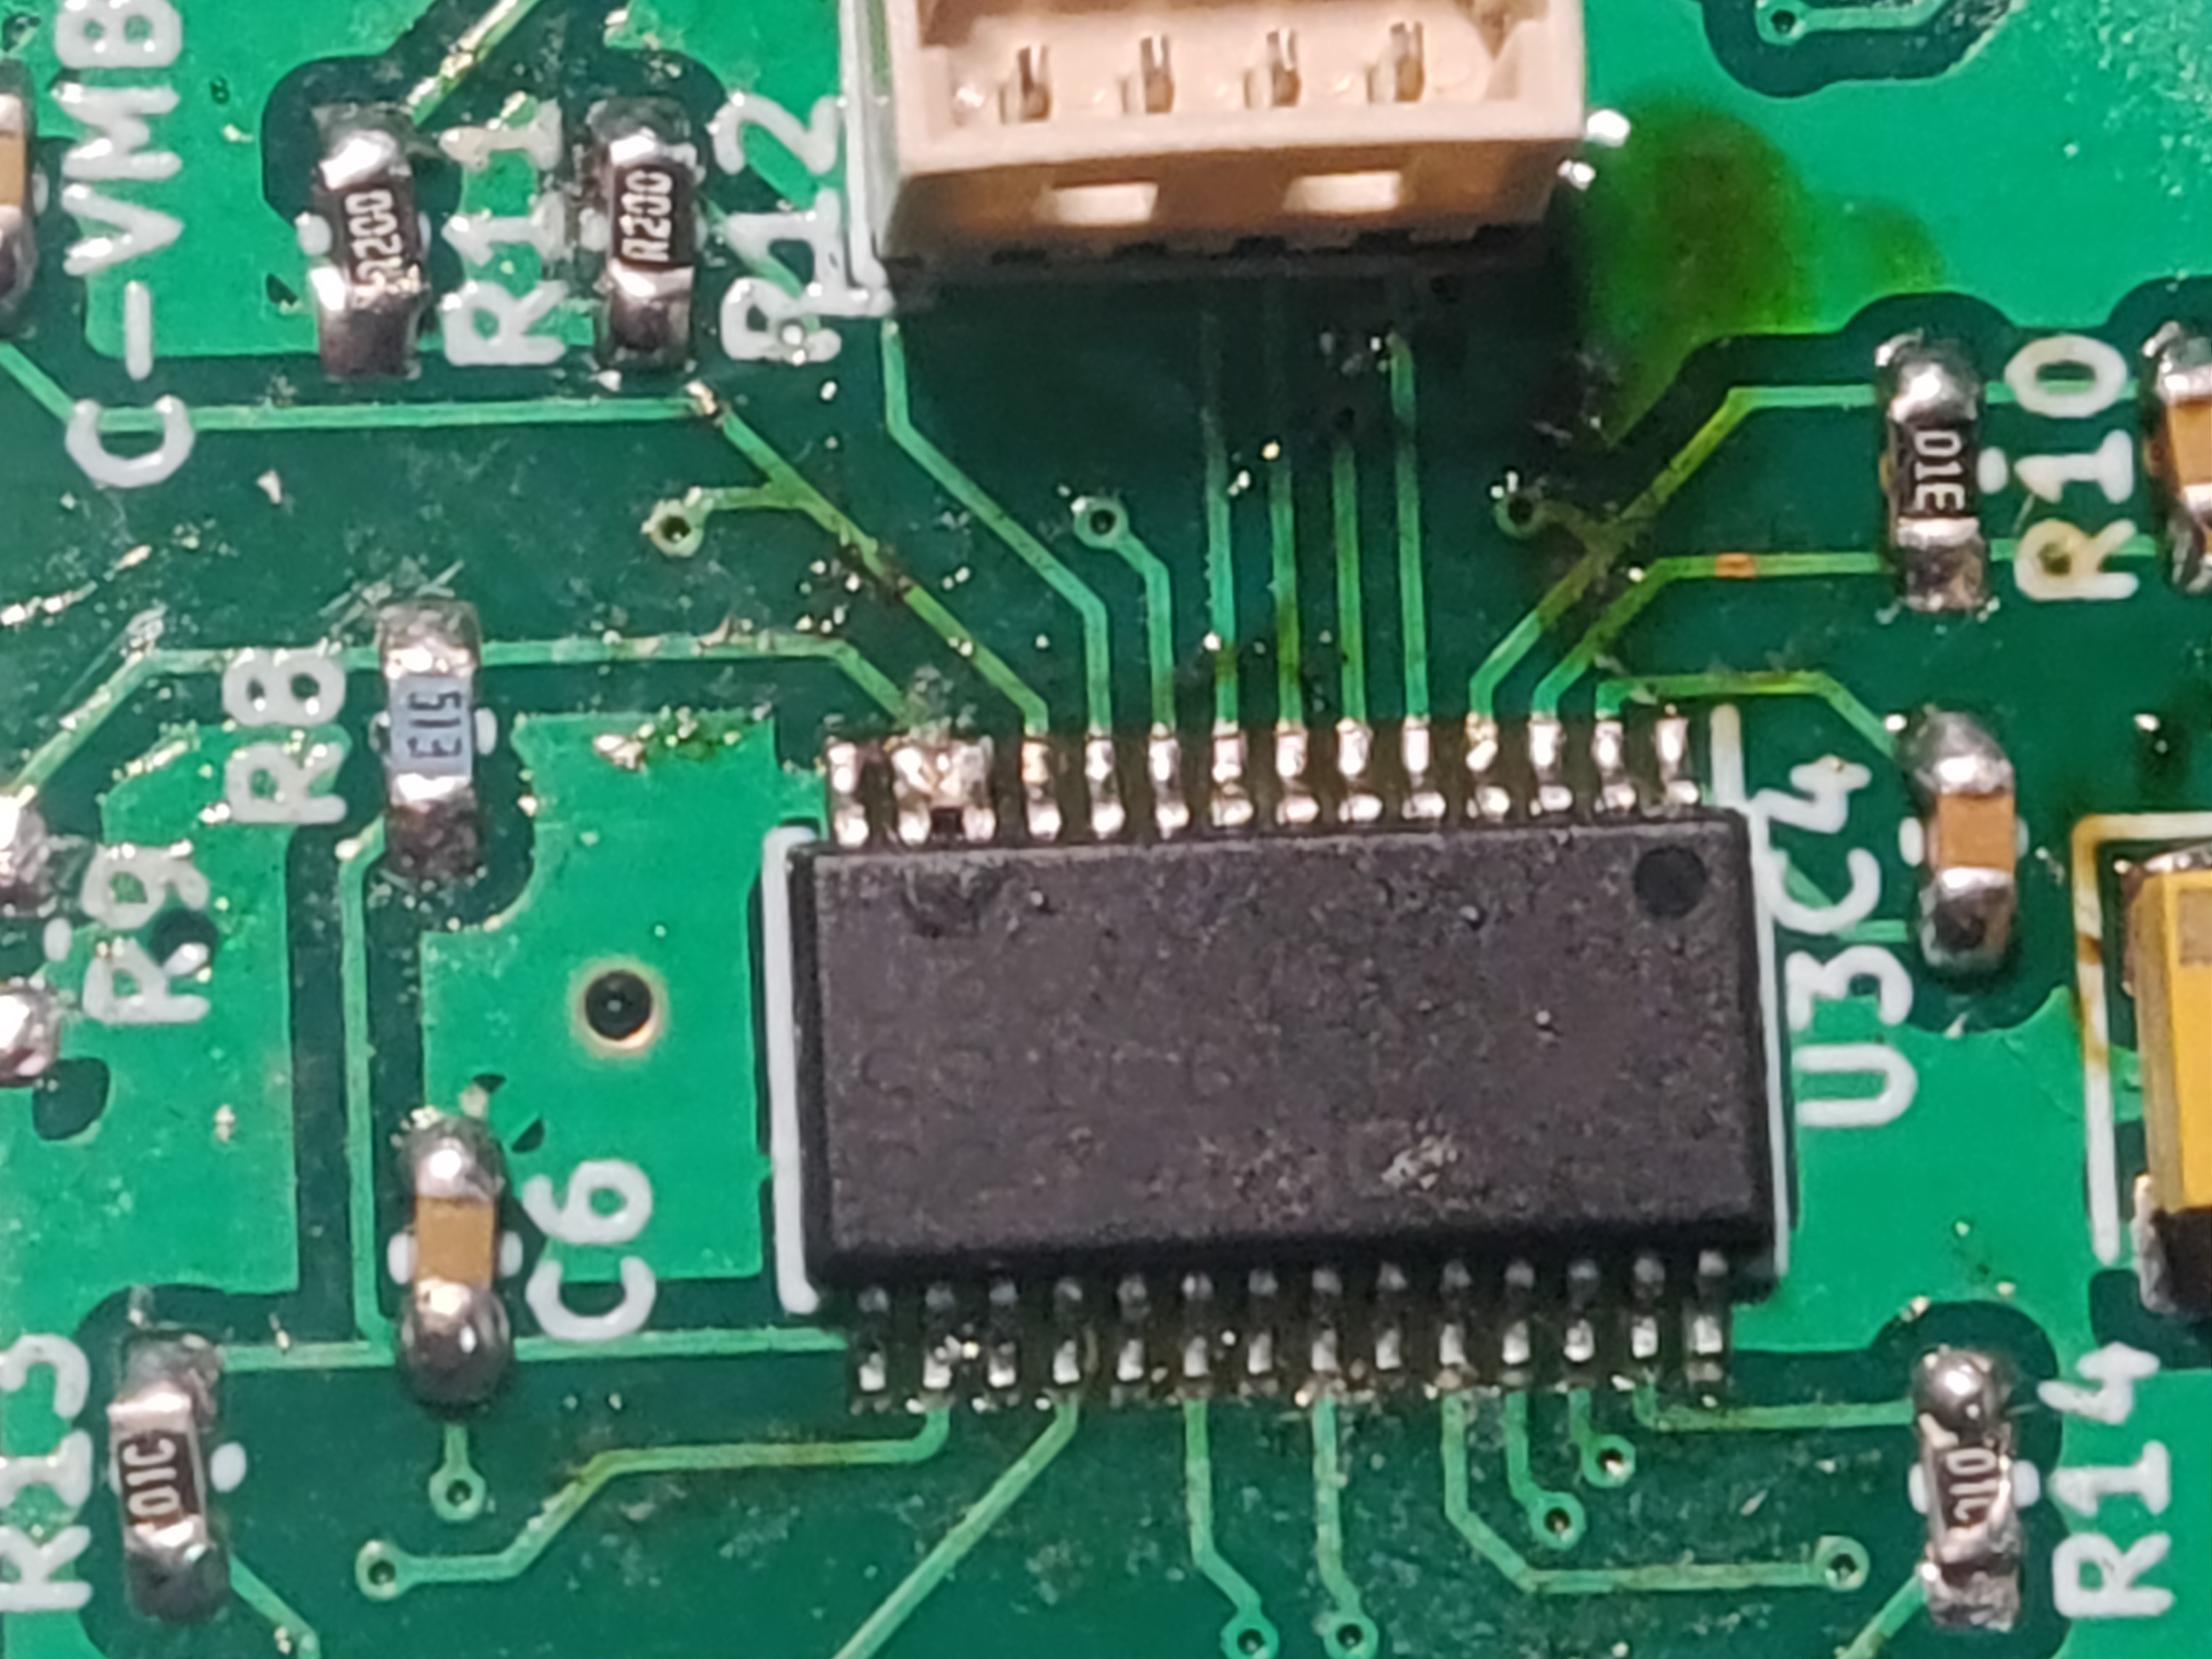
\includegraphics[width=0.8\columnwidth]{DRV8825Debug2.jpg}
    \caption{左上角的第1个和第2个角连起来了}
    \label{fig:DRV8825Debug2}
\end{figure}

1号空载时就没有输出PWM波,经排查,其27脚(nHOME)没有输出类似2/3号输出的方波,如图~\ref{fig:DRV8825Debug-25},查阅Datasheet得知,Home position : Logic low when at home state of step table,;类型为OD = open-drain output。R7为OD门的上拉电阻。

\begin{figure}[htbp]
    \centering
    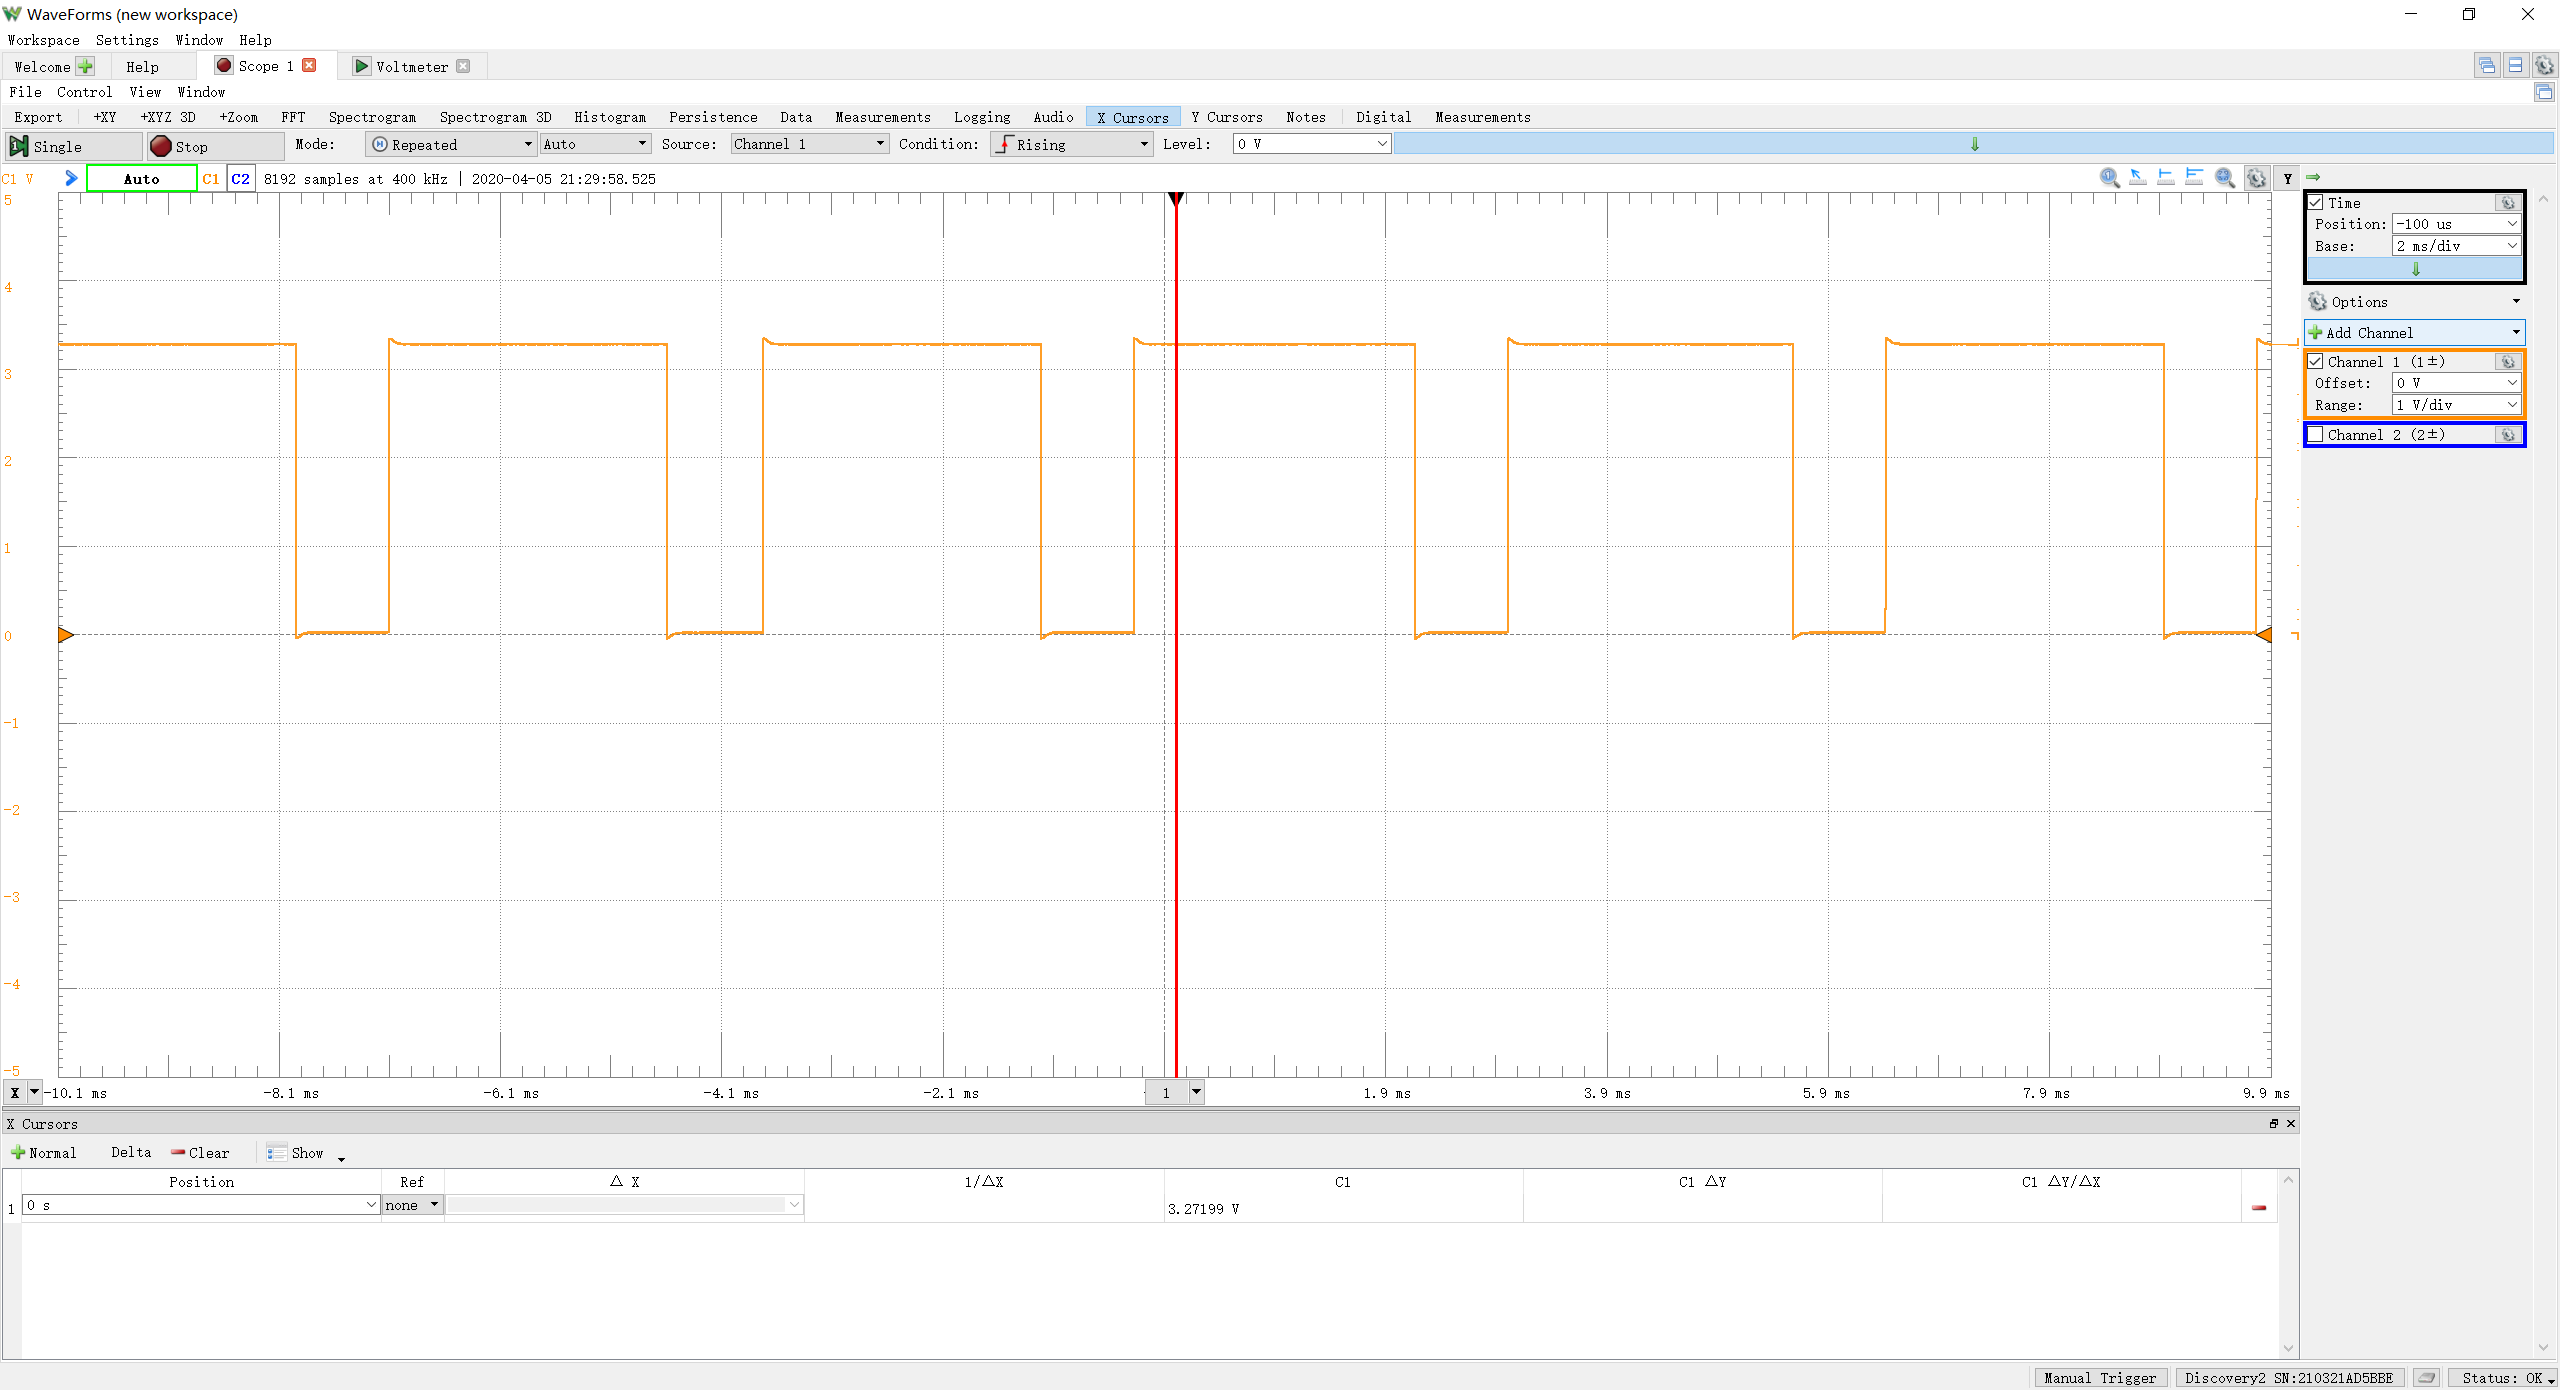
\includegraphics[width=\columnwidth]{DRV8825Debug3.png}
    \caption{2/3号27脚(nHOME)输出的方波}
    \label{fig:DRV8825Debug-25}
\end{figure}

排查了所有输入引脚和滤波电容,没有发现问题,应该时芯片损坏了。